%
% A simple LaTeX template for Books
%  (c) Aleksander Morgado <aleksander@es.gnu.org>
%  Released into public domain
%
\RequirePackage{lineno}
\linenumbers 
\documentclass{article}
\usepackage[a4paper, top=3cm, bottom=3cm]{geometry}
%\usepackage[latin1]{inputenc}
%\usepackage{setspace}
\usepackage{fancyhdr}
%\usepackage{tocloft}
\usepackage{verbatim}
\usepackage{graphicx,amsmath,epsfig,color,amsfonts,relsize,subfigure}
\usepackage{authblk}
\usepackage{caption}
%\usepackage{subcaption}
%\usepackage[running]{lineno}
\begin{document}

 
%\pagestyle{empty}
%\begin{flushleft}
\pagenumbering{}
% Set book title
\title{\textbf{Thesis}}

\author{Ekaterina Avdeeva}

\affil{University of Nebraska-Lincoln, USA}
\maketitle
%\end{flushleft}

\begin{abstract}
This paper reviews
\end{abstract}

% 2nd page, thanks message
%-------------------------------------------------------------------------------
%\thispagestyle{empty}
%\newpage


% General definitions for all Chapters
%-------------------------------------------------------------------------------

% Define Page style for all chapters
\pagestyle{fancy}
% Delete the current section for header and footer
\fancyhf{}
% Set custom header
\lhead[]{\thepage}
\rhead[\thepage]{}

% Set arabic (1,2,3...) page numbering
\pagenumbering{arabic}
\tableofcontents
\linespread{1.5}

%
% Not enumerated chapter
%-------------------------------------------------------------------------------
%\linenumbers


\chapter{Introduction}
\label{sec:intro}

Elementary particle physics describes fundamental particles and their interactions. Fundamental particles are the smallest constituents of our Universe. When examined at smaller scales, the substances around us consist of molecules, molecules consist of atoms. In an atom there is a nucleus made of neutrons and protons and some number of electrons occupying orbits around the nucleus. Protons and neutrons have a structure while an electron is not known to have any internal structure, therefore, an electron is an example of a particle which is considered to be fundamental.

Interactions of elementary particles are described by quantum field theories which incorporate principles of the quantum mechanics and the special theory of relativity. The set of such theories, including quantum elecrtrodynamics (QED), quantum chromodynamics (QCD) and the theory of weak interactions is called the Standard Model (SM). Current observations have proved the SM to be an accurate description of elementary particle interactions.  

However, there are several experimental observations that are not described by the SM such as effects of gravity, dark matter, dark energy, matter/antimatter asymmetry and others. Therefore, the SM is not a complete theory of particle interactions. There are several SM extensions offered by theorists as well as radically new theories waiting for experimental confirmation or exclusion. 

Some SM extensions and new theories predict the existence of heavy particles with masses lying beyond experimentally reachable energies. The search of these particles is a priority in particle physics. One source of highly energetic elementary particles is cosmic rays. The most energetic particles ever observed came from this source. However, cosmic rays are totally uncontrollable and such highly energetic particles are rare. If we want to produce a large number of particles in a given energy range, we need to use a particle accelerator. A large amount of data allows experimentalists to perform a statistical analysis and increase the probability of finding a new particle if it exists.

Symmetric colliding beams is the most effective way to produce as heavy particles as possible given the energies of the colliding particles. Compared to experiments colliding a single beam at a fixed target, in the case of a symmetric collision the total momentum of two colliding particles is zero and, therefore, much larger fraction of energy can transfer to a mass of a new particle.  The Large Hadron Collider (LHC) is one such collider with the highest energy in the world. It can produce the most massive particles to probe physics beyond the SM (BSM). 
%It collides two proton ($pp$) beams, two lead ion beams ($Pb-Pb$) or a proton beam to a lead ion beam ($p-Pb$). The design energies for a colliding proton and a colliding lead ion at LHC are~7~TeV and~522~TeV respectively. \\

The Compact Muon Solenoid (CMS) is one of two general-purpose detectors at the LHC. It is placed at one of four collision points. CMS has a broad physics program including searches for the BSM physics as well as the precision measurements of the parameters of the SM itself. The measurement of this dissertation is a SM measurement with CMS data collected in~2012 in $pp$ collisions of LHC with beam energies of~4~TeV. The result can be compared to the SM prediction. Certain BSM theories predict a deviation of the result of this measurement from its SM value, therefore, with this measurement, in addition to testing the SM, we also search for a new physics.

%In this dissertation, the study of $pp\rightarrow W\gamma + X$ process where the $W$ decays as $W\to \ell\nu$ where $\ell = e, \mu$ is reported. The $W\gamma$ production with leptonic $W$ decays proceeds through one of the following three processes: the initial state radiation where a photon is emitted from one of the incoming partons, the final state radiation where a photon is radiated off the charged lepton from the $W$ boson decay, and, finally, the triple gauge coupling (TGC) where a photon is emitted from the $W$ boson. Many BSM theories predict an enchancement of the TGC production over the SM value and, therefore, the experimental search for such an enchancement is a good test for such theories.\\ 
%The total and the differential cross section with respect to the photon transverse momentum ($P_T^\gamma$) has been measured. The $P_T^{\gamma}$ is sensitive to the potential anomalous TGC (aTGC) in the high $P_T^{\gamma}$ region. The disagreement between the measured and theoretically predicted differential cross section at the higher $P_T^{\gamma}$ end would be an indication of the possible presence of the aTGC. \\

The rest of this chapter gives general introductory information about the SM while Ch.~\ref{sec:WgAbout} concentrates on the theory of the SM and BSM $W\gamma$ production and also discusses previous measurements of this process. Chapter~\ref{sec:Exp} describes LHC and CMS in more details. Chapter~\ref{sec:alignment} explains one specific detail of the CMS operation that is the spacial alignment of the tracking detector of charged particles. Finally, Ch.~\ref{sec:AN_WgMeas} describes the details of the measurement of this dissertation and reports the results. 

%\subsection{Fundamental Particles and Interactions}
\label{sec:Intro_FundParticles}

The SM describes interactions of elementary particles. There are four fundamental interactions: electromagnetic, strong, weak and gravitational. The gravity is not included into the SM but its effect on particles is negligible compared to the other forces which makes it possible to develop a theory of the particle physics and conduct experiments even without having the gravity included into the model.\\ 

All fundamental elementary particles in the SM can be split into three categories by their spins. There are fermions which possess spin s=1/2, there are gauge bosons which are vector particles (s=1) and there is the Higgs boson which is a scalar particle (s=0). \\

The fermions are arranged into three generations, each generation consists of a quark with charge Q=$+$2/3(up, charm, and top quarks), a quark with Q=$-$1/3 (down, strange, and bottom quarks), a charged lepton with Q=$-$1 (electron, muon, and tau-lepton) and a neutrino (electron, muon, and tau neutrinos) which is electrically neutral. Each quark can carry any of three colors: red, blue, or green. Additionally, each fermion has its antiparticle. Therefore, the total number of fundamental fermions is $(6 ($leptons$)+6 ($quarks$) \cdot 3 ($colors$) ) \cdot 2 ($to~include~antiparticles$) = 48$.\\ 

Corresponding particles in different generations have the same charges, spins and interaction properties but masses of particles increase with a generation. These mass differences lead to different decay properties because a particle A can decay to particles B and C only if the mass of A $m_A > m_B + m_C$. Thus, an electron is a stable particle, a muon decays as $\mu^- \rightarrow e^- + \bar{\nu_e} + \nu_\mu$, a tau-lepton, as the heaviest charged lepton, has the largest number of decay channels amongst the charged leptons: $\tau^- \rightarrow \mu^- + \bar{\nu_\mu} + \nu_\tau$, $\tau^- \rightarrow e^- + \bar{\nu_e} + \nu_\tau$,  $\tau^- \rightarrow \nu_\tau +$ quarks. \\

In addition to fermions, the SM includes gauge bosons which are interaction mediators. They are called mediators because fermions interact with each other by exchanging them. For example, two charged fermions can interact with each other by exchanging a photon. Such interaction is called electromagnetic interaction and a photon is a mediator for the electromagnetic interaction. Similarly, a gluon is a mediator for the strong interactions, and W$^{\pm}$ and Z$^0$ bosons are mediators for the weak interactions. W$^{\pm}$ and Z$^0$ bosons are massive while a photon and a gluon are massless particles. \\

The last SM particle is the Higgs boson. The Higgs boson is a scalar neutral particle which is playing a critical role in the electroweak symmetry breaking. The Higgs mechanism describes how $W$ and $Z$ bosons become massive particles.\\

All the particles are summarized in Fig. \ref{fig:SMtable}. These and only these fundamental particles and their antiparticles have been discovered by now. However, there are many composite particles which are called hadrons. Hadrons can consist of three quarks (baryons), quark and antiquark (meson), or three antiquarks (antibaryons). Hadrons always possess an integer charge.\\

Most of the particles are short-lived and decay within microseconds. The only stable particles are protons and antiprotons, electrons and positrons, neutrinos and antineutrinos, photons, and, in some sense, gluons. However, if a particle cannot decay, it does not mean that it would live forever. There are many different kinds of reactions in which particles can disappear. Antiprotons and positrons would immediately annihilate with protons and electrons, photons can be absorbed by charged particles, electrons and protons can scatter to produce neutrons and neutrinos and many other reactions are possible.\\ 

In this dissertation a process is studied where quark and antiquark interact to produce a $W$ boson which then decay as $W^\pm \rightarrow e^\pm \nu_e(\bar{\nu_e})$ or $W^\pm \rightarrow \mu^\pm \nu_\mu(\bar{\nu_\mu}) $. A photon is radiated off a quark or antiquark, a charged lepton or a $W$ boson. The most interesting mechanism out of three is a radiation from a $W$ boson because this is the triple gauge coupling where we potentially can have a new physics. Therefore, the focus of this study is an interaction between a photon and a $W$ boson however many other SM particles are relevant too. Thus, a charged lepton and a neutrino appear as the final state particles, a quark and an antiquark appear as initial state particles and all fundamental particles except the Higgs boson participate in various background processes. Subsections \ref{sec:Intro_Electroweak}-\ref{sec:Intro_ppCollisions}, chapter \ref{sec:WgAbout} and \cite{ref_Griffiths} describe particle interactions in more details.\\


\begin{figure}[htb]
  \begin{center}
    {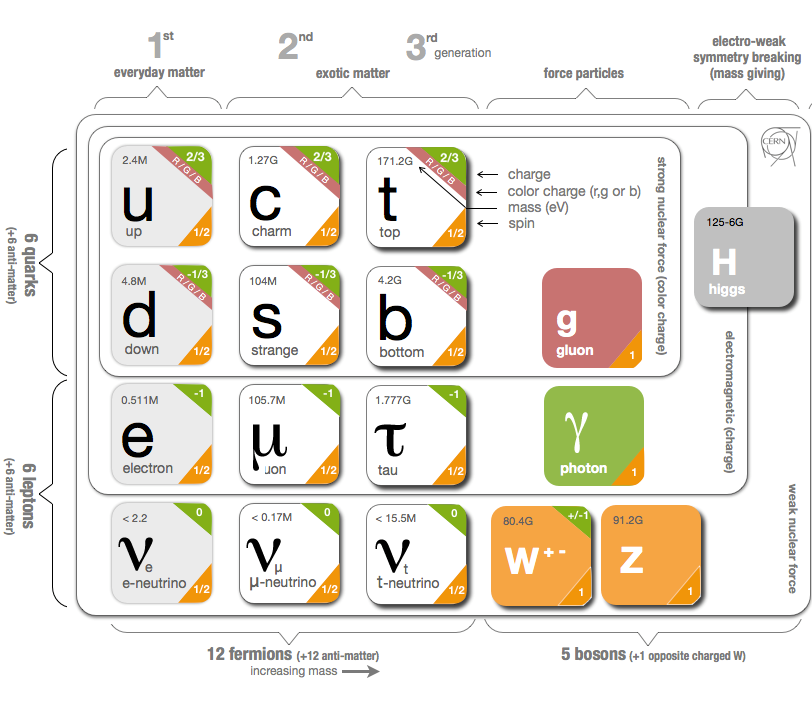
\includegraphics[width=0.90\textwidth]{../figs/Intro/StandardModel.png}}
    \caption{Standard Model Particles and Interations. Source of the figure: \cite{ref_fig_SM}.}
    \label{fig:SMtable}
  \end{center}
\end{figure}






%\subsection{Electroweak Interactions}
\label{sec:Intro_Electroweak}

\begin{figure}[htb]
  \begin{center}
    {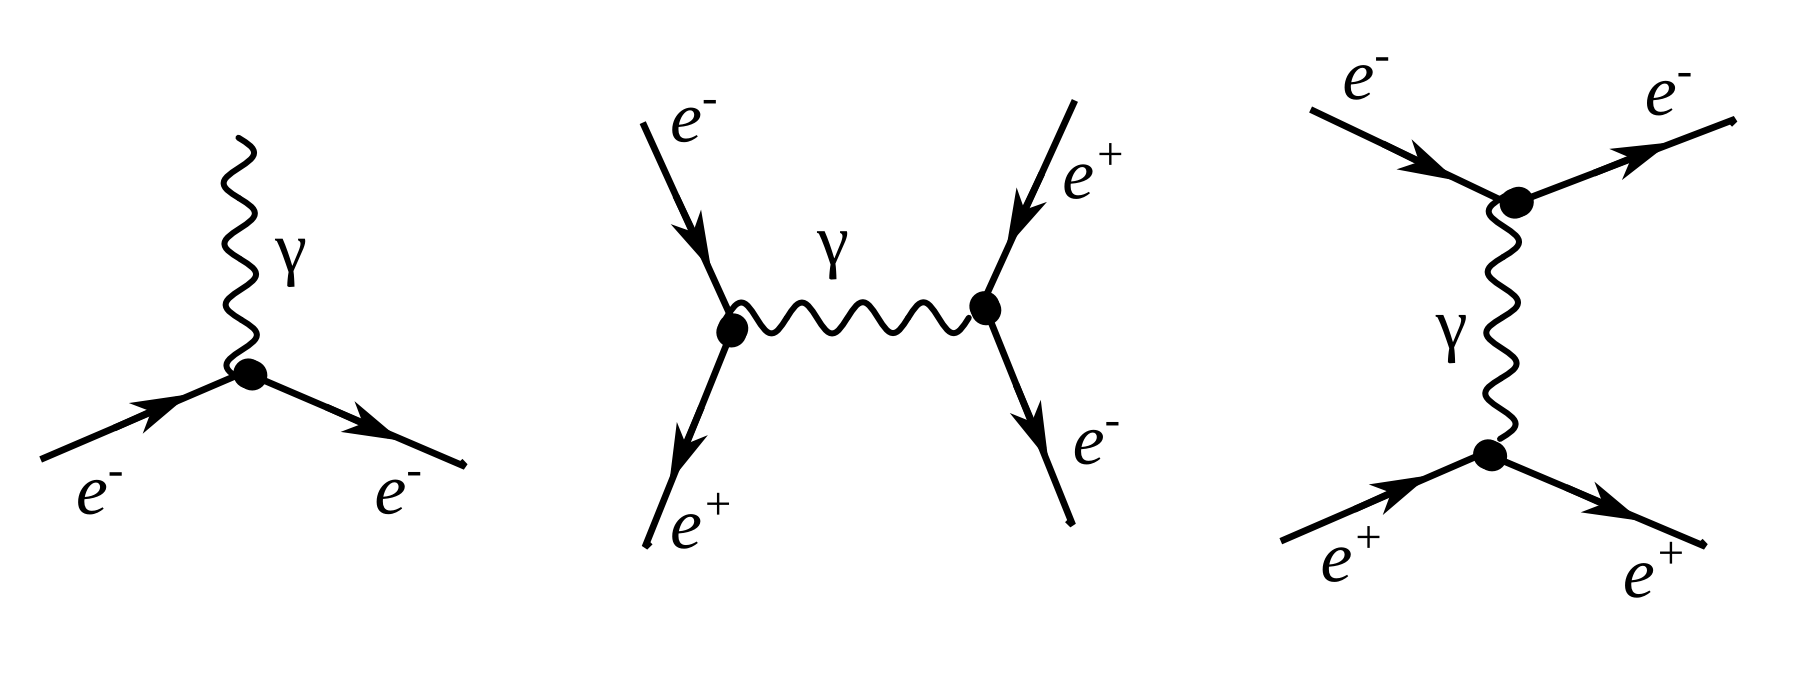
\includegraphics[width=0.90\textwidth]{../figs/Intro/feynmEM.png}}
    \caption{Electromagnetic interations}
    \label{fig:feynmEM}
  \end{center}
\end{figure}

\begin{figure}[htb]
  \begin{center}
    {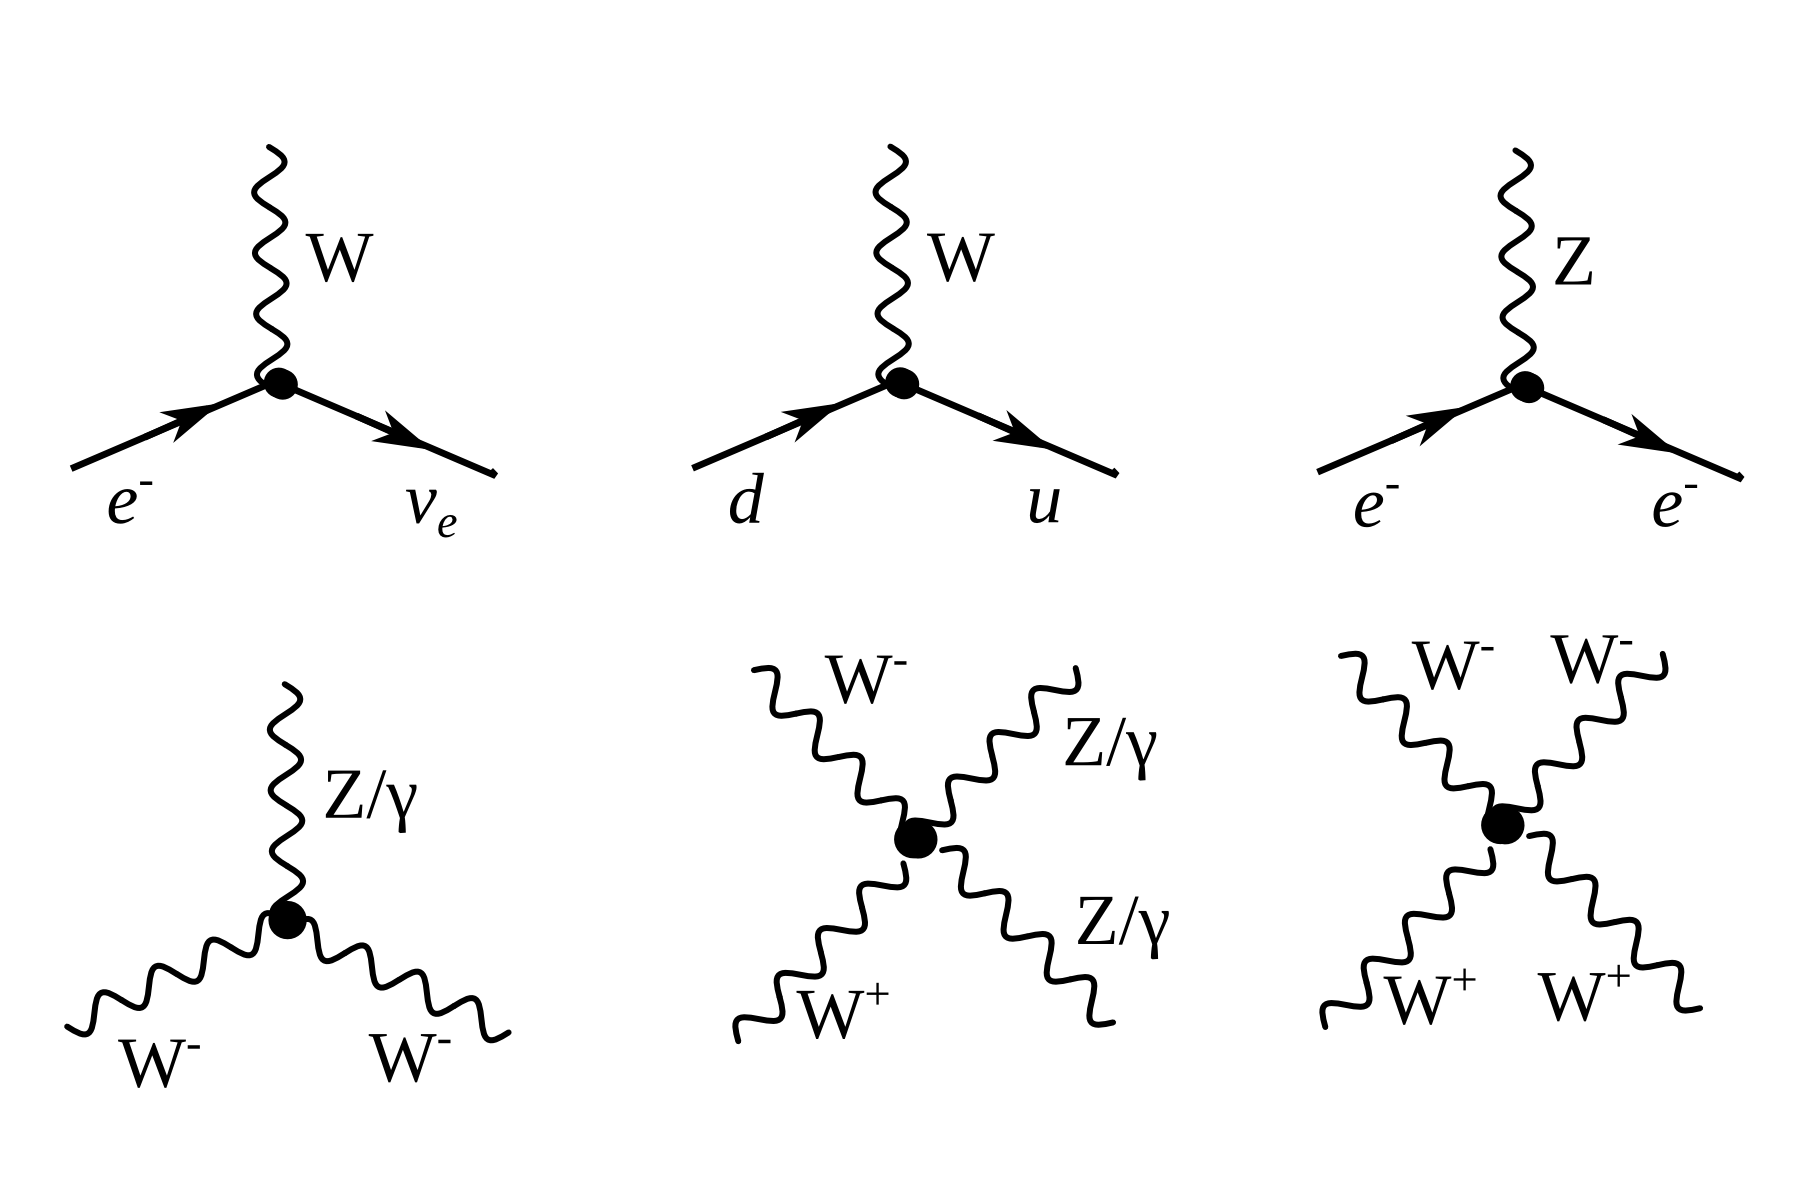
\includegraphics[width=0.90\textwidth]{../figs/Intro/feynmW.png}}
    \caption{Weak interations}
    \label{fig:feynmW}
  \end{center}
\end{figure}

All electrically charged particles participate in electromagnetic interactions. Photon, the mediator of the electromagnetic interactions, is a spin-one electrically neutral massless particle. All electromagnetic interactions can be reduced to one elementary process (Fig. \ref{fig:feynmEM}, left). This process reads: an electron enters, radiates or absorbs a photon, and escapes. Although there is an electron is drawn in this figure, it can be any other charged fermion as well. Such elementary process itself is forbidden by the energy conservation law but this element is a base of actual process (for example, Fig. \ref{fig:feynmEM}, middle and right). Such graphical representations of the particle physics processes are called Feynman diagrams. 

As for the weak interactions, there are two kinds of them: neutral (mediated by a Z boson) and charged (mediated by a W boson). Elementary processes with W and Z bosons are shown in Fig. \ref{fig:feynmW}. An electric charge must be conserved at any vertex. Therefore, if a charged lepton enters and radiates a W boson, a neutrino or antineutrino escapes (top left in Fig. \ref{fig:feynmW}). That is how a W boson interacts with a charged lepton and a neutrino. A lepton flavor number is always conserved in this interaction (Tab. \ref{tab:LeptonFlavorNumber}). 

 \begin{table}[h]
  \begin{center}
  \caption{ Lepton Flavor Number}
  \begin{tabular}{|c|c|c|c|}
     particles & $L_e$ & $L_{\mu}$ & $L_{\tau}$ \\ \hline
     $e^-,\nu_e$ &  +1  &  0  &  0  \\ \hline 
     $e^+, \bar{\nu_e}$ &  -1  &  0  &  0  \\ \hline 
     $\mu^-,\nu_{\mu}$ &  0  &  +1  &  0  \\ \hline 
     $\mu^+, \bar{\nu_{\mu}}$ &  0  &  -1  &  0  \\ \hline 
     $\tau^-,\nu_{\tau}$ &  0  &  0  &  +1  \\ \hline 
     $\tau^+, \bar{\nu_{\tau}}$ &  0  &  0  &  -1  \\ \hline 
  \end{tabular}
  \label{tab:LeptonFlavorNumber}
  \end{center}
\end{table}

From top middle diagram in Fig. \ref{fig:feynmW} we see that if a quark with Q=-1/3 enters, then a quark with Q=+2/3 escapes and, therefore, the flavor of the quarks has changed. The charged weak interaction is the only interaction which changes a quark flavor. The probability of each of three quarks with Q=+2/3 to be born is determined by the Cabibbo–Kobayashi–Maskawa matrix and is the highest for the quark of the same generation as an initial state quark (in this particular case, d is the initial state quark and u has the highest probability to be produced after an interaction with a W boson but c and t can also be produced if there is enough energy).

The right top diagram in Fig. \ref{fig:feynmW} is an emission of a Z boson off a fermion line. An electron is shown here as an example however it also could be any lepton, antilepton, quark or antiquark. All the same diagrams are possible with a photon instead of a Z boson except diagrams with neutrinos and antineutrinos.

The bottom diagrams in Fig. \ref{fig:feynmW} show self-coupling of a W boson, its interaction with Z boson and its electromagnetic radiation of a photon. WWZ, WW$\gamma$, WWZZ, WWZ$\gamma$, WW$\gamma\gamma$ and WWWW vertices are all possible in the SM.

Electromagnetic and weak interactions are unified by the electroweak theory. The mathematical formalism describing these two kinds of interactions is very similar. The difference between a photon and a Z boson is that a Z boson is massive and it can produce a neutrino-antineutrino pair or be scattered off a neutrino which a photon can not. The mass of Z boson is 91 GeV and that is why for low energies the probability of an electromagnetic process is much higher that the probability of similar neutral weak process. However, for particles with energies of E$\gg$91 GeV the mass of the Z boson can be neglected and these probabilities become the same. 

%\subsection{The Higgs Boson}
\label{Intro_Higgs}

% BAD SECTION
% NEEDS TO BE SIGNIFICANTLY REWORKED

\begin{figure}[htb]
  \begin{center}
    {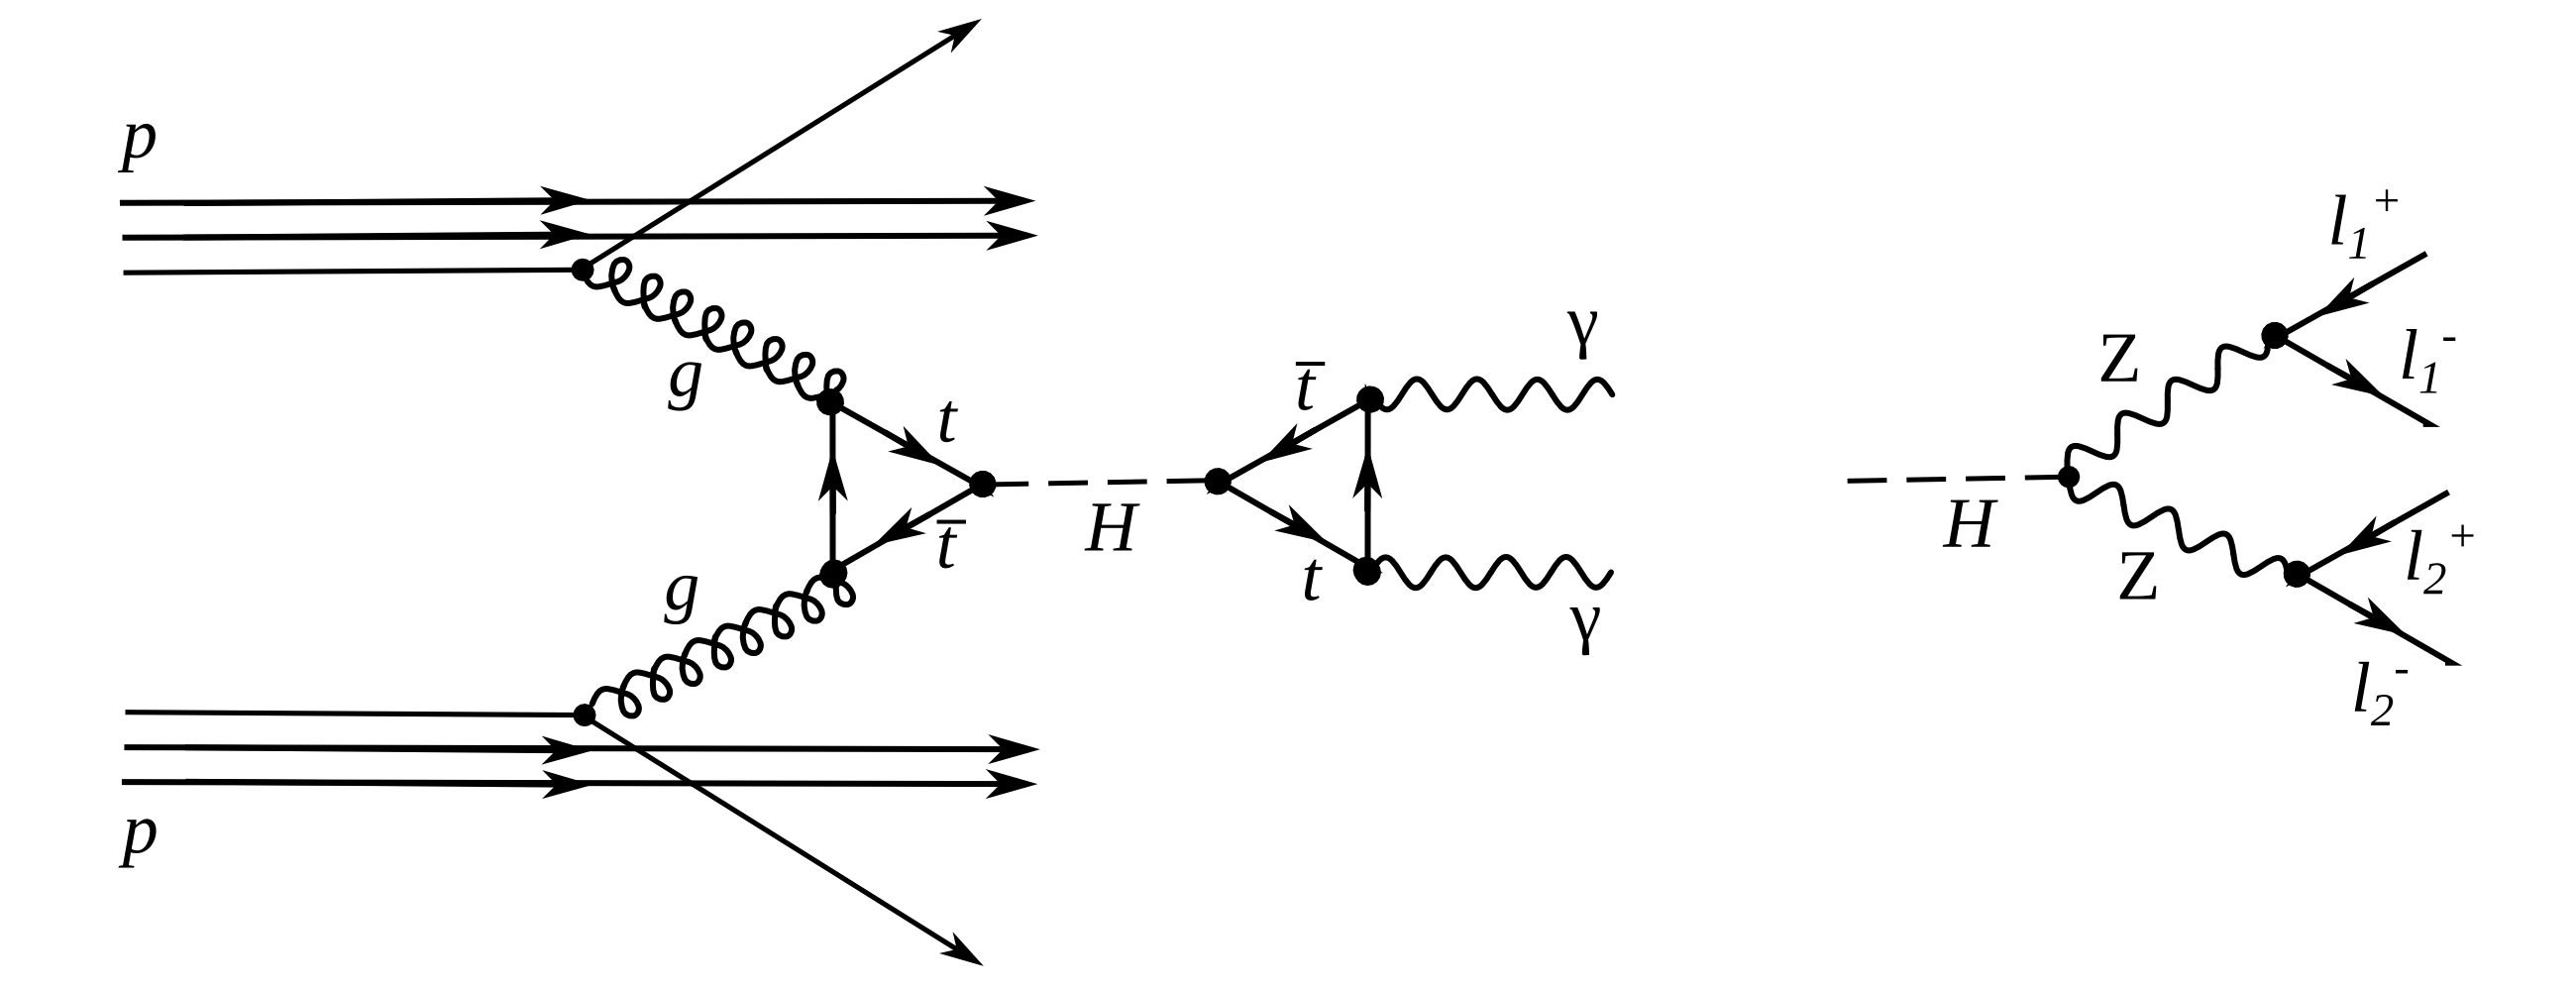
\includegraphics[width=0.95\textwidth]{../figs/Intro/FeynmanHiggs.png}}
    \caption{Higgs production and decay}
    \label{fig:higgsProduction}
  \end{center}
\end{figure}

%  I feel that there is a number of imprecise statements here that need to be corrected. Here are examples.
%   (A side note: quant is not what you mean, check the dictionary. You want to say “quantum”)
%   I would not say that the Higgs boson is a quantum of the Higgs field. The Higgs field is a doublet of complex fields, i.e. it has four components. According to wikipedia wording, for example, “it is a quantum excitation of one of the four components of the Higgs field. "
% This part: "discovered by ATLAS and CMS collaborations in the reaction shown in Fig. 4 in γγ and ZZ decay channels”
% The diagram in Fig. 4 is not appropriate for ZZ.
% "the same approach can be used to introduced masses of all elementary particles.” - but what about neutrinos? I am not sure if our favorite explanation of neutrino masses is the Higgs.
% It is not intuitive to me that larger mass means stronger interaction with the Higgs field,
% I am not sure why you say that.
% "that is how is gets its inertia”: consider rephrasing.









%\subsection{Strong Interactions}
\label{sec:Intro_QCD}

\begin{figure}[htb]
  \begin{center}
    {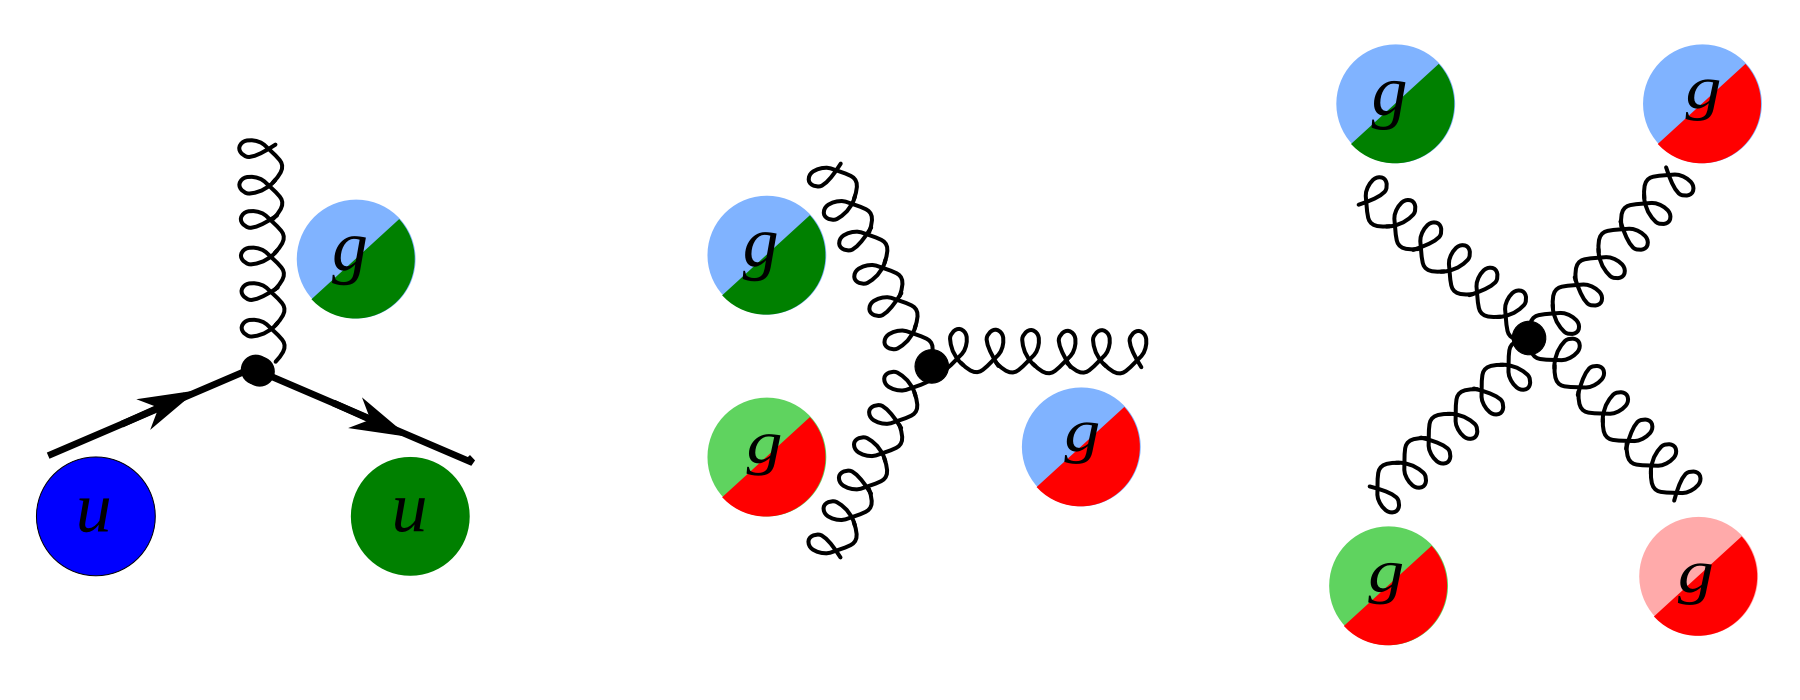
\includegraphics[width=0.80\textwidth]{../figs/Intro/feynmStrong.png}}
    \caption{Elementary processes of strong interations}
    \label{fig:feynmStrong}
  \end{center}
\end{figure}


The third fundamental force after the electromagnetic and weak ones is the strong force. The strong force is responsible for glueing protons and neutrons together in the nuclei as well as for forming protons and neutrons themselves. The strong interactions occur by exchanging gluons which are spin-one massless electrically neutral particles.  \\

The elementary strong processes are shown in Fig. \ref{fig:feynmStrong}. There are three elementary processes: $qqg$, $ggg$ and $gggg$, all are involving particles with color charges. Thus, gluons couple to quarks and self-couple. Color charges must be conserved at each elementary process of the strong interaction. Each quark possesses one of three colors at a time, and there are eight types of gluons to cover all possible color exchanges. \\

The coupling constant of the strong interaction depends on a distance between interacting particles: it becomes larger as the distance becomes larger and smaller as the distance becomes smaller. As the distance approaches zero, the coupling constant approaches zero too, and, thus, in the asymptotic limit two quarks located at the same place do not interact. This property is called asymptotic freedom.\\

On the other hand, when the distance between quarks becomes larger, the coupling constant also becomes larger. This property confines quarks to always stay in the color neutral combinations (hadrons), it forbids the existence of free quarks. A combination becomes color neutral when there is the same amount of color and anticolor or if there is the same amount of each of the three colors.  Thus, mesons are comprised of a quark and an antiquark with the opposite color charges, and baryons are comprised of three quarks: red, green and blue one. Examples of baryons include such well-known particles as a proton and a neutron.\\

The asymptotic freedom and the confinment are properties that are specific for strong interactions. The theory of strong interactions is called the QCD which is a quantum field theory invariant under $SU(3)$ color transformations. When the coupling constant is much less than one $\alpha_s \ll 1$, the perturbative approach can be used to compute observables.\\

The W$\gamma$ process being measured in this dissertation is not intended to test QCD, but a good understanding of QCD is essential for performing this measurement because the QCD corrections to the Feynman diagrams of the process are large and has to be taken into account in producing simulation. In addition, QCD describes the dynamics of quarks and gluons within colliding protons and predicts probabilities of one or another quark-antiquark pair to interact. Physics of proton-proton collisions is discussed in the subsection \ref{sec:Intro_ppCollisions}. \\

% Possible QCD corrections include quark-gluon loops at any of three quark lines as well as exchanges of gluons between different quark lines. 

%\section{Physics of Proton-Proton Collisions}
\label{sec:Intro_ppCollisions}

Consider a $pp$ collision at LHC. The proton energies are so high that each proton behaves as a complex structure. A proton is a baryon, it consists of three quarks: $uud$. These three quarks are called valence quarks. They interact with each other by exchanging gluons which produce virtual $q\bar{q}$ pairs (Fig.~\ref{fig:ppCollision}). Such virtual quarks are also called sea quarks. 

Any parton, quark, antiquark or gluon, from one proton can interact with any parton from another proton. Probabilities $f_i(x,Q^2)$ of any particular constituent $i$ to interact are described partially by QCD and partially by experimental measurements and depend on the momentum transfer $Q$ and the momentum fraction of a specific parton $x$. These probabilities are called parton distribution functions (PDFs).

\begin{figure}[htb]
  \begin{center}
    {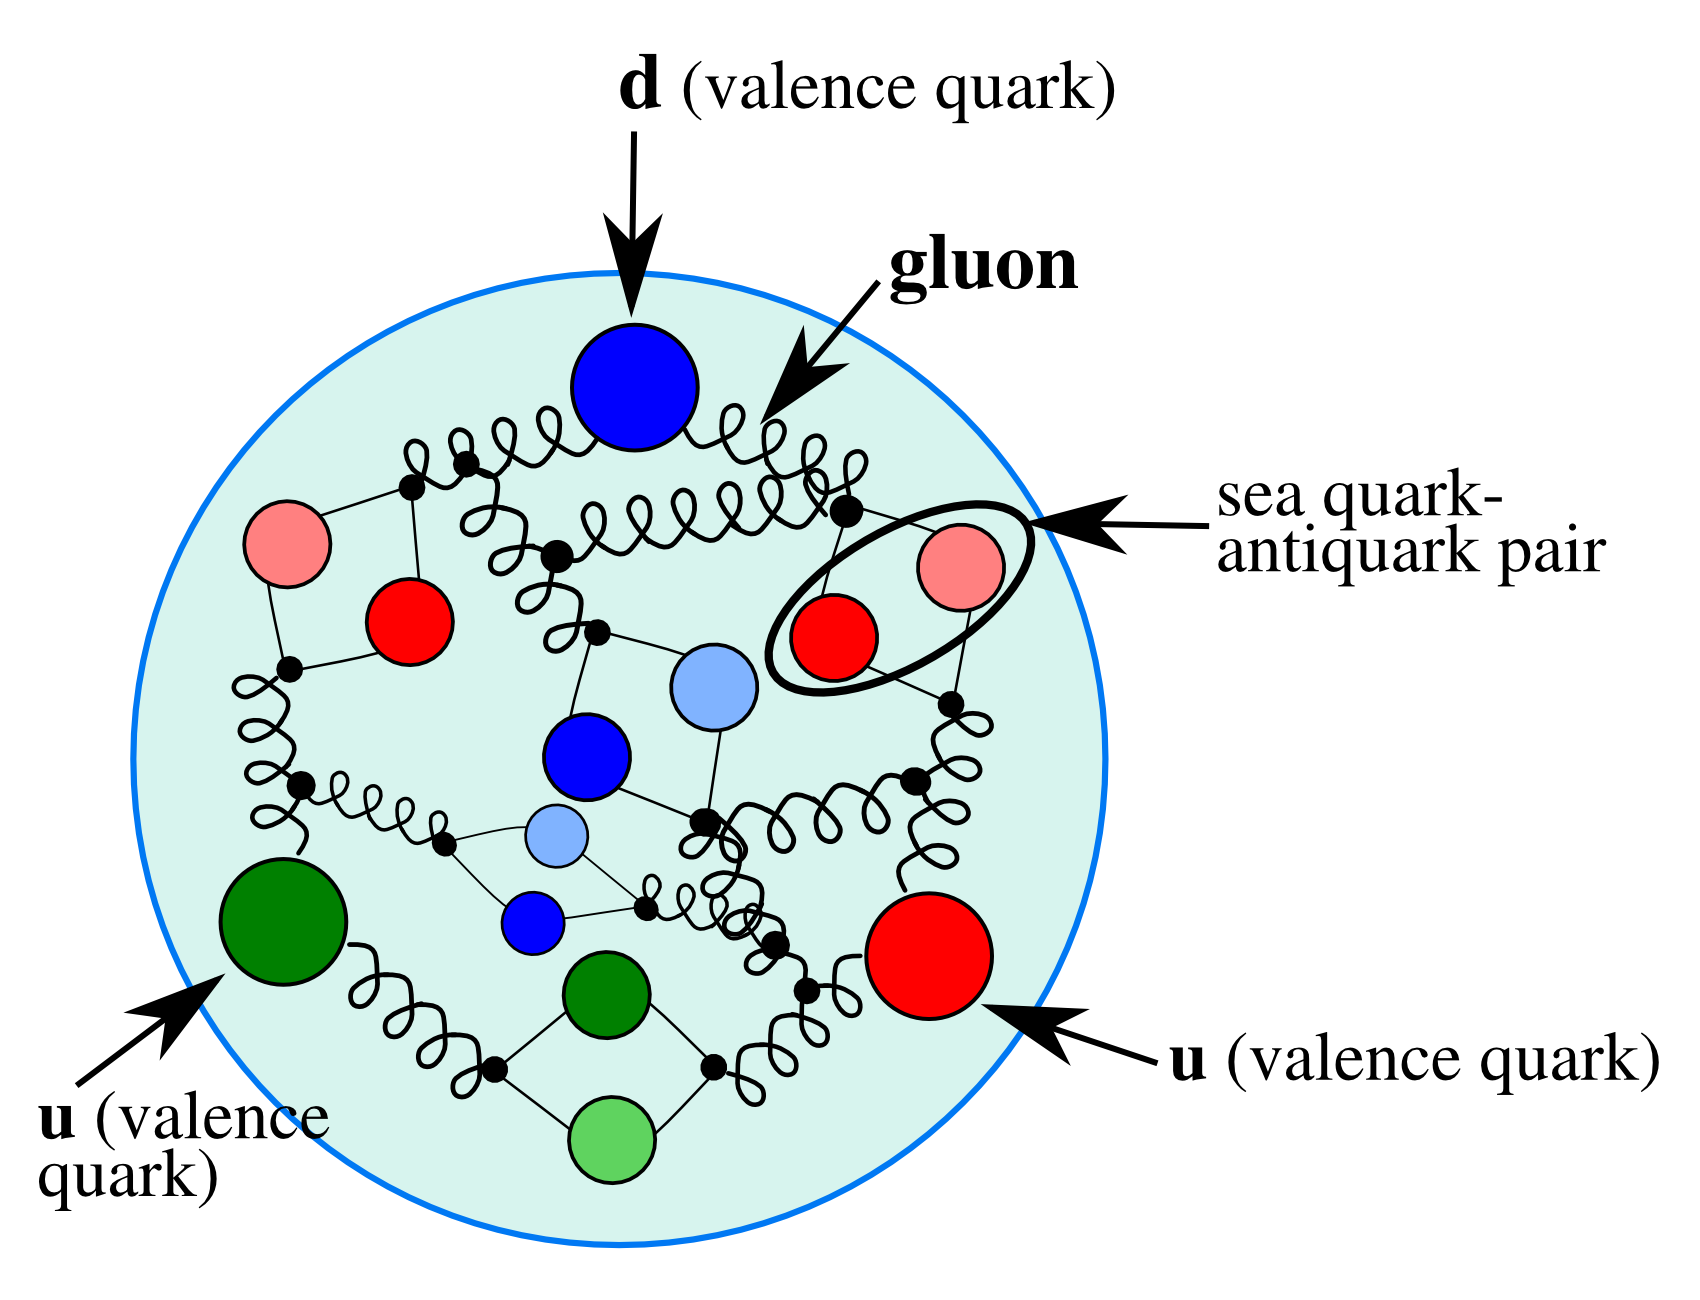
\includegraphics[width=0.45\textwidth]{../figs/Intro/protonStructure.png}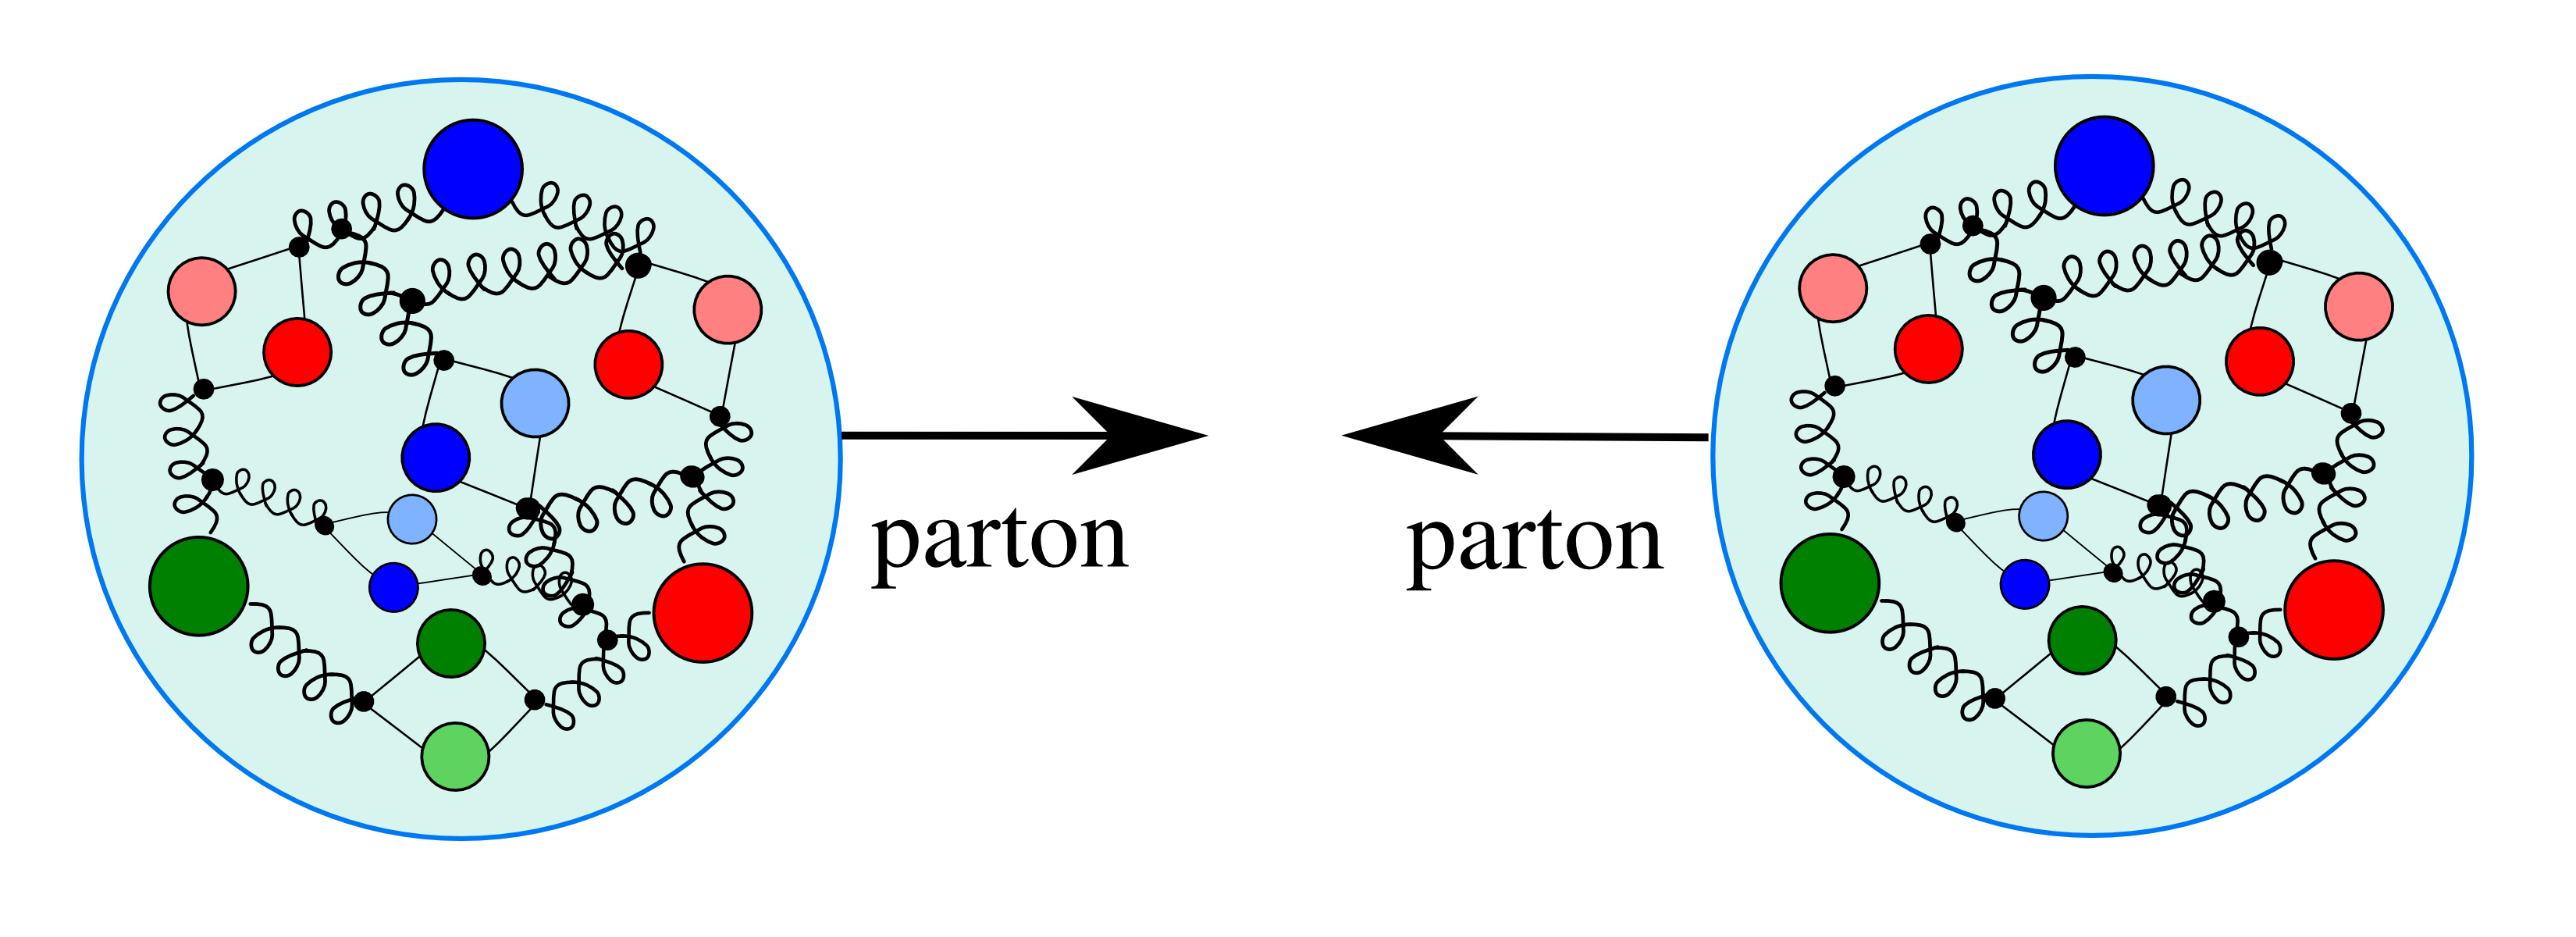
\includegraphics[width=0.45\textwidth]{../figs/Intro/ppCollision.png}}
    \caption{The proton structure (left) and the proton-proton collision (right).}
    \label{fig:ppCollision}
  \end{center}
\end{figure}

\begin{figure}[htb]
  \begin{center}
    {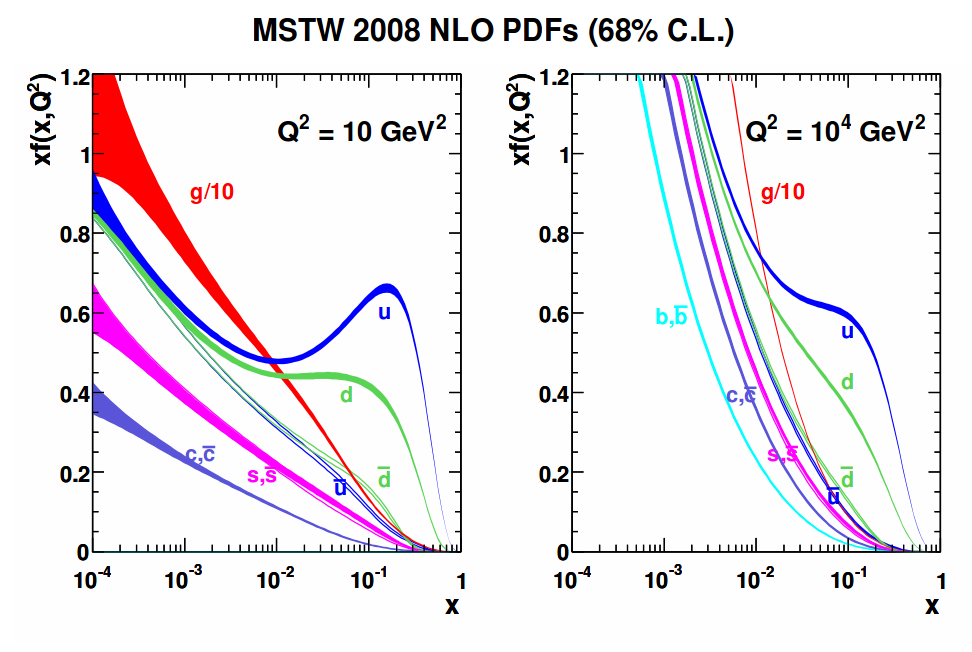
\includegraphics[width=0.85\textwidth]{../figs/Intro/pdfs.png}}
    \caption{Parton distribution functions~\cite{ref_PDG}.}
    \label{fig:pdfs}
  \end{center}
\end{figure}

For large $Q^2$ and $x$ gluon-gluon interactions have the largest probabilities to occur (Fig.~\ref{fig:pdfs}). However, gluons do not couple directly to a $W$ boson, thus, in the $W\gamma$ measurement we are mostly interested in quark-antiquark pairs which would have a total charge corresponding to the charge of a $W$ boson ($\pm 1$). Since we have $u$ and $d$ as valence quarks and we know that the probability to couple to the same generation quark in charged weak interactions is the highest, most of the $W$ bosons are created by $u\bar{d}$ and $d\bar{u}$ pairs however other $q\bar{q'}$ combinations with the total charges of $\pm 1$ are also possible. %As we look for events containing $W\gamma$ we also have other events mimicking our process. Such background events can be produced by any pair of partons.


% ADD FIGURE WITH PDFs LIKE IN THE PRESENTATION


%\subsection{Open Questions of the Standard Model}


While the SM is an accurate description of all particle physics experimental results, there are certain phenomena which are not included into the SM. In this subsection we discuss some of them.\\

The gravitational interactions do not fit into the SM. It is the open question whether the quantum theory of gravity is possible and whether there is a mediator of the gravitational interactions. Also, it is not known why the gravitational force is so much weaker than the other forces. One possible explanation comes from a theory which predicts extra spatial dimensions beyond the three we experience (e.g. the string theory). In this case, it is possible that the gravitational force is shared with other dimensions and only a fraction is available in our three dimensions.\\

Another mystery of the universe is its composition: it is known from the studies of the gravitational effects that our universe consists of dark energy by 68\%, of dark matter by 27\% and of baryon matter only by 5\%~\cite{ref_NASA}. The dark energy resists the gravitational attraction and accelerates the expansion of the universe, and is not detectable by any effects except gravitational. The understanding of dark energy is a question of general relativity rather than particle physics. The dark matter, however, likely consists of particles and therefore is a subject of particle physics. It does not radiate and that is why it cannot be detected by telescopes. The nature of the dark matter is not known but its constituents must be very stable to remain since the Big Bang. The theory of the supersymmetry which is unifying fundamental particles and mediators predicts many of new heavy particles and the lightest supersymmetric particle, the neutralino, is a good candidate for dark matter.\\

One more open question is the reason for the matter/antimatter asymmetry. Matter and antimatter should have been created in the same amount at the moment of the Big Bang. Most of it has annihilated but because of asymmetry, there was more matter than antimatter which led to the state of the Universe we observe now. There is a phenomenon of the CP-violation in weak interactions observed and described which predicts the asymmetry at a certain level. However, the effect of the CP-violation is not large enough to account for the observed amount of the matter and, therefore, the total matter/antimatter asymmetry remains unexplained. \\

The measurement of the photon transverse momentum spectrum ($P_T^{\gamma}$) of the $W\gamma$ process has a goal to both test the SM and search for the BSM physics. The low $P_T^{\gamma}$ region is not expected to be affected by any new physics and must agree well with the SM predictions while the high $P_T^{\gamma}$ region may indicate an existence of new physics if there is an enhancement over the SM predictions. The excess would be indirect evidence of the BSM particles like supersymmetric particles or additional gauge bosons which could be part of the explanation of the dark matter presence or difference in magnitudes of different interactions. More theoretical details about the SM description of W$\gamma$ process as well as possible BSM physics are given in Ch.~\ref{sec:WgAbout}. \\   

%Grand unification and super unification


 % 7-20 pages
\subsection{Fundamental Particles and Interactions}
\label{sec:Intro_FundParticles}

The SM describes interactions of elementary particles. There are four fundamental interactions: electromagnetic, strong, weak and gravitational. The gravity is not included into the SM but its effect on particles is negligible compared to the other forces which makes it possible to develop a theory of the particle physics and conduct experiments even without having the gravity included into the model.\\ 

All fundamental elementary particles in the SM can be split into three categories by their spins. There are fermions which possess spin s=1/2, there are gauge bosons which are vector particles (s=1) and there is the Higgs boson which is a scalar particle (s=0). \\

The fermions are arranged into three generations, each generation consists of a quark with charge Q=$+$2/3(up, charm, and top quarks), a quark with Q=$-$1/3 (down, strange, and bottom quarks), a charged lepton with Q=$-$1 (electron, muon, and tau-lepton) and a neutrino (electron, muon, and tau neutrinos) which is electrically neutral. Each quark can carry any of three colors: red, blue, or green. Additionally, each fermion has its antiparticle. Therefore, the total number of fundamental fermions is $(6 ($leptons$)+6 ($quarks$) \cdot 3 ($colors$) ) \cdot 2 ($to~include~antiparticles$) = 48$.\\ 

Corresponding particles in different generations have the same charges, spins and interaction properties but masses of particles increase with a generation. These mass differences lead to different decay properties because a particle A can decay to particles B and C only if the mass of A $m_A > m_B + m_C$. Thus, an electron is a stable particle, a muon decays as $\mu^- \rightarrow e^- + \bar{\nu_e} + \nu_\mu$, a tau-lepton, as the heaviest charged lepton, has the largest number of decay channels amongst the charged leptons: $\tau^- \rightarrow \mu^- + \bar{\nu_\mu} + \nu_\tau$, $\tau^- \rightarrow e^- + \bar{\nu_e} + \nu_\tau$,  $\tau^- \rightarrow \nu_\tau +$ quarks. \\

In addition to fermions, the SM includes gauge bosons which are interaction mediators. They are called mediators because fermions interact with each other by exchanging them. For example, two charged fermions can interact with each other by exchanging a photon. Such interaction is called electromagnetic interaction and a photon is a mediator for the electromagnetic interaction. Similarly, a gluon is a mediator for the strong interactions, and W$^{\pm}$ and Z$^0$ bosons are mediators for the weak interactions. W$^{\pm}$ and Z$^0$ bosons are massive while a photon and a gluon are massless particles. \\

The last SM particle is the Higgs boson. The Higgs boson is a scalar neutral particle which is playing a critical role in the electroweak symmetry breaking. The Higgs mechanism describes how $W$ and $Z$ bosons become massive particles.\\

All the particles are summarized in Fig. \ref{fig:SMtable}. These and only these fundamental particles and their antiparticles have been discovered by now. However, there are many composite particles which are called hadrons. Hadrons can consist of three quarks (baryons), quark and antiquark (meson), or three antiquarks (antibaryons). Hadrons always possess an integer charge.\\

Most of the particles are short-lived and decay within microseconds. The only stable particles are protons and antiprotons, electrons and positrons, neutrinos and antineutrinos, photons, and, in some sense, gluons. However, if a particle cannot decay, it does not mean that it would live forever. There are many different kinds of reactions in which particles can disappear. Antiprotons and positrons would immediately annihilate with protons and electrons, photons can be absorbed by charged particles, electrons and protons can scatter to produce neutrons and neutrinos and many other reactions are possible.\\ 

In this dissertation a process is studied where quark and antiquark interact to produce a $W$ boson which then decay as $W^\pm \rightarrow e^\pm \nu_e(\bar{\nu_e})$ or $W^\pm \rightarrow \mu^\pm \nu_\mu(\bar{\nu_\mu}) $. A photon is radiated off a quark or antiquark, a charged lepton or a $W$ boson. The most interesting mechanism out of three is a radiation from a $W$ boson because this is the triple gauge coupling where we potentially can have a new physics. Therefore, the focus of this study is an interaction between a photon and a $W$ boson however many other SM particles are relevant too. Thus, a charged lepton and a neutrino appear as the final state particles, a quark and an antiquark appear as initial state particles and all fundamental particles except the Higgs boson participate in various background processes. Subsections \ref{sec:Intro_Electroweak}-\ref{sec:Intro_ppCollisions}, chapter \ref{sec:WgAbout} and \cite{ref_Griffiths} describe particle interactions in more details.\\


\begin{figure}[htb]
  \begin{center}
    {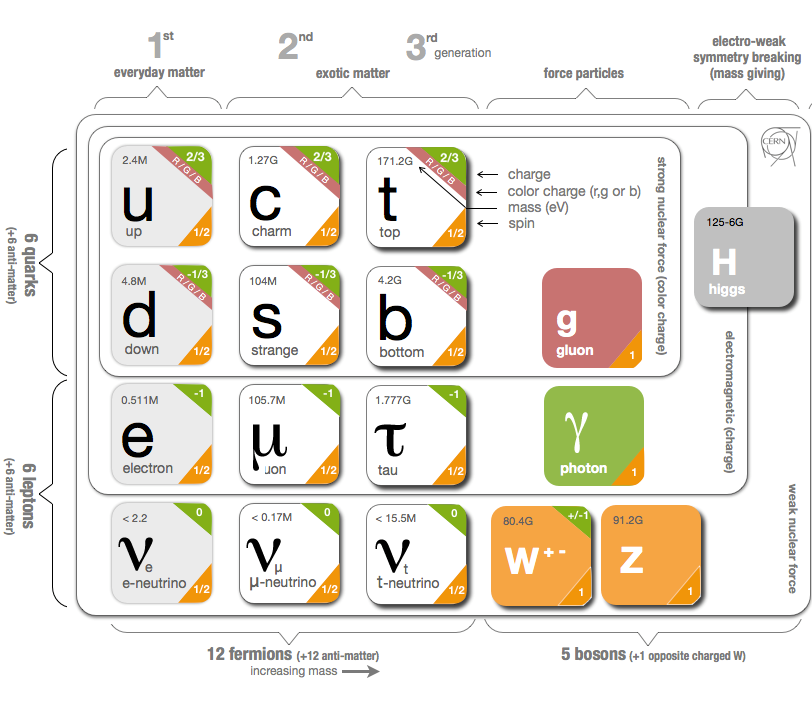
\includegraphics[width=0.90\textwidth]{../figs/Intro/StandardModel.png}}
    \caption{Standard Model Particles and Interations. Source of the figure: \cite{ref_fig_SM}.}
    \label{fig:SMtable}
  \end{center}
\end{figure}






\subsection{Electroweak Interactions}
\label{sec:Intro_Electroweak}

\begin{figure}[htb]
  \begin{center}
    {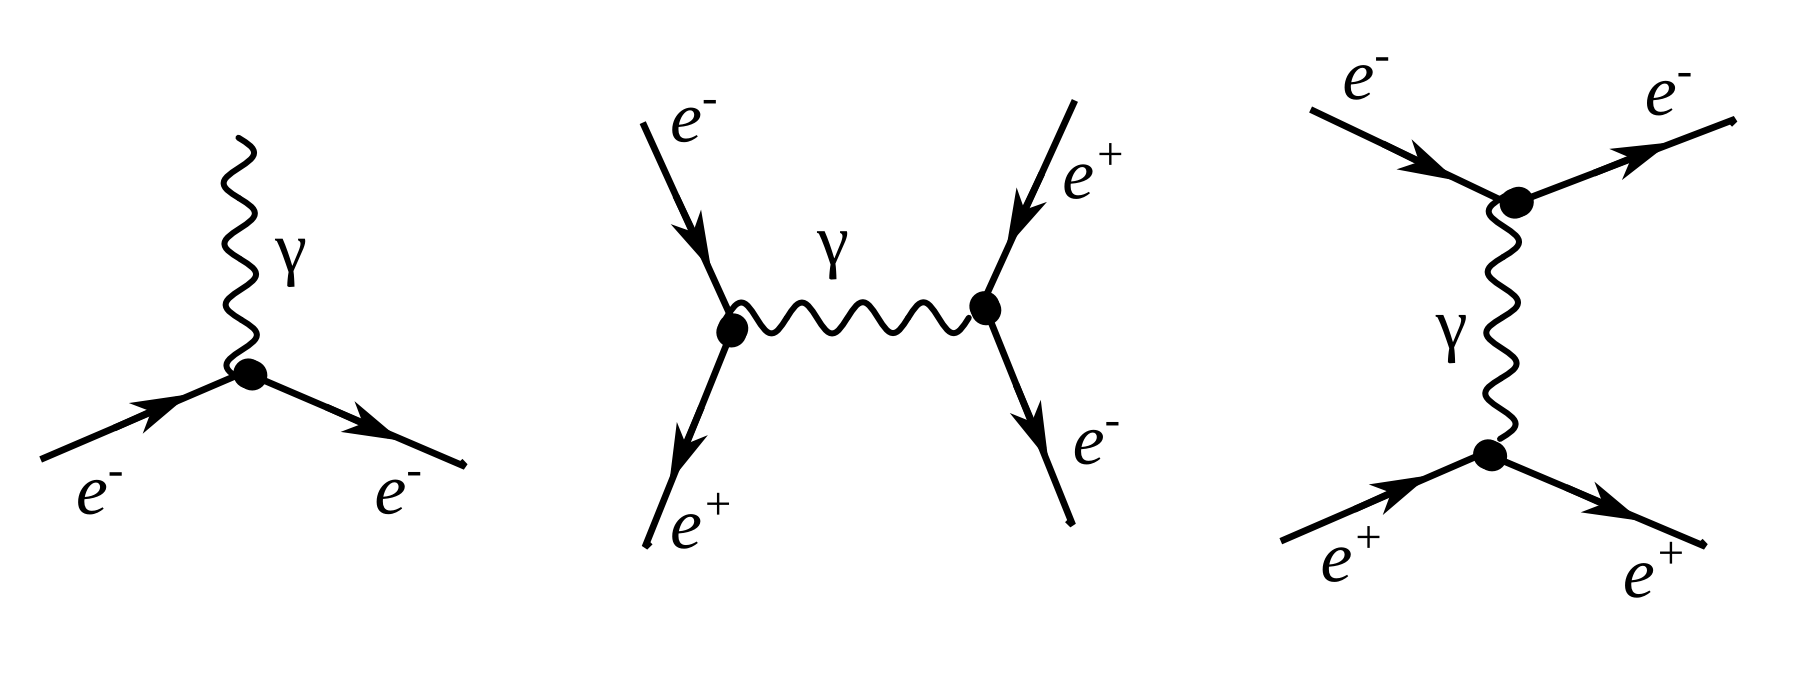
\includegraphics[width=0.90\textwidth]{../figs/Intro/feynmEM.png}}
    \caption{Electromagnetic interations}
    \label{fig:feynmEM}
  \end{center}
\end{figure}

\begin{figure}[htb]
  \begin{center}
    {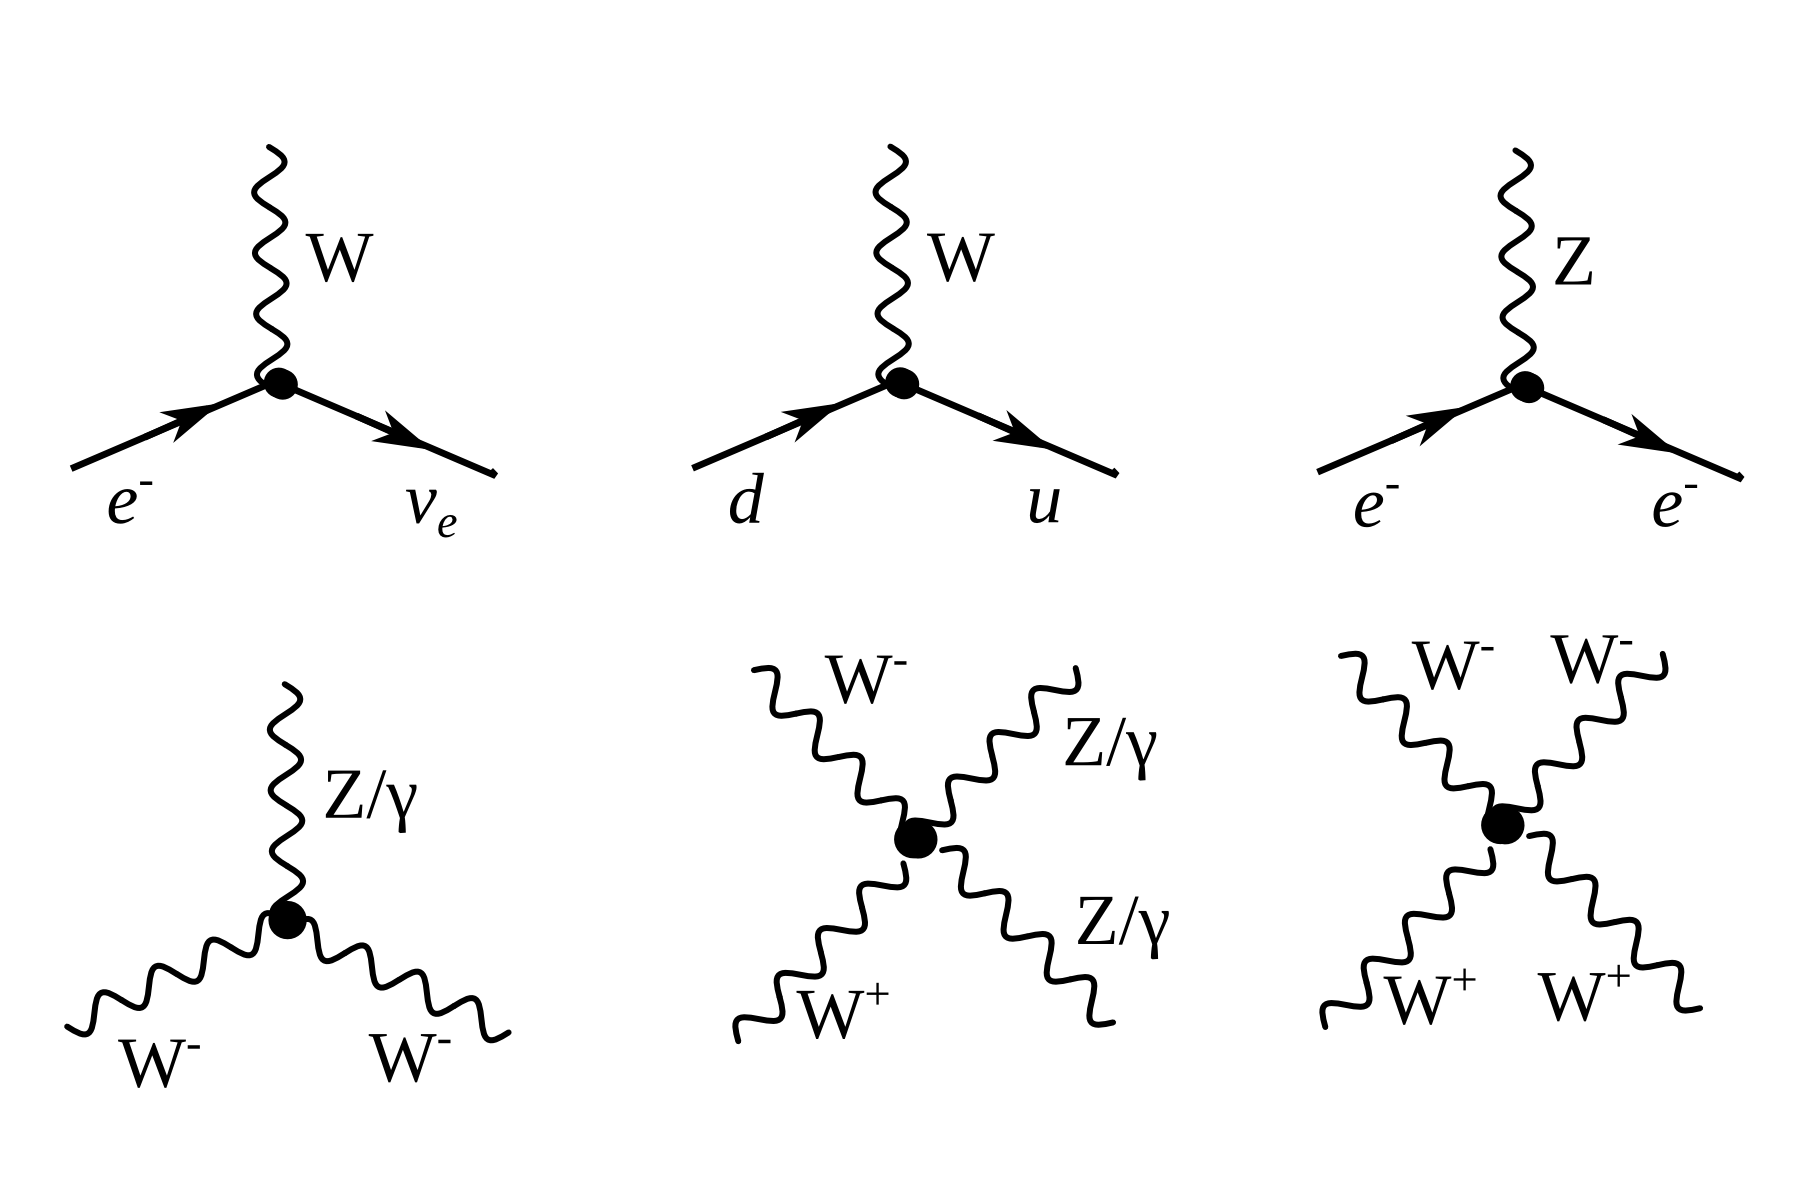
\includegraphics[width=0.90\textwidth]{../figs/Intro/feynmW.png}}
    \caption{Weak interations}
    \label{fig:feynmW}
  \end{center}
\end{figure}

All electrically charged particles participate in electromagnetic interactions. Photon, the mediator of the electromagnetic interactions, is a spin-one electrically neutral massless particle. All electromagnetic interactions can be reduced to one elementary process (Fig. \ref{fig:feynmEM}, left). This process reads: an electron enters, radiates or absorbs a photon, and escapes. Although there is an electron is drawn in this figure, it can be any other charged fermion as well. Such elementary process itself is forbidden by the energy conservation law but this element is a base of actual process (for example, Fig. \ref{fig:feynmEM}, middle and right). Such graphical representations of the particle physics processes are called Feynman diagrams. 

As for the weak interactions, there are two kinds of them: neutral (mediated by a Z boson) and charged (mediated by a W boson). Elementary processes with W and Z bosons are shown in Fig. \ref{fig:feynmW}. An electric charge must be conserved at any vertex. Therefore, if a charged lepton enters and radiates a W boson, a neutrino or antineutrino escapes (top left in Fig. \ref{fig:feynmW}). That is how a W boson interacts with a charged lepton and a neutrino. A lepton flavor number is always conserved in this interaction (Tab. \ref{tab:LeptonFlavorNumber}). 

 \begin{table}[h]
  \begin{center}
  \caption{ Lepton Flavor Number}
  \begin{tabular}{|c|c|c|c|}
     particles & $L_e$ & $L_{\mu}$ & $L_{\tau}$ \\ \hline
     $e^-,\nu_e$ &  +1  &  0  &  0  \\ \hline 
     $e^+, \bar{\nu_e}$ &  -1  &  0  &  0  \\ \hline 
     $\mu^-,\nu_{\mu}$ &  0  &  +1  &  0  \\ \hline 
     $\mu^+, \bar{\nu_{\mu}}$ &  0  &  -1  &  0  \\ \hline 
     $\tau^-,\nu_{\tau}$ &  0  &  0  &  +1  \\ \hline 
     $\tau^+, \bar{\nu_{\tau}}$ &  0  &  0  &  -1  \\ \hline 
  \end{tabular}
  \label{tab:LeptonFlavorNumber}
  \end{center}
\end{table}

From top middle diagram in Fig. \ref{fig:feynmW} we see that if a quark with Q=-1/3 enters, then a quark with Q=+2/3 escapes and, therefore, the flavor of the quarks has changed. The charged weak interaction is the only interaction which changes a quark flavor. The probability of each of three quarks with Q=+2/3 to be born is determined by the Cabibbo–Kobayashi–Maskawa matrix and is the highest for the quark of the same generation as an initial state quark (in this particular case, d is the initial state quark and u has the highest probability to be produced after an interaction with a W boson but c and t can also be produced if there is enough energy).

The right top diagram in Fig. \ref{fig:feynmW} is an emission of a Z boson off a fermion line. An electron is shown here as an example however it also could be any lepton, antilepton, quark or antiquark. All the same diagrams are possible with a photon instead of a Z boson except diagrams with neutrinos and antineutrinos.

The bottom diagrams in Fig. \ref{fig:feynmW} show self-coupling of a W boson, its interaction with Z boson and its electromagnetic radiation of a photon. WWZ, WW$\gamma$, WWZZ, WWZ$\gamma$, WW$\gamma\gamma$ and WWWW vertices are all possible in the SM.

Electromagnetic and weak interactions are unified by the electroweak theory. The mathematical formalism describing these two kinds of interactions is very similar. The difference between a photon and a Z boson is that a Z boson is massive and it can produce a neutrino-antineutrino pair or be scattered off a neutrino which a photon can not. The mass of Z boson is 91 GeV and that is why for low energies the probability of an electromagnetic process is much higher that the probability of similar neutral weak process. However, for particles with energies of E$\gg$91 GeV the mass of the Z boson can be neglected and these probabilities become the same. 

\subsection{Strong Interactions}
\label{sec:Intro_QCD}

\begin{figure}[htb]
  \begin{center}
    {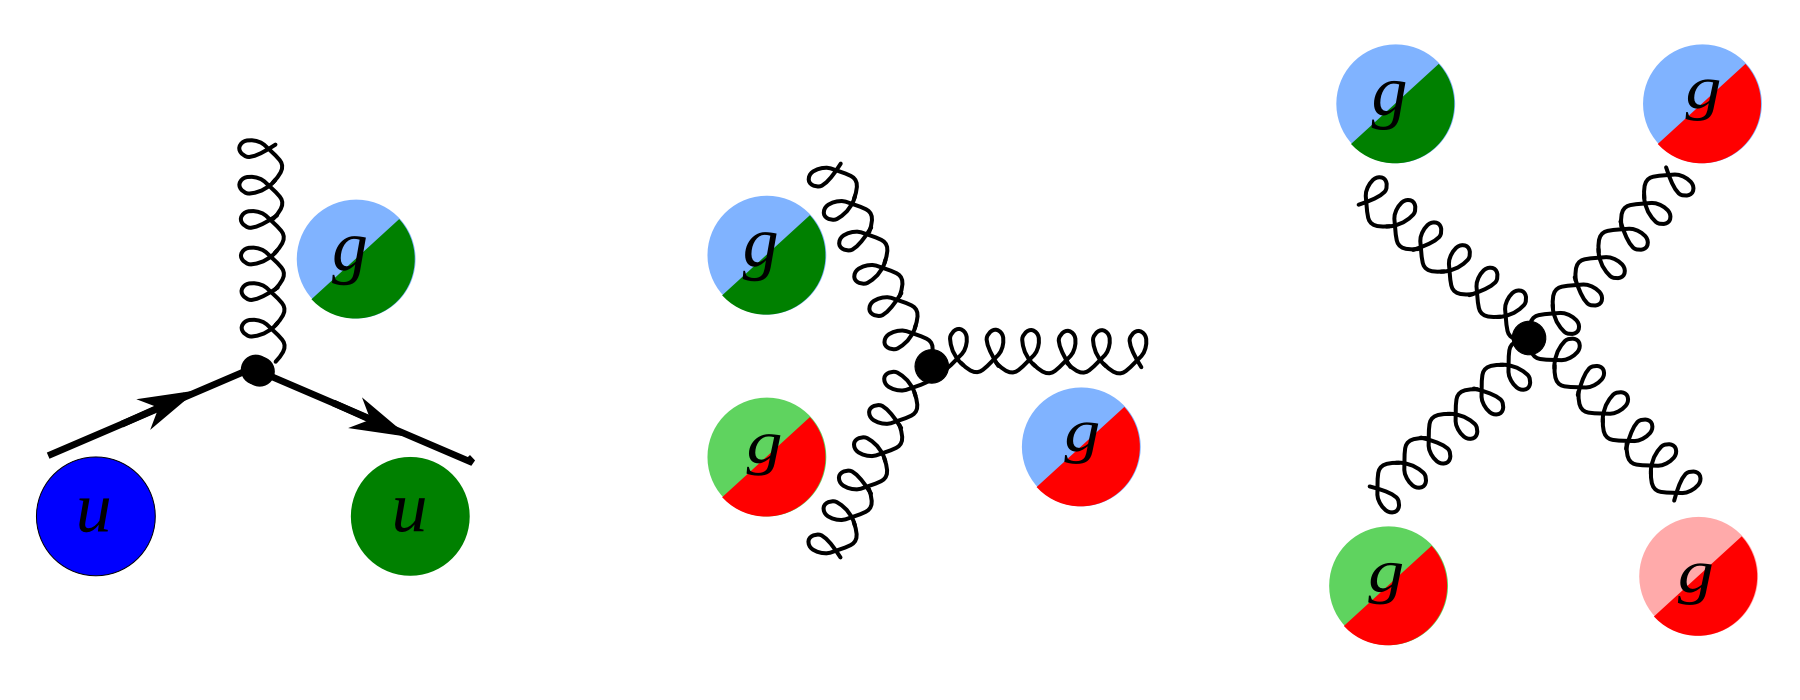
\includegraphics[width=0.80\textwidth]{../figs/Intro/feynmStrong.png}}
    \caption{Elementary processes of strong interations}
    \label{fig:feynmStrong}
  \end{center}
\end{figure}


The third fundamental force after the electromagnetic and weak ones is the strong force. The strong force is responsible for glueing protons and neutrons together in the nuclei as well as for forming protons and neutrons themselves. The strong interactions occur by exchanging gluons which are spin-one massless electrically neutral particles.  \\

The elementary strong processes are shown in Fig. \ref{fig:feynmStrong}. There are three elementary processes: $qqg$, $ggg$ and $gggg$, all are involving particles with color charges. Thus, gluons couple to quarks and self-couple. Color charges must be conserved at each elementary process of the strong interaction. Each quark possesses one of three colors at a time, and there are eight types of gluons to cover all possible color exchanges. \\

The coupling constant of the strong interaction depends on a distance between interacting particles: it becomes larger as the distance becomes larger and smaller as the distance becomes smaller. As the distance approaches zero, the coupling constant approaches zero too, and, thus, in the asymptotic limit two quarks located at the same place do not interact. This property is called asymptotic freedom.\\

On the other hand, when the distance between quarks becomes larger, the coupling constant also becomes larger. This property confines quarks to always stay in the color neutral combinations (hadrons), it forbids the existence of free quarks. A combination becomes color neutral when there is the same amount of color and anticolor or if there is the same amount of each of the three colors.  Thus, mesons are comprised of a quark and an antiquark with the opposite color charges, and baryons are comprised of three quarks: red, green and blue one. Examples of baryons include such well-known particles as a proton and a neutron.\\

The asymptotic freedom and the confinment are properties that are specific for strong interactions. The theory of strong interactions is called the QCD which is a quantum field theory invariant under $SU(3)$ color transformations. When the coupling constant is much less than one $\alpha_s \ll 1$, the perturbative approach can be used to compute observables.\\

The W$\gamma$ process being measured in this dissertation is not intended to test QCD, but a good understanding of QCD is essential for performing this measurement because the QCD corrections to the Feynman diagrams of the process are large and has to be taken into account in producing simulation. In addition, QCD describes the dynamics of quarks and gluons within colliding protons and predicts probabilities of one or another quark-antiquark pair to interact. Physics of proton-proton collisions is discussed in the subsection \ref{sec:Intro_ppCollisions}. \\

% Possible QCD corrections include quark-gluon loops at any of three quark lines as well as exchanges of gluons between different quark lines. 

\section{Physics of Proton-Proton Collisions}
\label{sec:Intro_ppCollisions}

Consider a $pp$ collision at LHC. The proton energies are so high that each proton behaves as a complex structure. A proton is a baryon, it consists of three quarks: $uud$. These three quarks are called valence quarks. They interact with each other by exchanging gluons which produce virtual $q\bar{q}$ pairs (Fig.~\ref{fig:ppCollision}). Such virtual quarks are also called sea quarks. 

Any parton, quark, antiquark or gluon, from one proton can interact with any parton from another proton. Probabilities $f_i(x,Q^2)$ of any particular constituent $i$ to interact are described partially by QCD and partially by experimental measurements and depend on the momentum transfer $Q$ and the momentum fraction of a specific parton $x$. These probabilities are called parton distribution functions (PDFs).

\begin{figure}[htb]
  \begin{center}
    {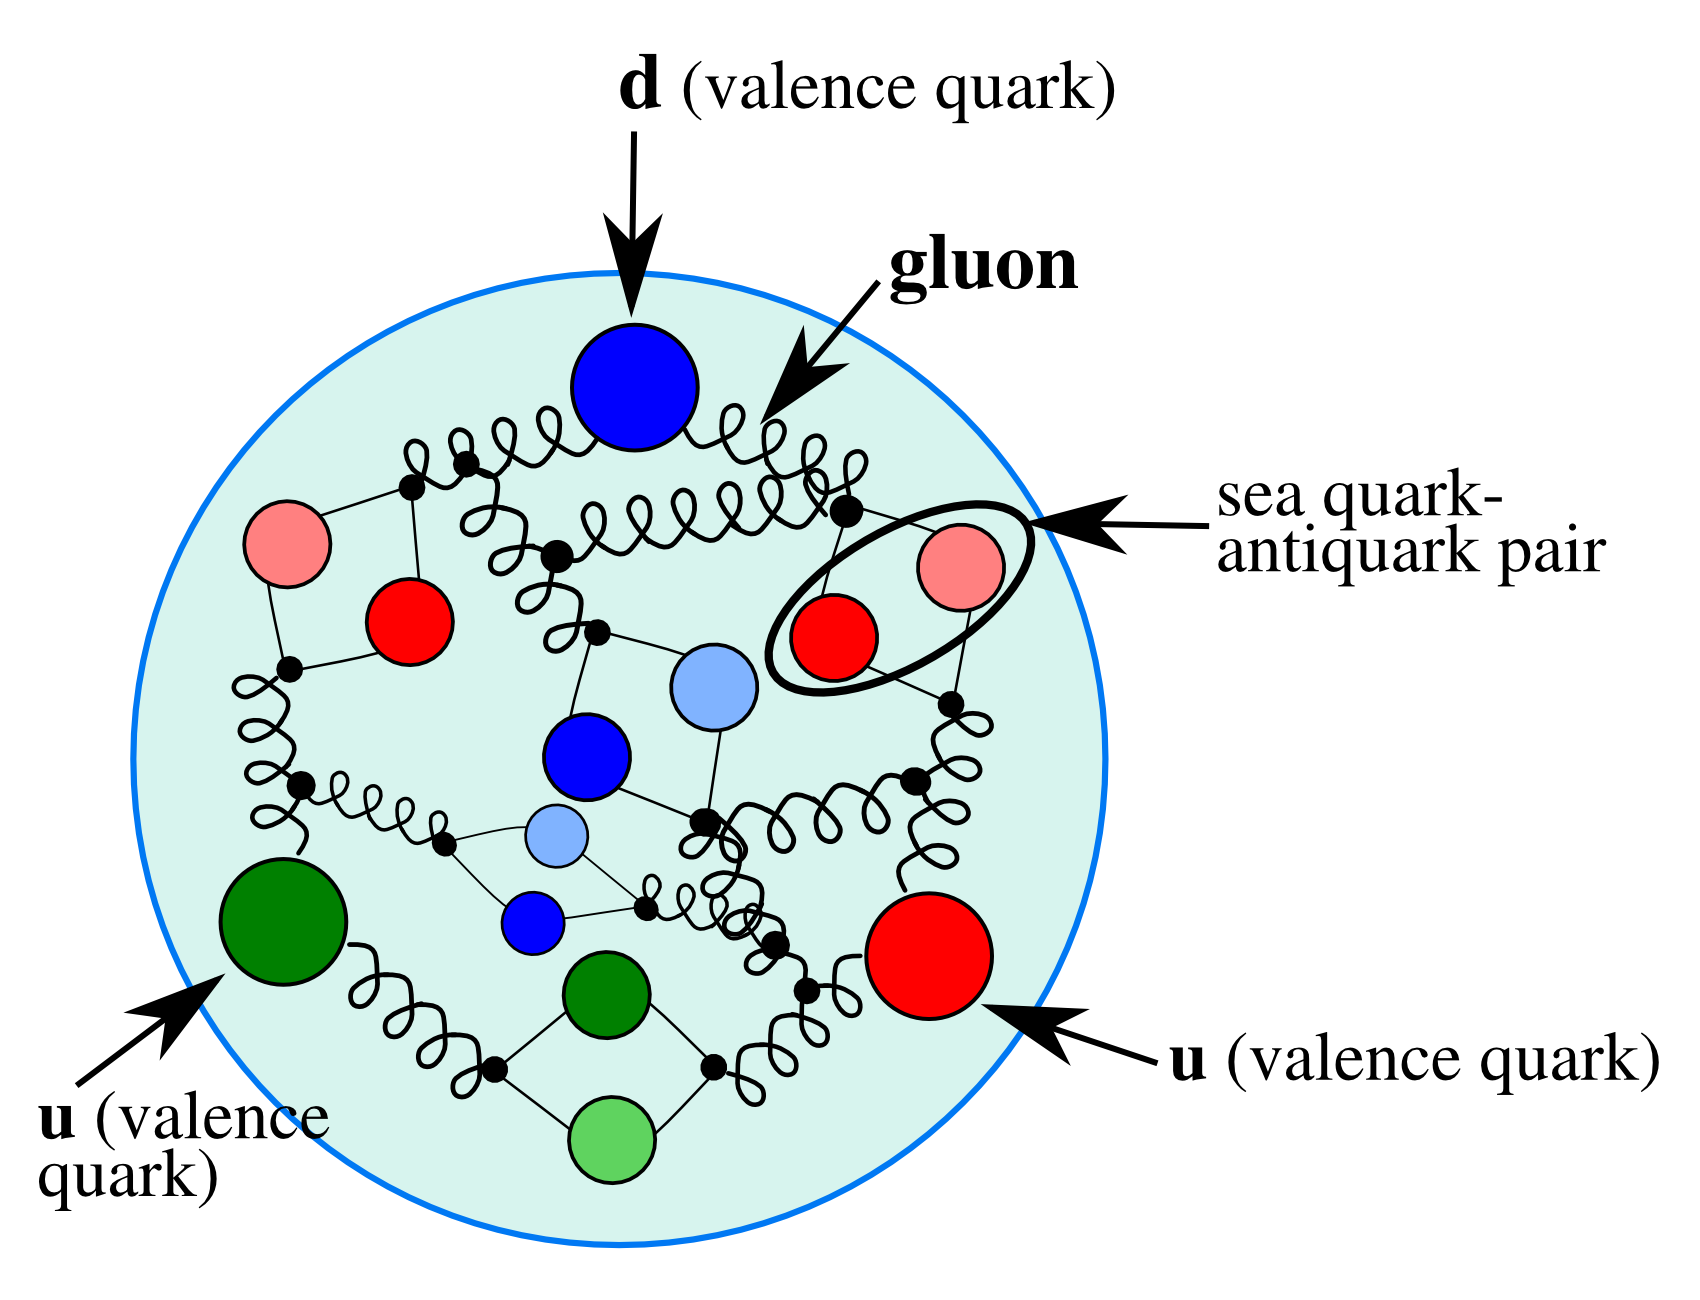
\includegraphics[width=0.45\textwidth]{../figs/Intro/protonStructure.png}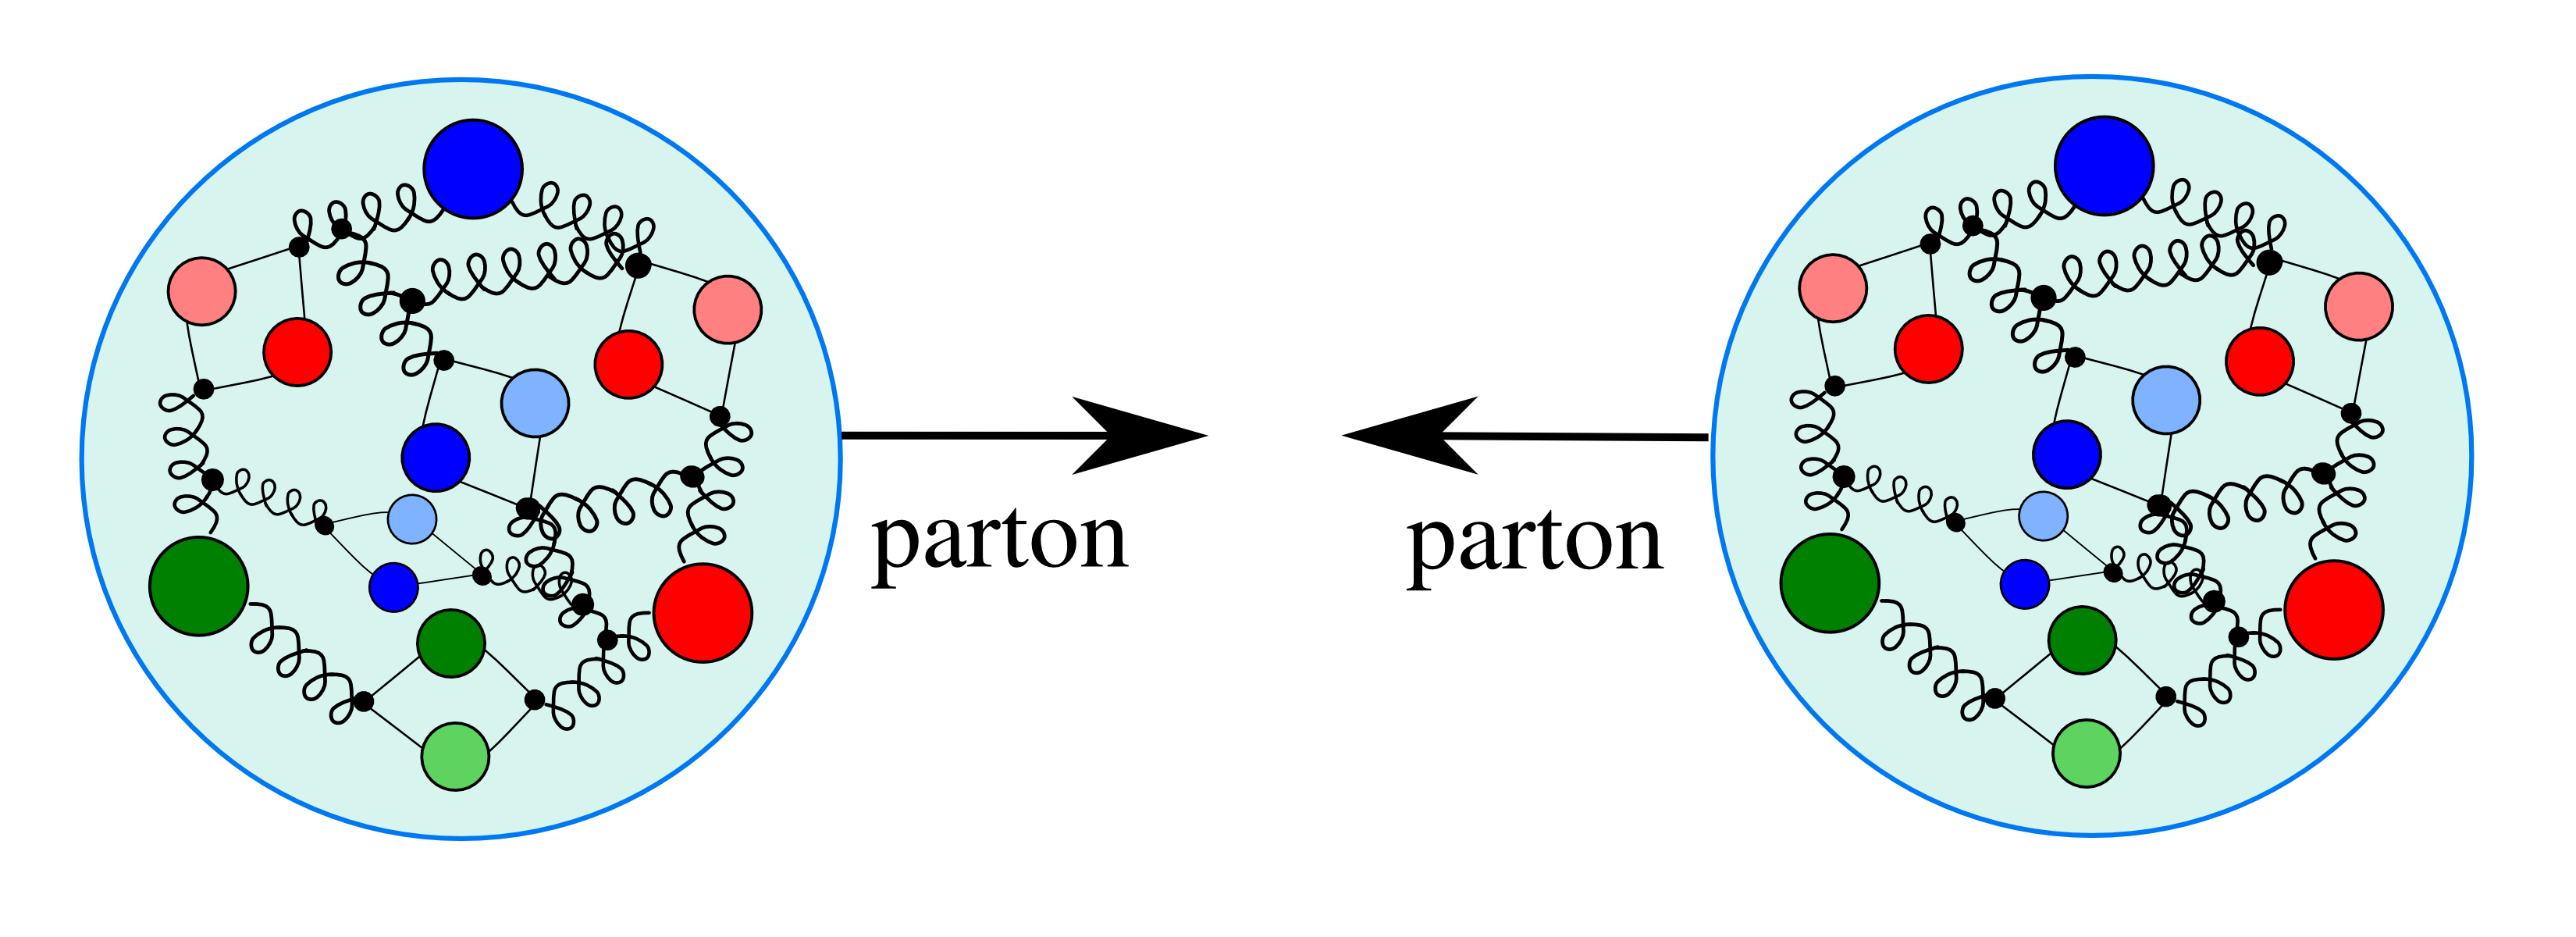
\includegraphics[width=0.45\textwidth]{../figs/Intro/ppCollision.png}}
    \caption{The proton structure (left) and the proton-proton collision (right).}
    \label{fig:ppCollision}
  \end{center}
\end{figure}

\begin{figure}[htb]
  \begin{center}
    {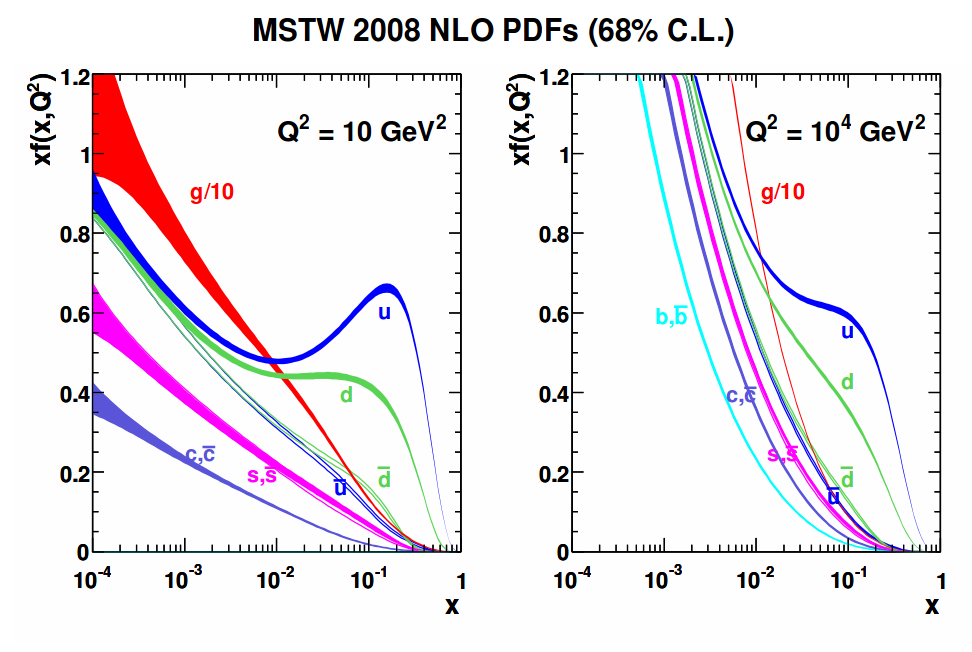
\includegraphics[width=0.85\textwidth]{../figs/Intro/pdfs.png}}
    \caption{Parton distribution functions~\cite{ref_PDG}.}
    \label{fig:pdfs}
  \end{center}
\end{figure}

For large $Q^2$ and $x$ gluon-gluon interactions have the largest probabilities to occur (Fig.~\ref{fig:pdfs}). However, gluons do not couple directly to a $W$ boson, thus, in the $W\gamma$ measurement we are mostly interested in quark-antiquark pairs which would have a total charge corresponding to the charge of a $W$ boson ($\pm 1$). Since we have $u$ and $d$ as valence quarks and we know that the probability to couple to the same generation quark in charged weak interactions is the highest, most of the $W$ bosons are created by $u\bar{d}$ and $d\bar{u}$ pairs however other $q\bar{q'}$ combinations with the total charges of $\pm 1$ are also possible. %As we look for events containing $W\gamma$ we also have other events mimicking our process. Such background events can be produced by any pair of partons.


% ADD FIGURE WITH PDFs LIKE IN THE PRESENTATION


\subsection{Open Questions of the Standard Model}


While the SM is an accurate description of all particle physics experimental results, there are certain phenomena which are not included into the SM. In this subsection we discuss some of them.\\

The gravitational interactions do not fit into the SM. It is the open question whether the quantum theory of gravity is possible and whether there is a mediator of the gravitational interactions. Also, it is not known why the gravitational force is so much weaker than the other forces. One possible explanation comes from a theory which predicts extra spatial dimensions beyond the three we experience (e.g. the string theory). In this case, it is possible that the gravitational force is shared with other dimensions and only a fraction is available in our three dimensions.\\

Another mystery of the universe is its composition: it is known from the studies of the gravitational effects that our universe consists of dark energy by 68\%, of dark matter by 27\% and of baryon matter only by 5\%~\cite{ref_NASA}. The dark energy resists the gravitational attraction and accelerates the expansion of the universe, and is not detectable by any effects except gravitational. The understanding of dark energy is a question of general relativity rather than particle physics. The dark matter, however, likely consists of particles and therefore is a subject of particle physics. It does not radiate and that is why it cannot be detected by telescopes. The nature of the dark matter is not known but its constituents must be very stable to remain since the Big Bang. The theory of the supersymmetry which is unifying fundamental particles and mediators predicts many of new heavy particles and the lightest supersymmetric particle, the neutralino, is a good candidate for dark matter.\\

One more open question is the reason for the matter/antimatter asymmetry. Matter and antimatter should have been created in the same amount at the moment of the Big Bang. Most of it has annihilated but because of asymmetry, there was more matter than antimatter which led to the state of the Universe we observe now. There is a phenomenon of the CP-violation in weak interactions observed and described which predicts the asymmetry at a certain level. However, the effect of the CP-violation is not large enough to account for the observed amount of the matter and, therefore, the total matter/antimatter asymmetry remains unexplained. \\

The measurement of the photon transverse momentum spectrum ($P_T^{\gamma}$) of the $W\gamma$ process has a goal to both test the SM and search for the BSM physics. The low $P_T^{\gamma}$ region is not expected to be affected by any new physics and must agree well with the SM predictions while the high $P_T^{\gamma}$ region may indicate an existence of new physics if there is an enhancement over the SM predictions. The excess would be indirect evidence of the BSM particles like supersymmetric particles or additional gauge bosons which could be part of the explanation of the dark matter presence or difference in magnitudes of different interactions. More theoretical details about the SM description of W$\gamma$ process as well as possible BSM physics are given in Ch.~\ref{sec:WgAbout}. \\   

%Grand unification and super unification



\section{W$\gamma$ Production Theory and Former Experimental Results} % 5-10 pages
\label{sec:WgAbout}
\subsection{Electroweak Theory of the Standard Model}
\label{sec:WgAbout_SMEWK}

%Pich, 1

The SM is a gauge theory invariant under the local $SU(3)_C \times SU(2)_L \times U(1)_Y$ transformation. $SU(3)_C$ stands for color transformations and, therefore, the $SU(3)_C$-invariant Lagrangian describes QCD: color interactions of quarks and antiquarks. The requirement to satisfy the gauge invariance generates eight massless gluons, and the non-abelian nature of the $SU(3)$ group generates self-interactions of gluons including three-gluon and four-gluon vertices.\\

The Lagrangian based on the $SU(2)_L \times U(1)_Y$ symmetry descibes unified theory of electroweak interactions. The requirement of the local gauge invariant generates four massless vector bosons which are mediators of electromagnetic and weak interactions. The non-abelian structure of $SU(2)$ group introduces gauge boson couplings just like self-interactions of gluons appear in QCD.\\ 

While the vector bosons are generated by the gauge theory formalism to be massless, it is experimentally known that mediators of weak interactions are heavy particles with masses $M_W=80$~GeV and $M_Z=91$~GeV. To introduce these masses, the electroweak symmetry has to be spontaneously broken to the QED symmetry group $U(1)$:\\

$SU(2)_L \times U(1)_Y \rightarrow U(1)_{QED}$\\

The Spontaneous Symmetry Breaking (SSB) introduces an additional particle into the SM: a Higgs boson ($H$) and generates masses for $W$ and $Z$ bosons. A photon is a massless particle, therefore, $U(1)_{QED}$ symmetry remains unbroken and a photon does not couple to a Higgs boson.\\

The Lagrangian transformations of the SM are described in \cite{ref_Pich} for QED, QCD, unified electroweak force and the Higgs mechanism. The measurement in this dissertation provides a test for the electroweak sector of the SM, thus we will repeat here the theoretical path from the Lagrangians of free particles to the accomodation of the electroweak gauge bosons including their self-couplings to explain better what model is tested.\\

%Pich, 3.1
It is experimentally known that dynamics of weak interactions depends on particle's helicity \cite{ref_Griffiths}. Thus, only left-handed fermions and only right-handed antifermions couple to a $W$ boson. A $Z$ boson couples to both left-handed and right-handed fermions and antifermions except neutrinos but with different strength while photon-fermion couplings do not depend on helicity but on electric charge only. As for the neutrinos, only left-handed neutrinos and right-handed antineutrinos found to couple to a $Z$ boson, therefore, right-handed neutrinos and left-handed antineutrinos were not found to participate in any SM interactions and even their existence is under the question.\\

Given different properties of left-handed and right-handed particles, they are treated differently by the electroweak theory. $SU(2)$ doublets are introduced for the wave functions of left-handed particles while $SU(2)$ singlets are introduced for the wave functions of right-handed particles. Eq.~\ref{eq:psi_for_quarks} and Eq.~\ref{eq:psi_for_leptons} show wave functions for the first generation fermions, however wave functions for the other two generations are constructed the same way.\\ 
 
%Pich 3.2

\begin{equation}\label{eq:psi_for_quarks}
\psi_1(x)=\begin{pmatrix} u \\ d' \end{pmatrix}_L \text{, } \psi_2(x)=u_R \text{, } \psi_3(x)=d'_R \text{.}
\end{equation}

\begin{equation}\label{eq:psi_for_leptons}
\psi_1(x)=\begin{pmatrix} \nu_e \\ e^- \end{pmatrix}_L \text{, } \psi_2(x)=\nu_{eR} \text{, } \psi_3(x)=e^-_R \text{. }
\end{equation}

The state $d'$ is a mixture of $d$, $c$ and $b$ quark's wave functions and is deternimed by the Cabbibo-Kobayashi-Maskawa matrix \cite{ref_Pich}:

\begin{equation}
  \begin{pmatrix} d' \\ c' \\ b' \end{pmatrix} = V
  \begin{pmatrix} d \\ c \\ b \end{pmatrix}
\end{equation}

Consider the free Lagrangian:\\

\begin{equation}\label{eq:L_free}
L_0 = \sum_{j=1}^{3} i \bar{\psi_j}(x) \gamma^\mu \partial_\mu \psi_j(x) 
\end{equation}

where $\gamma^\mu$ are Dirac matrices \cite{ref_Griffiths}.\\

The wave function $\psi_1$ changes under the $SU(2)_L \times U(1)_Y$ transformations in the following way:\\

\begin{equation}
\psi_1(x) \rightarrow e^{i y_1 \beta} U_L \psi_1(x)
\end{equation}


The wave functions $\psi_{(2,3)}(x)$ are singlets of $SU(2)_L$ and are affected only by $U(1)$ transformations:\\

\begin{equation}
\psi_{(2,3)}(x) \rightarrow e^{i y_{(2,3)} \beta} \psi_{(2,3)}(x)
\end{equation}

The transformation $U_L \equiv e^{i \sigma_i \alpha_i /2}$, $\sigma_i$ are Pauli matrices \cite{ref_Griffiths}, $\alpha_i(x)$ and $\beta(x)$ are arbitrary functions, $y_{(1,2,3)}$ are hypercharges which are named analogous to electric charges in QED.\\

In order to satisfy the local Largangian invariance, partial derivatives in Eq.~\ref{eq:L_free} has to be substituted with covariant derivatives:\\

\begin{equation}
D_\mu \psi_1(x) = [\partial_\mu - i g {\tilde{W}}_\mu(x) - i g' y_1 B_\mu(x) ] \psi_1(x) 
\end{equation}

\begin{equation}
D_\mu \psi_{(2,3)}(x) = [\partial_\mu - i g' y_{(2,3)} B_\mu(x) ] \psi_{(2,3)}(x) 
\end{equation}

where ${\tilde{W}}_\mu(x) \equiv \frac{\sigma_i}{2} W_\mu^i(x) = \frac{1}{\sqrt{2}} 
\begin{pmatrix}
\sqrt{2} W_\mu^3 & (W_\mu^1 - i W_\mu^2)/{\sqrt{2}}\\
(W_\mu^1 + i W_\mu^2)/{\sqrt{2}} & -W_\mu^3\\
\end{pmatrix}$.

The Lagrangian becomes:\\ \\

\begin{equation}\label{eq:L_free_covariant}
L_0 \rightarrow L = \sum_{j=1}^{3} i \bar{\psi_j}(x) \gamma^\mu D_\mu \psi_j(x) 
\end{equation}


The Lagrangian $L$ from Eq.~\ref{eq:L_free_covariant} is now invariant under local $SU(2)_L \times U(1)$ transformations. Four vector boson fields appear in $L$: $B_\mu$, $W_\mu^1$, $W_\mu^2$, $W_\mu^3$.  Thus, it is necessary to add terms for kinetic energies of the vector bosons:\\

\begin{equation} \label{eq:L_gauge_kin}
L_{KIN}=-\frac{1}{4}B_{\mu\nu}B^{\mu\nu}-\frac{1}{4}W_{\mu\nu}^i W^{\mu\nu}_i
\end{equation}

where $B_{\mu\nu} \equiv \partial_\mu B_\nu - \partial_\nu B_\mu$, $W_{\mu\nu}^i \equiv \partial_\mu W_\nu^i - \partial_\nu W_\mu^i + g \epsilon^{ijk} W_\mu^j W_\nu^k$\\

Off-diagonal terms of ${\tilde{W}}_\mu$ are wave functions of charged vector bosons $W^{\pm}=W_\mu^1 \mp i W_\mu^2)/{\sqrt{2}}$ while $W_\mu^3$ and $B_\mu$ are neutral fields corresponding to a $Z$ boson and a photon. However, $W_\mu^3$ couples to left-handed fermions and right-handed antifermions only while a $Z$ boson is known to interact with particles of both helicities.\\

Then the neutral electroweak mixing is introduced:\\

\begin{equation}
  \begin{pmatrix} W_\mu^3 \\ B_\mu \end{pmatrix} \equiv
  \begin{pmatrix} \cos \theta_W & \sin \theta_W \\ -\sin \theta_W & \cos \theta_W \end{pmatrix}
  \begin{pmatrix} Z_\mu \\ A_\mu \end{pmatrix}
\end{equation} 

where $\theta_W$ is an electroweak mixing angle, $A_\mu$ is a photon field.\\

Terms involving $A_\mu$ in the electroweak Largangian must be equal to the corresponding terms in QED Lagrangian \cite{ref_Pich}:\\

\begin{equation}\label{eq:L_QED}
L_{QED} = i \bar{\psi}(x) \gamma^\mu \partial_\mu \psi(x) - m \bar{\psi}(x) \psi(x) + e Q A_\mu(x) \bar{\psi}(x) \gamma^\mu \psi(x) - \frac{1}{4} F_{\mu\nu}(x) F^{\mu\nu}(x)
\end{equation}

where $F_{\mu\nu} \equiv \partial_\mu A_\nu - \partial_\nu A_\mu$.

This requirement relates $g$, $g'$, $\theta_W$ and $e$ as $g \sin \theta_W = g' \cos \theta_W = e$ and provides expression for weak hypercharges: $Y = Q - T_3$,\\

where $T_3 = \sigma_3 / 2$, $Q_1 = \begin{pmatrix} Q_{u/\nu} & 0 \\ 0 & Q_{d/e} \end{pmatrix}$, $Q_2 = Q_{u/\nu}$, $Q_3=Q_{d/e}$.\\

Writing $\tilde{W}_\mu$ in Eq.~\ref{eq:L_gauge_kin} explicitely, we will receive TGC and QGC coupling terms: 

\begin{equation} \label{eq:L_TGC_1}
L_{TGC} = -\frac{g}{4}(\partial_\mu W_\nu^i - \partial_\nu W_\mu^i)\epsilon^{ijk}W^{\mu j}W^{\nu k} - \frac{g}{4}\epsilon^{ijk}W_\mu^j W_\nu^k (\partial^\mu W^{\nu i} - \partial^\nu W^{\mu i})
\end{equation}

\begin{equation} \label{eq:L_QGC_1}
L_{QGC} = -\frac{g^2}{4} \epsilon^{ijk} \epsilon^{ilm} W_\mu^j W_\nu^k W^{\mu l} W^{\nu m}
\end{equation}

Substitute $W_\mu^i$ and $B_\mu$ in Eq.~\ref{eq:L_TGC_1} and Eq.~\ref{eq:L_QGC_1} with the wave functions of $W^\pm$, $Z$ and a photon:\\

\begin{equation} \label{eq:EWK_Zg_bosons_mixing}
B_\mu = -\sin \theta_W Z_\mu + \cos \theta_W A_\mu \text{, } W_\mu^3 = \cos \theta_W Z_\mu + \sin \theta_W A_\mu
\end{equation}
\begin{equation} \label{eq:EWK_Zg_bosons_mixing}
W_\mu^1 = \sqrt{2}(W^+ + W^-) \text{, }W_\mu^2 = \sqrt{2}(W^- + W^+)
\end{equation}

we will receive charged TGC and QGC Lagrangians in the forms Eq.~\ref{eq:L_TGC_2} and Eq.~\ref{eq:L_QGC_2} which involve $WWZ$ (Eq.~\ref{eq:L_TGC_2_1}), $WW\gamma$ (Eq.~\ref{eq:L_TGC_2_2}), $WWWW$ (Eq.~\ref{eq:L_QGC_2_1}), $WWZZ$ (Eq.~\ref{eq:L_QGC_2_2}), $WWZ\gamma$ (Eq.~\ref{eq:L_QGC_2_3}), and $WW\gamma\gamma$ (Eq.~\ref{eq:L_QGC_2_4}) interactions.\\


\begin{equation} \label{eq:L_TGC_2}
L_{TGC} = L_{TGC}^{(1)} + L_{TGC}^{(2)}
\end{equation}

\begin{equation} \label{eq:L_TGC_2_1}
L_{TGC}^{(1)} = -ie \cot \theta_W (W^{-\mu\nu} W^{+}_\mu Z_\nu - W^{+\mu\nu} W^-_\mu Z_\nu +W^-_\mu W^+_\nu Z^{\mu\nu}) 
\end{equation}

\begin{equation} \label{eq:L_TGC_2_2}
L_{TGC}^{(2)} = - ie(W^{-\mu\nu}W^+_\mu A_\nu - W^{+\mu\nu}W^-_\mu A_\nu + W^-_\mu W^+_\nu A^{\mu\nu})
\end{equation}

\begin{equation} \label{eq:L_QGC_2}
L_{QGC} = L_{QGC}^{(1)} + L_{QGC}^{(2)} + L_{QGC}^{(3)} + L_{QGC}^{(4)}
\end{equation}

\begin{equation} \label{eq:L_QGC_2_1}
L_{QGC}^{(1)} = -\frac{e^2}{2\sin^2 \theta_W}(W^+_\mu W^{-\mu}W^+_\nu W^{-\nu} - W^+_\mu W^{\mu +} W^-_\nu W^{-\nu})
\end{equation}

\begin{equation} \label{eq:L_QGC_2_2}
L_{QGC}^{(2)} = - e^2 \cot^2 \theta_W (W^+_\mu W^{-\mu} Z_\nu Z^{\nu} - W^+_\mu Z^{\mu} W^-_\nu Z^{\nu})
\end{equation}

\begin{equation} \label{eq:L_QGC_2_3}
L_{QGC}^{(3)} = - e^2 \cot \theta_W (2 W_\mu^+ W^{-\mu} Z_\nu A^{\nu} - W^{+}_\mu Z^\mu W^-_\nu A^\nu - W^{+}_\mu A^\mu W^-_\nu Z^\nu)
\end{equation}

\begin{equation} \label{eq:L_QGC_2_4}
L_{QGC}^{(4)} = - e^2 (W^+_\mu W^{-\mu} A_\nu A^{\nu} - W^+_\mu A^{\mu} W^-_\nu A^{\nu})
\end{equation}

In the measurement of this dissertation we probe $WW\gamma$ coupling.\\

The unified electroweak Lagrangian discussed above involves kinetic energy terms for fermions and gauge bosons as well as interactions of fermions with gauge bosons, TGC, and QGC. However, this Lagrangian does not contain any mass terms.\\

Because left-handed and right-handed wave functions transform differently under the electroweak symmetry, fermion mass terms of $\frac{1}{2} m_f^2 \bar{\psi} \psi$ would not be invariant and, therefore, are forbidden by the $SU(2) \times U(1)$ symmetry requirement. Mass terms for gauge bosons also would violate the Lagrangian invariance just as a photon mass term $\frac{1}{2} m^2 A^\mu A_\mu$ would violate $U(1)$ invariance of $L_{QED}$ \cite{ref_Griffiths}. Therefore, Largangian $L$ in Eq. \ref{eq:L_free_covariant} contains massless particles only.\\

To introduce masses into the electroweak Lagrangian, an $SU(2)_L$ doublet of complex scalar fields $\phi(x)$ is added to the Lagrangian:\\

\begin{equation}\label{eq:H_doublet}
  \phi(x) \equiv \begin{pmatrix} \phi^{(+)}(x) \\ \phi^{(0)}(x) \end{pmatrix}
\end{equation}

By selecting a special gauge of $\phi(x)$ it is possible to spontaneously break electroweak symmetry, generate a new scalar particle, a Higgs boson \cite{ref_Pich}, and introduce mass terms for $W$ and $Z$ bosons and charged fermions through their couplings to the Higgs boson. The strength of the coupling constant is proportional to the square of the particle's mass, therefore, heavier particles are more likel to interact with $H$, and massless particles do not couple to $H$.\\

The mechanism of generating a fermion's mass involve both left-handed and right-handed components of the fermion. If our hypothesis that right-handed neutrinos do not exist is right, then the Higgs mechanism does not generate neutrino masses. However, from the experiments of neutrino oscillations, neutrinos are known to have masses even though they are oreders of magnitude smaller than those of other fermions. Several hypotheses were offered to resolve this contradiction however at the moment the mechanism of neutrinos to acquire masses remain unknown \cite{ref_PDG}.\\


\subsection{Luminosity and Cross Section}




\begin{figure}[htb]
  \begin{center}
    {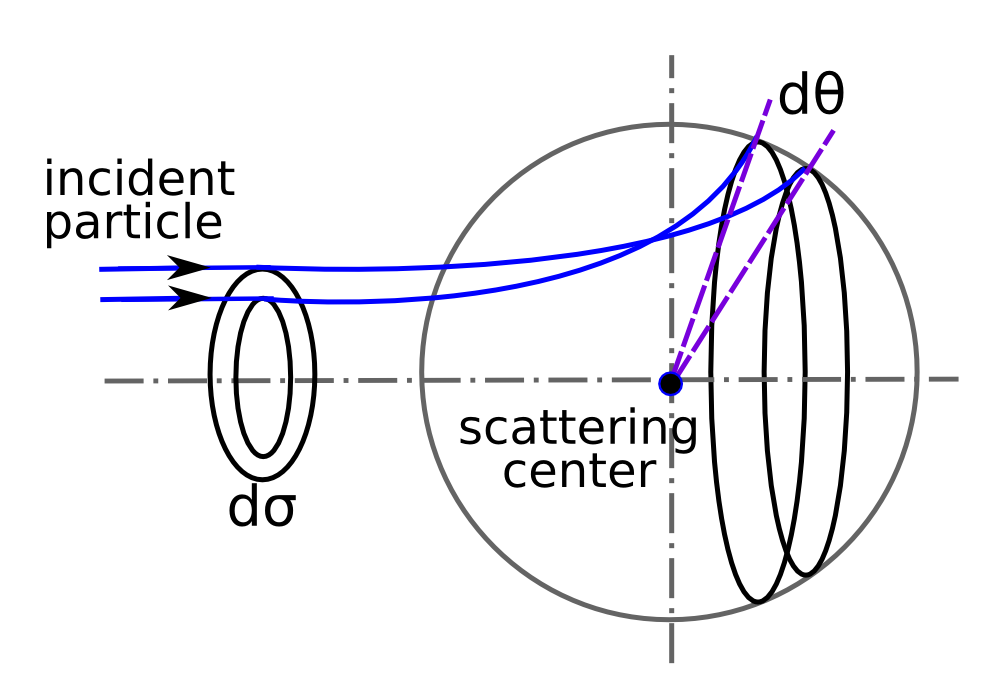
\includegraphics[width=0.70\textwidth]{../figs/WgAbout/CSclassical.png}}
    \caption{Illustration of the differential cross section concept in the classical case}
    \label{fig:CSclassical}
  \end{center}
\end{figure}

In this dissertation we are measuring the total and the differential cross section. Fig. \ref{fig:CSclassical} illustrates the concept of the differential cross section in the classical case. An incident particle must appear within area $d\sigma$ to be scattered off by an angle $d\theta$ by the scattering center. The relashionship between these two quantities would give us the expression for the differential cross section $d\sigma/d\theta$. Integrating over $d\theta$, one would get the total cross section $\sigma$. Differentiating $\sigma$ by any kinematic parameter $X$ of the incident particle would give the expression for the differential cross section $d\sigma/dX$.\\

In particle physics the cross section characterizes the probability of two particles to interact or, more specifically, the probability of two particles to interact to produce the specific final state. For example, the probability of a quark and an antiquark to interact to produce a charged lepton, a neutrino and a photon like in our measurement.\\

Referring to the Fig. \ref{fig:CSclassical}, a number of particles passing through the area $\sigma$ per unit time is $N=L \cdot \sigma$, where L is the number of particles crossing the unit area per unit time. Therefore, the cross section $\sigma$ of a specific process $\sigma=N/L$ where N is a number of events of the process occurred. $L$ in this expression refers to the number of the initial state particles and is called the luminosity. \\
  
%Thus, to measure the cross section we need to know total number of events of the given process but we cannot detect events which are out of the detector acceptance or which do not fall satisfy analysis selection criteria. Therefore, the number of events $N$ has to be corrected in a measurement: $N \rightarrow N/(A \cdot \epsilon)$, where $A$ is a detector acceptance and $\epsilon$ is an efficiency of a signal process to pass selection criteria. Other corrections to $N$ may have to be applied depending on the analysis.\\

The luminosity $L$ is determined based on the collider characteristics. $L$ may not be uniform in time however we are usually interested in measuring the total or differential cross section as a function of a certain kinematic parameter of a final state particle or of a system of final state particles rather than the differential cross section as a function of time and therefore integrate the luminosity over the period of time.\\

%Consider discussing parton luminosity and the cross section expression that involves the PDFs and parton-based cross sections

To compute a cross section theoretically, one has to use Fermi's Golden rule. In case of the scattering of two particles to three final state particles $1+2\rightarrow 3+4+5$, it takes the following form:\\

$\sigma = \frac{ \hbar^2 }{4\sqrt{(p_1p_2)^2-(m_1m_2c^2)^2}} \int |M|^2 (2\pi)^4 \delta^4(p_1+p_2-p_3-p_4-p_5) \prod_{j=3}^{5} \frac{1}{2 \sqrt{\bar{p_j^2}+m_j^2 c^2}}\frac{d^3\bar{p_j}}{(2\pi)^3} $ \\ 
where $\hbar$ is the Planck constant, $c$ is the speed of light, $p_i$ are 4-momenta and ${\bar{p_i}}$ are three momenta of the initial state and the final state particles, $m_i$ are masses of particles, $M$ is the process amplitude.\\ 

The calculation of the process amplitude starts with writing the relevant Lagrangian similarly to how it is done in the classical mechanics but in particle physics instead of coordinates we have quantum fields. The Lagrangian allows us to derive the equations of motion however they cannot be solved exactly and, therefore, the perturbative approach is used if coupling constants are $g \ll 1$.\\

The Lagrangian term responsible for the triple gauge coupling is the following \cite{ref_theory_aTGC}:\\

$i L_{eff}^{WW\gamma}= e [ A^\mu (W_{\mu\nu}^- W^{+\nu} - W_{\mu\nu}^+ W^{-\nu}) + W_{\mu}^+ W_{\nu}^- A^{\mu\nu} ] $\\

where $e$ is the absolute value of the electron charge, $A^\mu$ is the photon field, $W^{\pm\mu}$ are fileds of $W^\pm$ bosons, $W_{\mu\nu}=\partial_\mu W_\nu - \partial_\nu W_\mu$, and $A_{\mu\nu}=\partial_\mu A_\nu - \partial_\nu A_\mu$.\\





\subsection{Standard Model W$\gamma$ Production}
Explain Feynman diagrams
Give a definitions of the total and differential cross section of the Standard Model processes
Explain LO/NLO/NNLO thing
Provide theoretical cross section and order

\subsection{Anomalous W$\gamma$ Production}
ATGC

Maybe, general words about ATGC, where does it come from

How it would affect the distributions and cross section

Specific for Wg process, WWg TGC

Retell theory paper:
effective Lagrangian in most general form
which coefficients are fixed as 1 or 0 and why
which coefficients are considered

%\subsection{A brief history of $W\gamma$ measurements}
% from Frank Meier

%\subsection{Measurements in the Past}
% from Alexey Svyatkovsky

\label{sec:WgAbout_PastMeas}

aTGC parameters of the $WW\gamma$ vertex can be probed in measurements of $W\gamma$, $WW$, $WZ$ processes. Limits on the $\Delta \kappa_\gamma$ and $\lambda_\gamma$ constants obtained by different experiments are summarized in Fig.~\ref{fig:aTGC_cg}. The summary includes the combination results from D0~\cite{ref_D0_aTGC_comb} and LEP~\cite{ref_LEP_aTGC_comb} as well as results of several individual measurements by ATLAS and CMS including $W\gamma$ at $\sqrt{s}=$7~TeV~\cite{ref_7TeV_ATLAS},~\cite{ref_7TeV_CMS}, $WW$ at $\sqrt{s}=$7 and~8~TeV~\cite{ref_ATLAS_WW_8TeV},~\cite{ref_CMS_WW_7TeV},~\cite{ref_CMS_WW_8TeV}, and $WV$ at $\sqrt{s}=$7 and~8~TeV~\cite{ref_ATLAS_VW_8TeV},~\cite{ref_CMS_VW_7TeV} measurements.\\ 

\begin{figure}[htb]
  \begin{center}
    {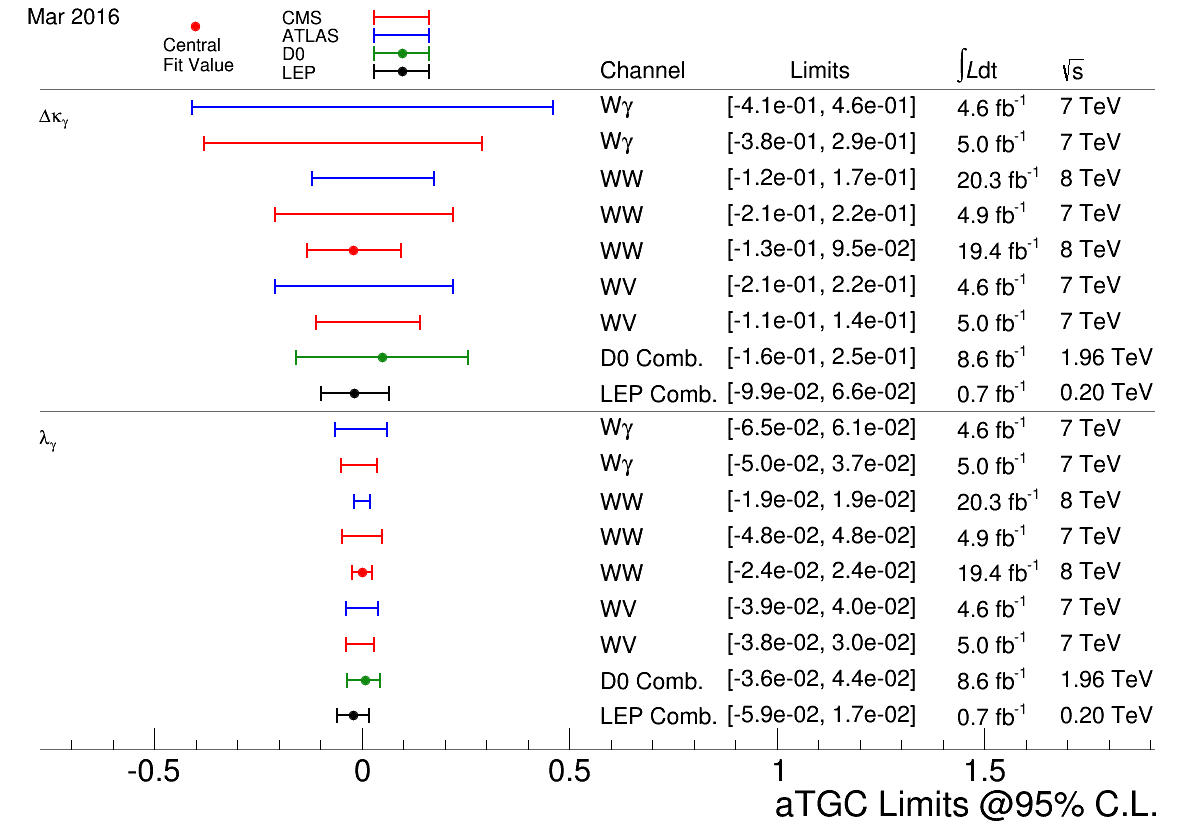
\includegraphics[width=0.80\textwidth]{../figs/WgAbout/aTGC_cg.png}}
    \caption{Summary of limits on the $WW\gamma$ aTGC coupling constants. Figure from~\cite{ref_twiki_SMP_ATGC}.}
    \label{fig:aTGC_cg}
  \end{center}
\end{figure}

The most recent measurements of $W\gamma$ production were performed by CMS~\cite{ref_7TeV_CMS} and ATLAS~\cite{ref_7TeV_ATLAS} collaborations with $pp$ collisions at $\sqrt{s}=7$~GeV collected in~2011. Both collaborations considered two channels: $W\gamma\rightarrow\mu\nu\gamma$ and $W\gamma\rightarrow e\nu\gamma$.\\

%The measurements are based on~5~fb$^{-1}$ and~4.6~fb$^{-1}$ of integrated luminosity with CMS and ATLAS respectively.

Diboson processes are rare in $pp$-collisions and analysts have to filter out events of their interest from many processes which are more likely to happen. To do that, a variety of selection criteria are applied which reject most of the background events to increase the signal fraction in the selected sample as much as possible. However, even after all possible selection criteria are applied, the majority of selected events are still background events and it is not possible to reduce the background any further without also significantly reducing signal.\\

The major source of such irreducible background is the fake photon background where hadronic jets are misidentified as photons. Such events originate mostly from $W+$jets, but $Z+$jets and $\bar{t}t+$jets events contribute to this source of background as well. In the electron channel there is one more significant background that is the fake photon background where electron is misidentified as a photon.  Such events are coming from $Z+$jets events. For the muon channels this background is small. Other sources of backgrounds for both channels include real-$\gamma$, fake lepton + real photon and fake lepton + fake photon backgrounds. The major source of real-$\gamma$ background is the $Z\gamma$ process where a final state lepton and a photon mimics the $W\gamma$ final state. Fake lepton + real photon background originates from the $\gamma+$jets process where a jet is misidentified as a lepton. Fake lepton + fake photon backgrounds come from dijet and multijet events where one of the jets is misidentified as a lepton and the other one is misidentified as a photon. The probability of a jet to be misidentified as a lepton is very small, therefore fake lepton + real photon and fake lepton + fake photon backgrounds are negligible.\\

Both channels provide measurements of $P_T^\gamma$ spectra because this variable is the most sensitive to the potential aTGC. The $P_T^\gamma$ spectra of the selected events in data superimposed with selected events in the simulation of the signal and estimated background contribution for the muon and electron channels are shown in Fig.~\ref{fig:Wg7TeV_CMS_ptGamma} for CMS and in Fig.~\ref{fig:Wg7TeV_ATLAS_ptGamma} for ATLAS measurement. Both measurements show a good agreement between data and the simulation.\\

%To derive aTGC limits...

\begin{figure}[htb]
  \begin{center}
    {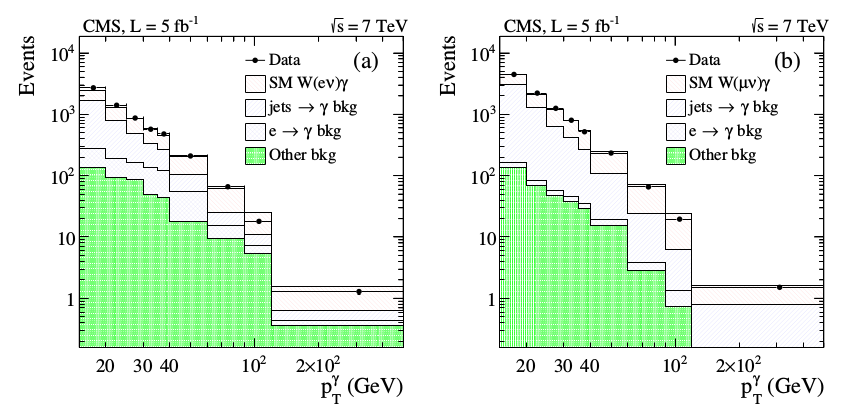
\includegraphics[width=0.80\textwidth]{../figs/WgAbout/Wg7TeV_CMS_ptGamma.png}}
    \caption{The distribution of the $p_T^\gamma$ of W$\gamma$ candidates in the analysis of~7~TeV CMS data. Data vs signal MC + background estimates. Left: $W\gamma\rightarrow e\nu\gamma$, right: $W\gamma\rightarrow \mu\nu\gamma$~\cite{ref_7TeV_CMS}.}
    \label{fig:Wg7TeV_CMS_ptGamma}
  \end{center}
\end{figure}

\begin{figure}[htb]
  \begin{center}
    {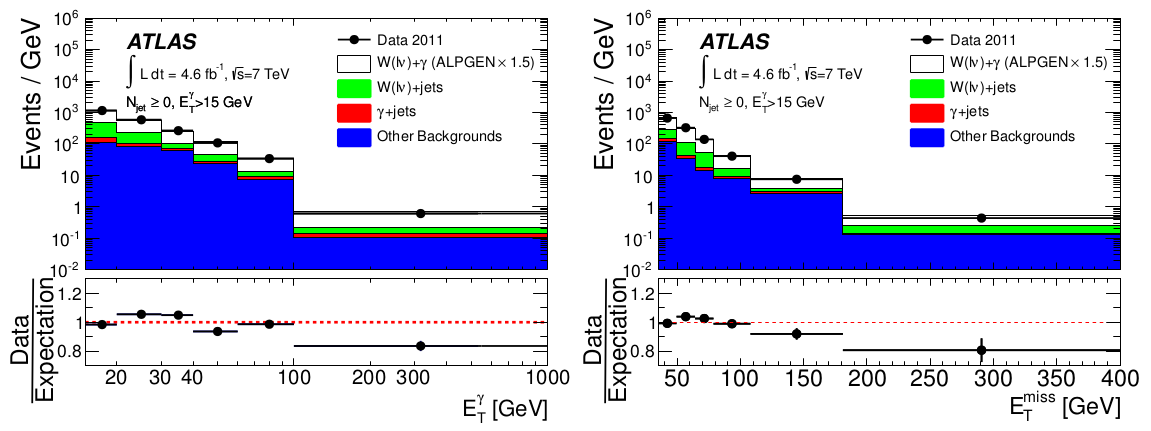
\includegraphics[width=0.80\textwidth]{../figs/WgAbout/Wg7TeV_ATLAS_ptGamma.png}}
    \caption{The distribution of the photon transverse momentum (left) and missing transverse momentum (right) of W$\gamma$ candidates in the analysis of 7 TeV ATLAS data. Data vs signal MC + background estimates~\cite{ref_7TeV_ATLAS}. }
    \label{fig:Wg7TeV_ATLAS_ptGamma}
  \end{center}
\end{figure}

The phase space restrictions of $W\gamma$ measurements come from the considerations of the detector acceptance, reducing heavily background-dominated regions and theoretical considerations such as to avoid divergence of the cross section and to reduce ISR and FSR contributions to the cross section.\\

CMS provides measurements of the $P_T^\gamma$ spectrum, the total cross section within the phase spaces of $\Delta R>0.7$, $P_T^\gamma>15$~GeV, $P_T^\gamma>60$~GeV and $P_T^\gamma>90$~GeV.\\

ATLAS, in addition to the $P_T^\gamma$ spectrum, total cross section and limits, provides the differential cross section and cross section with different number of associated jets. The phase space restrictions for ATLAS measurement include requirements on charged lepton kinematics $P_T^l>25$~GeV, $|\eta_l|<2.47$, requirements on the transverse momentum of a neutrino $P_T^\nu>35$~GeV, photon kinematics $P_T^\gamma>15$~GeV, $|\eta^\gamma|<2.37$, photon isolation fraction $\epsilon^P_h<0.5$ and lepton-photon separation $\Delta R(l,\gamma)>0.7$. For the differential cross section in number of associated jets, the requirements on jets kinematics and jets separation from leptons and photons are also applied: $E_T^{jet}>30$~GeV, $|\eta^{jet}|<4.4$, $\Delta R(e/\mu/\gamma,jet)>0.3$. No evidence of new physics is observed.\\

The estimated cross sections with any number of associated jets for $P_T^\gamma>15$~GeV are \\

\begin{equation}
\sigma(pp\rightarrow W\gamma\rightarrow l\nu\gamma) = 37.0 \pm 0.8\text{~(stat.)~}\pm 4.0\text{~(syst.)~}\pm 0.8\text{~(lumi.)~pb}
\end{equation}

\noindent{and} \\

\begin{equation}
\sigma(pp\rightarrow W\gamma\rightarrow l\nu\gamma) = 2.77 \pm 0.03\text{~(stat.)~}\pm 0.33\text{~(syst.)~}\pm 0.14\text{~(lumi.)~pb}
\end{equation}

\noindent{for CMS and ATLAS respectively. The results agree with NLO MCFM predictions of $31.81 \pm 1.8$~pb for the phase space used by CMS and of $1.96 \pm 0.17$~pb for the phase space used by ATLAS.}\\

In addition to the cross sections, both CMS and ATLAS provide limits on aTGC coupling constants $\Delta \kappa_\gamma$ and $\lambda_\gamma$. To do that, samples with non-zero aTGC coupling constants are generated, run through the whole reconstruction and selection procedures, and compared to the measured results of $P_T^\gamma$ spectra. The results on one-dimensional limits are quoted in Fig.~\ref{fig:aTGC_cg} while the results on two-dimensional limits can be found in~\cite{ref_7TeV_ATLAS},~\cite{ref_7TeV_CMS}.\\

In this dissertation we are measuring total and differential $d\sigma/d P_T^\gamma$ cross section. While the aTGC limits are not derived in this dissertation, the measured differential cross section can be used to derive them. The measurement details and results are described in Chapter~\ref{sec:AN_WgMeas}.\\


\section{Experimental Setup} % 7-20 pages
\label{sec:Exp}
\section{Large Hadron Collider}
\label{sec:Exp_LHC}
% brochure: http://cds.cern.ch/record/1165534/files/CERN-Brochure-2009-003-Eng.pdf
% brochure, page 12-13 (16-17 of pdf doc)

The LHC~\cite{ref_LHC_brochure,ref_LHC_TDR,ref_LHC_website} is the largest particle accelerator and the most ambitious particle physics research facility ever built. The LHC accelerates two particle beams up to near the speed of light. The beams travel in opposite directions, each in its own beam pipe, in ultrahigh vacuum. The beam is made up of protons which are grouped as bunches separated by several meters from each other. Each bunch contains~$10^{11}$~protons. The bunches of protons are accelerated by varying electromagnetic fields, focused by superconducting quadrupole magnets and steered by dipole magnets. The bunches collide at fixed collision points where particle detectors are placed. Particles are produced in the collisions and registered by the detectors to be subsequently used to accomplish physics goals of the experiments.  

%Beams are prepared, shaped, focused
%Beams travel in vacuum in beampipes
%Beam structure is bunches (define what they are)
%Bunches are accelerated by varying EM field in RF cavities
%Bunches are focused by focusing superconducting quadrupole magnets
%Bunches are steered by dipole magnets

The LHC is located in the tunnel at the France-Switzerland border. The tunnel is located as deep as~175~meters underground, its circumference is about~27~km.

Before entering LHC, particle beams go through several stages of acceleration, and the LHC is the final machine of the chain of the CERN's accelerator complex (Fig.~\ref{fig:CERN_accelerator_complex}). Protons are extracted from hydrogen atoms, are accelerated by Linac2 to energies of~5~MeV, and are then injected into the Proton Synchrotron Booster (PSB) where they reach energies of~1.4~GeV. After that, protons are sent to PS and then to Super PS (SPS) where they are accelerated up to~25~GeV and~450~GeV respectively. Finally, protons enter the LHC and are accelerated to reach their collision energies of several TeV per beam. Besides protons, the complex also accelerates and collides lead ions. However, in this dissertation we analyze data from $pp$ collisions only.   

\begin{figure}[htb]
  \begin{center}
    {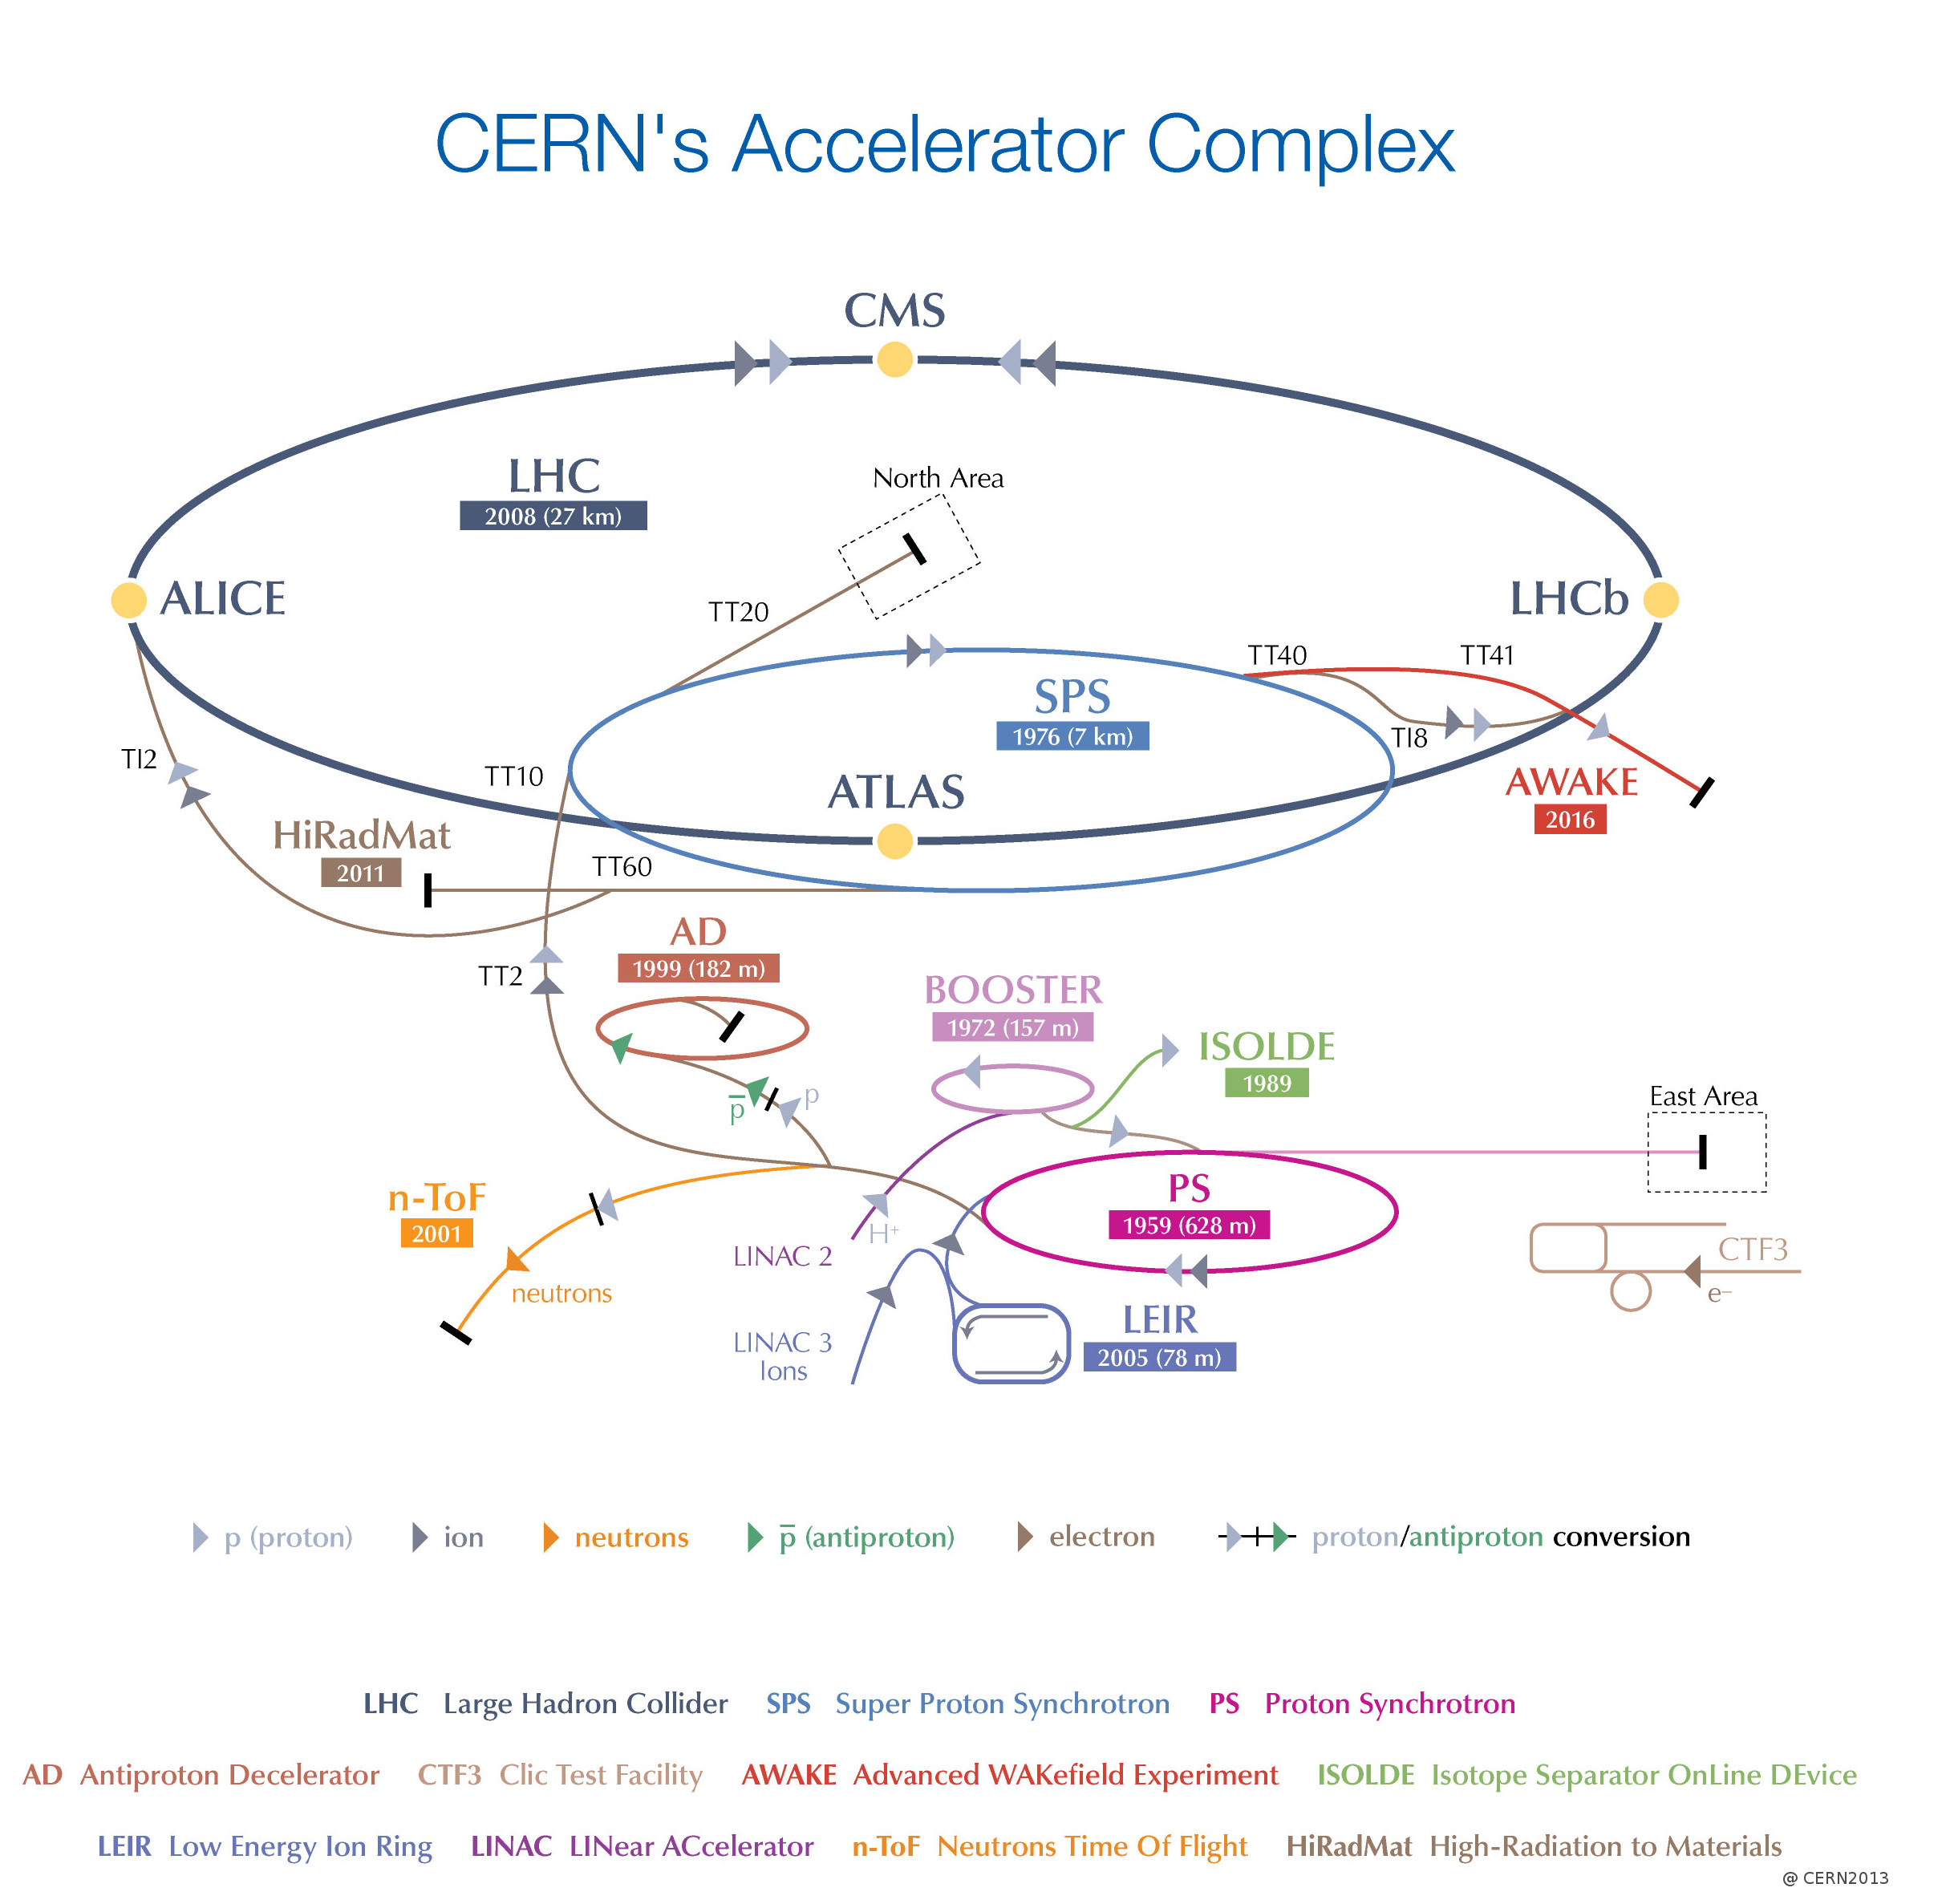
\includegraphics[width=0.98\textwidth]{../figs/Exp/CERN_accelerator_complex2013.jpg}}
    \caption{CERN's accelerator complex~\cite{ref_fig_CERNacceleratorComplex}.}
    \label{fig:CERN_accelerator_complex}
  \end{center}
\end{figure}

% brochure, page 15-17 - skip (19 of pdf doc)
% PLACE this sentence somewhere else; the rest of material is too basic

%brochure, page 18 (20 of pdf doc)

%brochure p 38 (42 of pdf doc) 
%Main goals of LHC were to detect the SM Higgs boson if it existed and to search for evidences of BSM physics which may give a clue on understanding the phenomena including but not limited to the dark matter, the matter-antimatter asymmetry, the nature of the gravitational force. 

Six detectors are installed at the LHC to detect products of hadron collisions and to perform the measurements of the LHC physics program. ATLAS and CMS are general purpose detectors designed to explore a broad spectrum of particle physics questions within and beyond the SM, LHCb specializes in the physics of B mesons, ALICE is designed to detect products of heavy ion collisions, LHCf and TOTEM are small detectors with very specialized research goals. LHCf and TOTEM are installed close to the ATLAS and CMS collision points respectively and are referred as forward detectors. 

%The greatest achievement by the LHC today is the discovery of the Higgs boson in~2012 by the CMS~\cite{ref_HiggsPaperCMS} and the ATLAS~\cite{ref_HiggsPaperATLAS} collaborations. 

%brochure 27 (31 of pdf doc)

%LHC is constructed of eight arcs, each arc corresponds to a sector as shown in Fig.~\ref{fig:LHCsectors}. In between there are eight insertions where beams are either collided or injected or dumped or cleaned. On the other hand, LHC is split on eight octants, each starting from the middle of one sector and ending at the middle of the next one. Thus, each octant includes one full insertion.\\ 

The design collision energy of the LHC is $\sqrt{s}=$14~TeV which corresponds to~7~TeV per beam. However, several lower energy points were probed. In~2010-2011 the LHC operated at an energy of~3.5~TeV per beam which was already higher than the energy of any other collider. In~2012 the beam energy was increased up to~4~TeV. In~2013-2014 the LHC was shut down for upgrades. Collisions were restarted at~6.5~TeV in~2015 and continued at this energy in~2016. At any energy point, both LHC beams have equal energies.

All critical measurements performed at lower energies are also repeated at higher energies. For the BSM searches, the ability to probe higher energy scales increases our chances for a discovery. For a SM cross section measurement, it needs to be done at all energies and compared to the theory since cross sections evolve with energy (Fig.~\ref{fig:LHC_totalCS}). While cross sections of parton-parton collisions typically decrease with energy, $pp$ or $\bar{p}p$ cross sections increase because as we go higher in $\sqrt{s}$, more partons in a given protons have enough energy to produce a certain type of interaction. This enables the observation of rarer processes as we increase energy. 

\begin{figure}
  \centering
  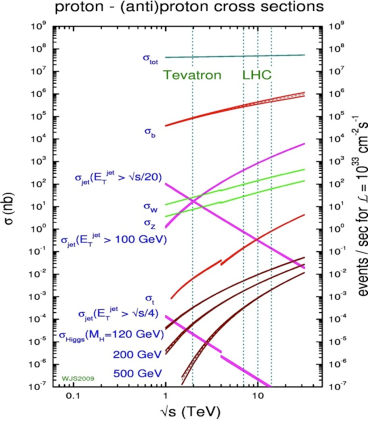
\includegraphics[width=.65\linewidth]{../figs/Exp/LHC_totalCS.png}
  \caption{Cross sections of different processes in $pp$ and $\bar{p}p$ collisions~\cite{ref_fig_LHC_totalCS}.}
  \label{fig:LHC_totalCS}
\end{figure}

%\begin{figure}
%  \centering
%  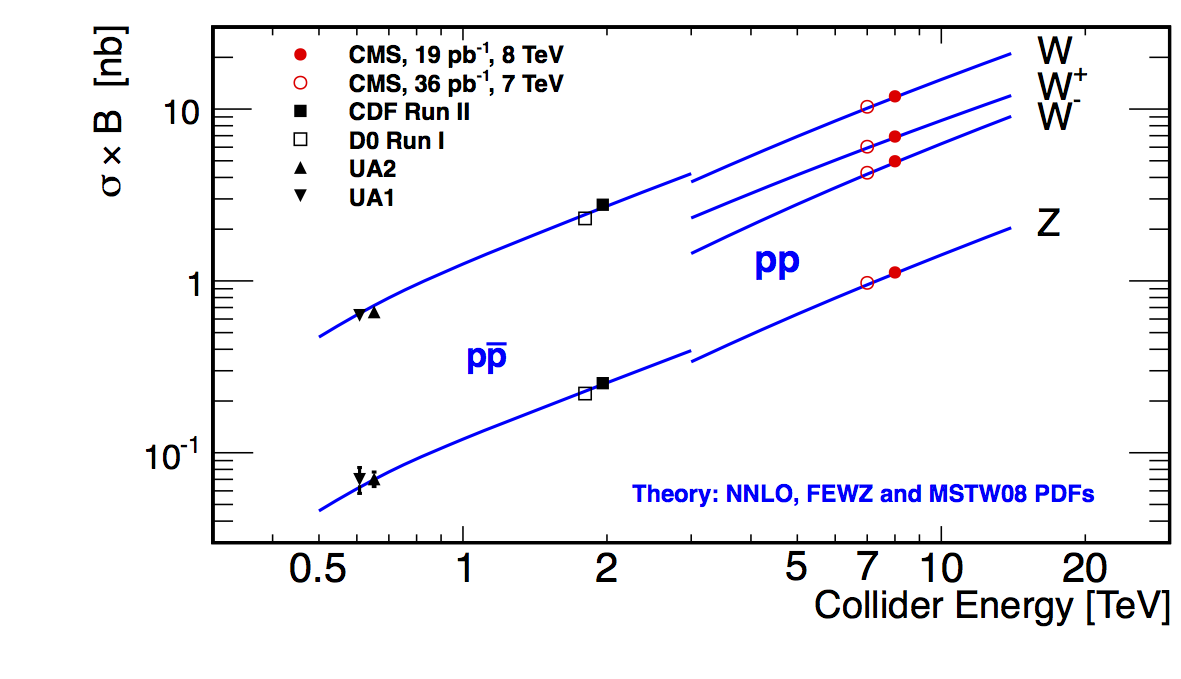
\includegraphics[width=.80\linewidth]{../figs/Exp/cms-sigma-vs-e.png}
%  \caption{Cross section of $W$ and $Z$ production in $pp$ collisions~\cite{ref_fig_LHC_CS_WandZ}.}
%  \label{fig:LHC_CS_WandZ}
%\end{figure}

%While different BSM searches have been constituting a significant part of the LHC physics program since the beginning of its operation, no deviations from the SM were found by any of the experiments. The searches continue with higher beam energies and larger amount of data.

In addition to the beam energy, there are many other collider parameters which reflect the ability of the collider to achieve stated goals. A brief summary of them is available in Tab.~\ref{tab:LHCparameters}. One of the most critical parameters of an accelerator is the luminosity which determines how many interesting events can be produced (Ch.~\ref{sec:WgAbout_LumiAndCS}). The instantaneous luminosity is determined by the following expression~\cite{ref_PDG}:

\begin{equation}
L^{inst} = f \frac{n_1 n_2}{4 \pi \sigma_x \sigma_y}
\end{equation}

\noindent{where $n_1$ and $n_2$ are numbers of particles in colliding bunches, $f$ is a frequency of collisions, $\sigma_x$ and $\sigma_y$ characterize sizes of overlapping parts of colliding beams in horizontal and vertical directions. The instantaneous luminosity multiplied by a cross section of a process gives an event rate (Eq.~\ref{eq:L_eventRate}) of this specific process. If we know the instantaneous luminosity and the theoretically predicted cross section of the process, we can estimate how many events per unit time of this particular process will be produced by our experiment. To estimate how many events of the process will be produced during a certain time period, we have to use the integrated luminosity which is an integral of the instantaneous luminosity over time:}

\begin{equation}\label{eq:integratedL}
  L = \int L^{inst} dt
\end{equation}

\noindent{The integrated luminosity of a data sample is a measure of the size of the data sample.}

The integrated luminosity of the LHC for $pp$ collisions for different years of the operation is shown in Fig.~\ref{fig:LHClumi}. Run~I of the LHC operation covers run periods of~2010-2012. While running at the energy of $\sqrt{s}=7$~TeV, LHC delivered~$L=$45~pb$^{-1}$ and~$L=$6.1~fb$^{-1}$ of data in~2010 and~2011 year respectively. In~2012 the working energy of LHC was $\sqrt{s}=$8~TeV, and the integrated luminosity was $L_{int}=$23.3~fb$^{-1}$.  After a long shutdown, LHC was upgraded for Run~II, to operate at $\sqrt{s}=$13~TeV in~2015 and delivered~$L_{int}=$4.2~fb$^{-1}$ of data by the end of~2015. In~2016 LHC continued operating at $\sqrt{s}=$13~TeV and delivered the integrated luminosity of~$L_{int}=$41.1~fb$^{-1}$~\cite{ref_LHClumi_twiki}.

The measurement of this dissertation is performed at the energy of~4~TeV per beam or the center of mass energy $\sqrt{s}=$8~TeV with~19.6~fb$^{-1}$ of data collected in~2012. The same process was measured at $\sqrt{s}=$7~TeV with about four times less data by both CMS and ATLAS. These measurements are discussed in greater detail in Ch.~\ref{sec:WgAbout_PastMeas}.

% brochure page 30 (34 of pdf)
\begin{table}[h]
  \begin{center}
  \caption{ Main parameters of LHC~\cite{ref_LHC_brochure}}
  \vspace{5 mm}
  \begin{tabular}{|l|c|}
     \hline
     Circumference & 27 km  \\ \hline
     Dipole operating temperature &  1.9 K \\ \hline
     Number of magnets &  9593 \\ \hline
     Number of main dipoles &  1232 \\ \hline
     Number of main quadrupoles &  392 \\ \hline
     Number of RF cavities &  8 per beam \\ \hline
     Nominal energy, protons &  7 TeV \\ \hline
     Nominal energy, lead ions &  2.76 TeV per nucleon \\ \hline
     Peak magnetic dipole field &  8.33 T \\ \hline
     Min. distance between bunches &  7 m \\ \hline
     Design luminosity &  $10^{34}$ cm$^{-2}$ s$^{-1}$ \\ \hline
     No. of bunches per proton beam &  2808 \\ \hline
     No. of protons per bunch (at start) &  $1.1\times 10{11}$ \\ \hline
     No. of collisions per second &  600 millions \\ \hline
  \end{tabular}
  \label{tab:LHCparameters}
  \end{center}
\end{table}

\begin{figure}
  \centering
  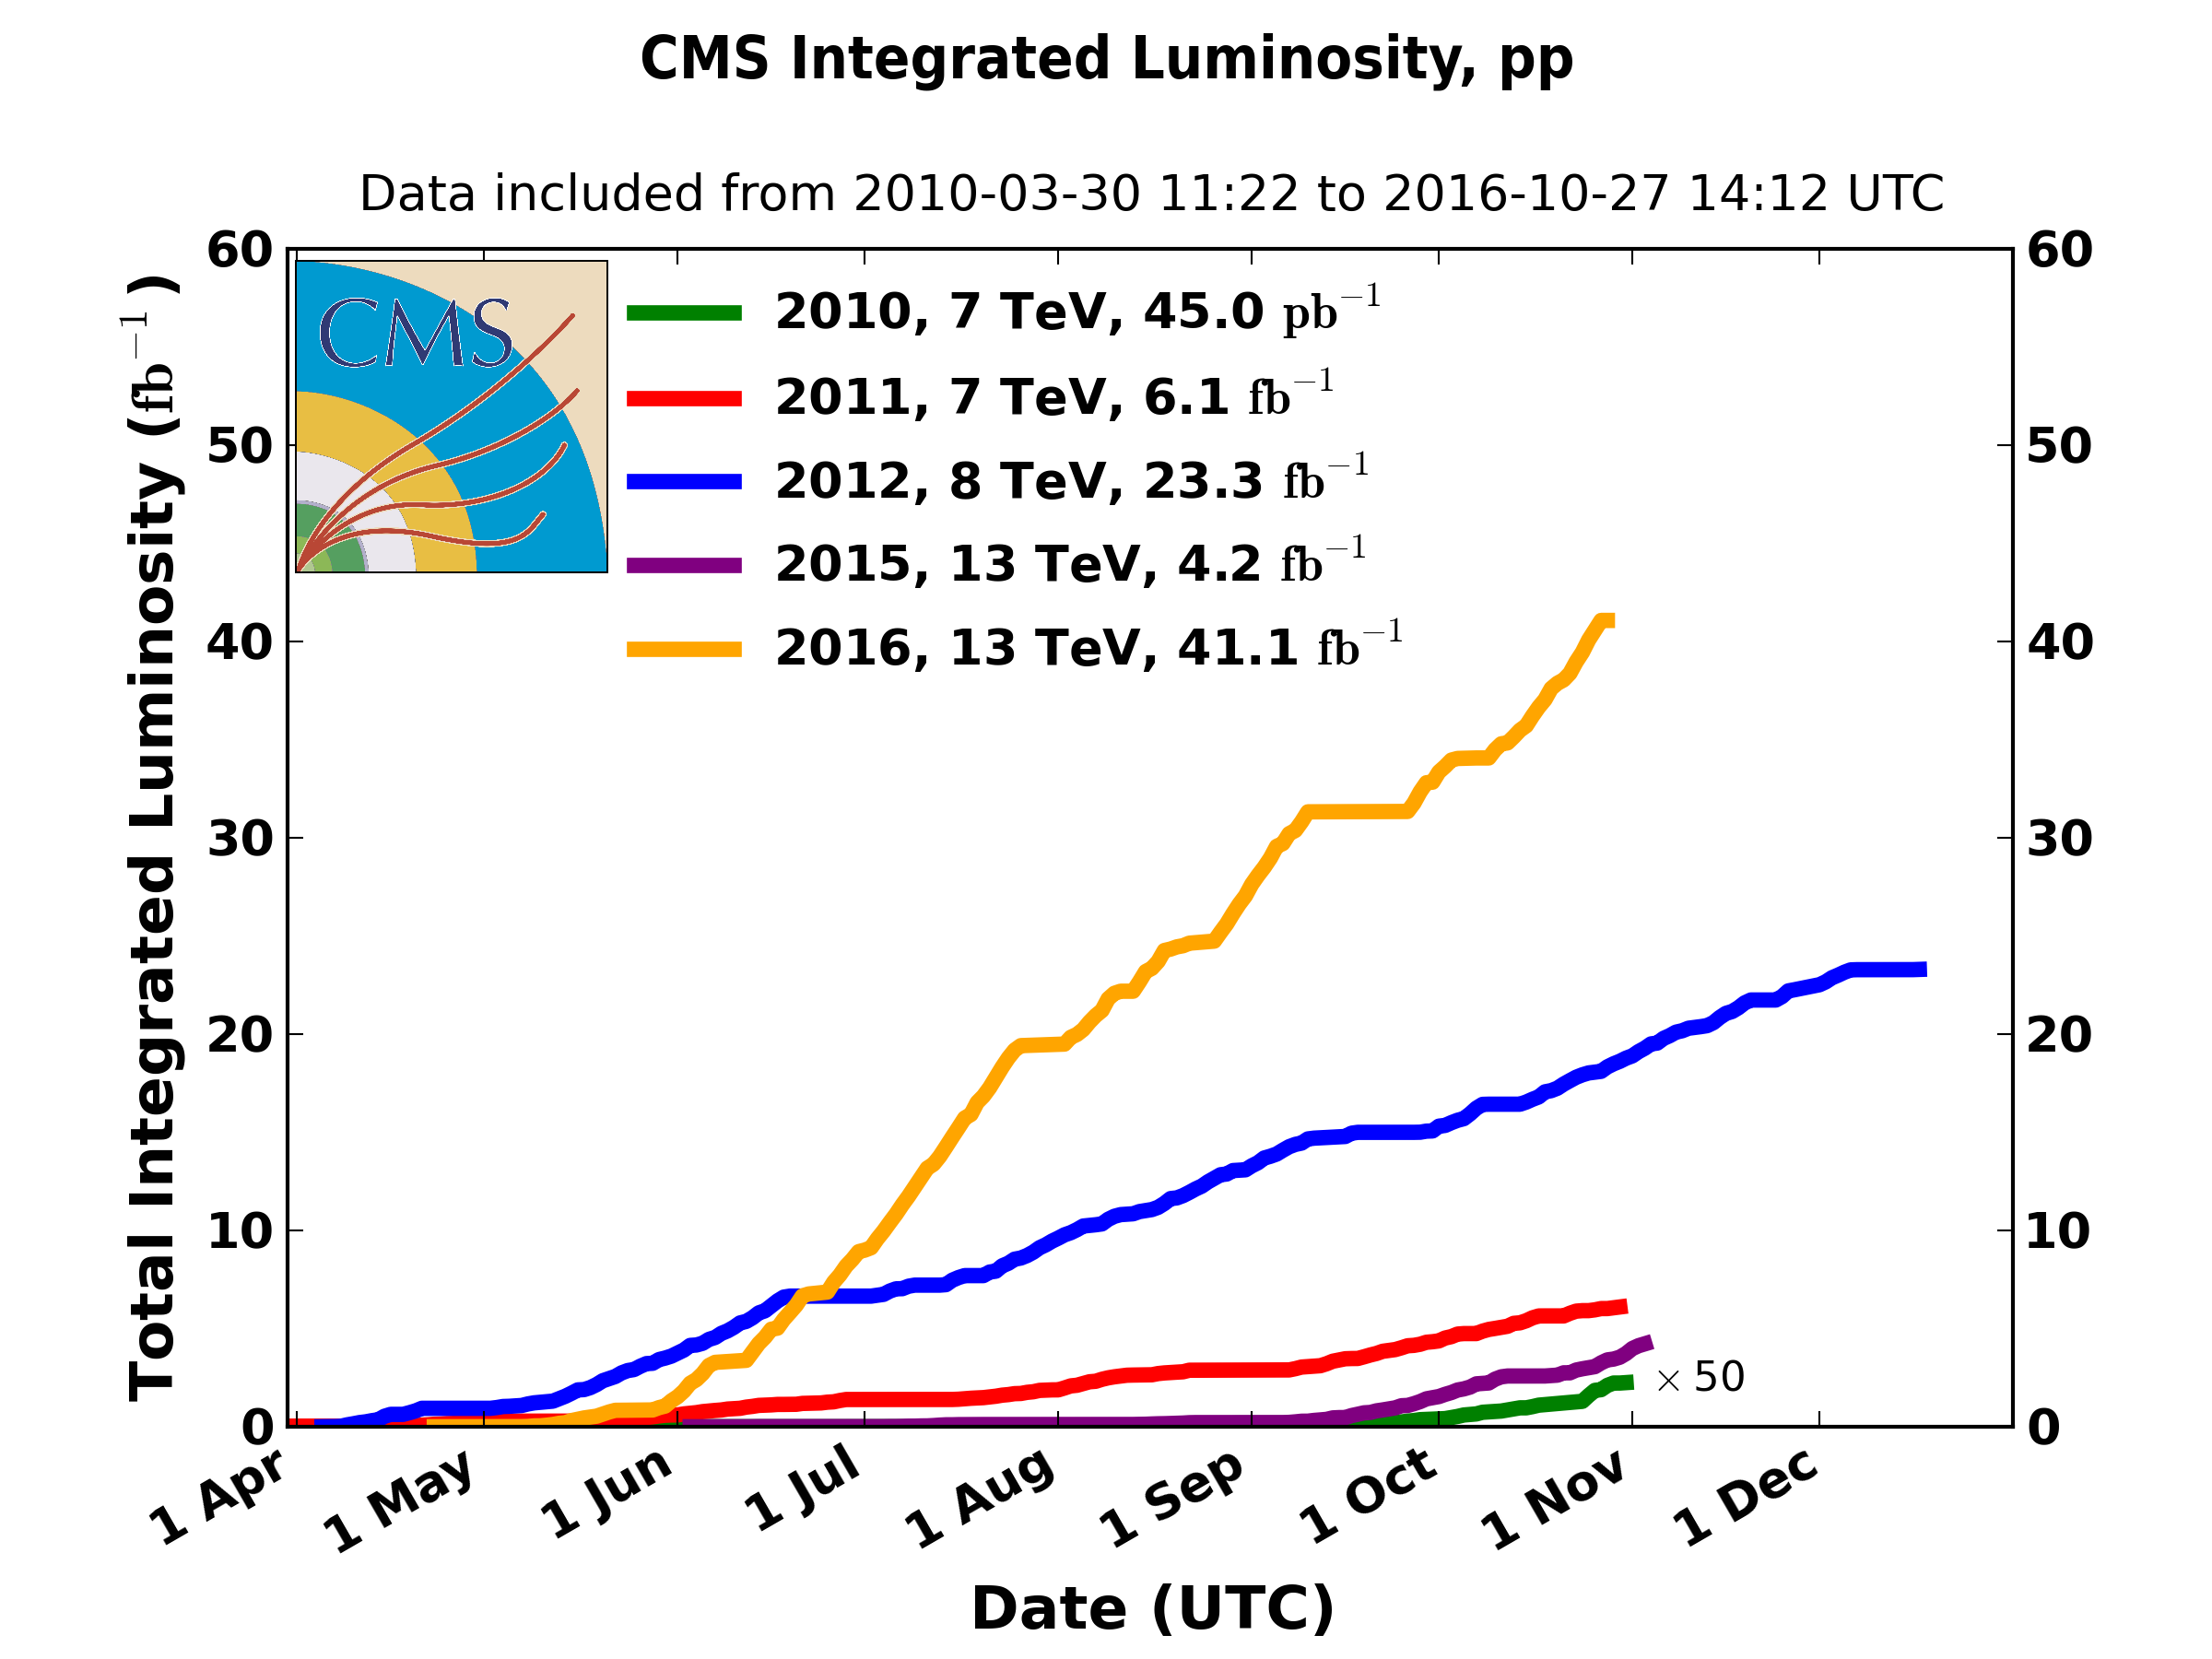
\includegraphics[width=.80\linewidth]{../figs/Exp/int_lumi_cumulative_pp_2.png}
  \caption{LHC integrated luminosity by year~\cite{ref_fig_LHClumi}.}
  \label{fig:LHClumi}
\end{figure}

% begin: LHC lumi and LHC sectors
%\begin{figure}
%\centering
%\begin{minipage}{.48\textwidth}
%  \centering
%  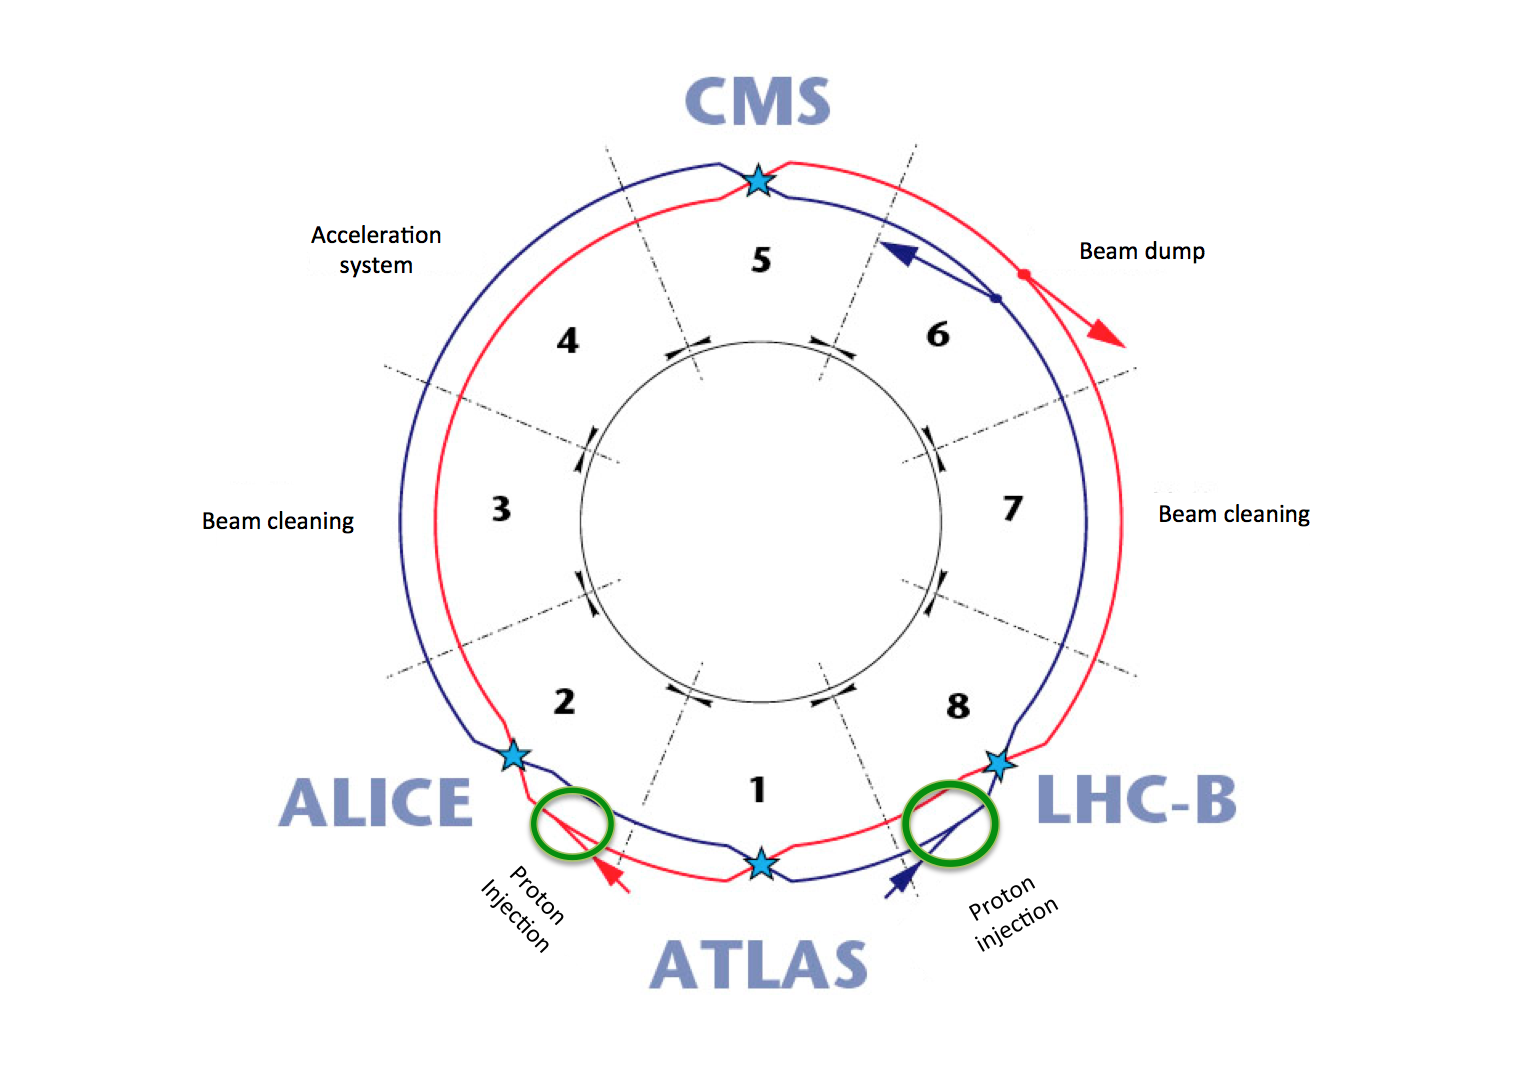
\includegraphics[width=.95\linewidth]{../figs/Exp/LHC_sectors.png}
%  \caption{Schematic view of LHC sectors. Source of the figure: \cite{ref_fig_LHCsectors}.}
%  \label{fig:LHCsectors}
%\end{minipage}%
%\begin{minipage}{.48\textwidth}
%  \centering
%  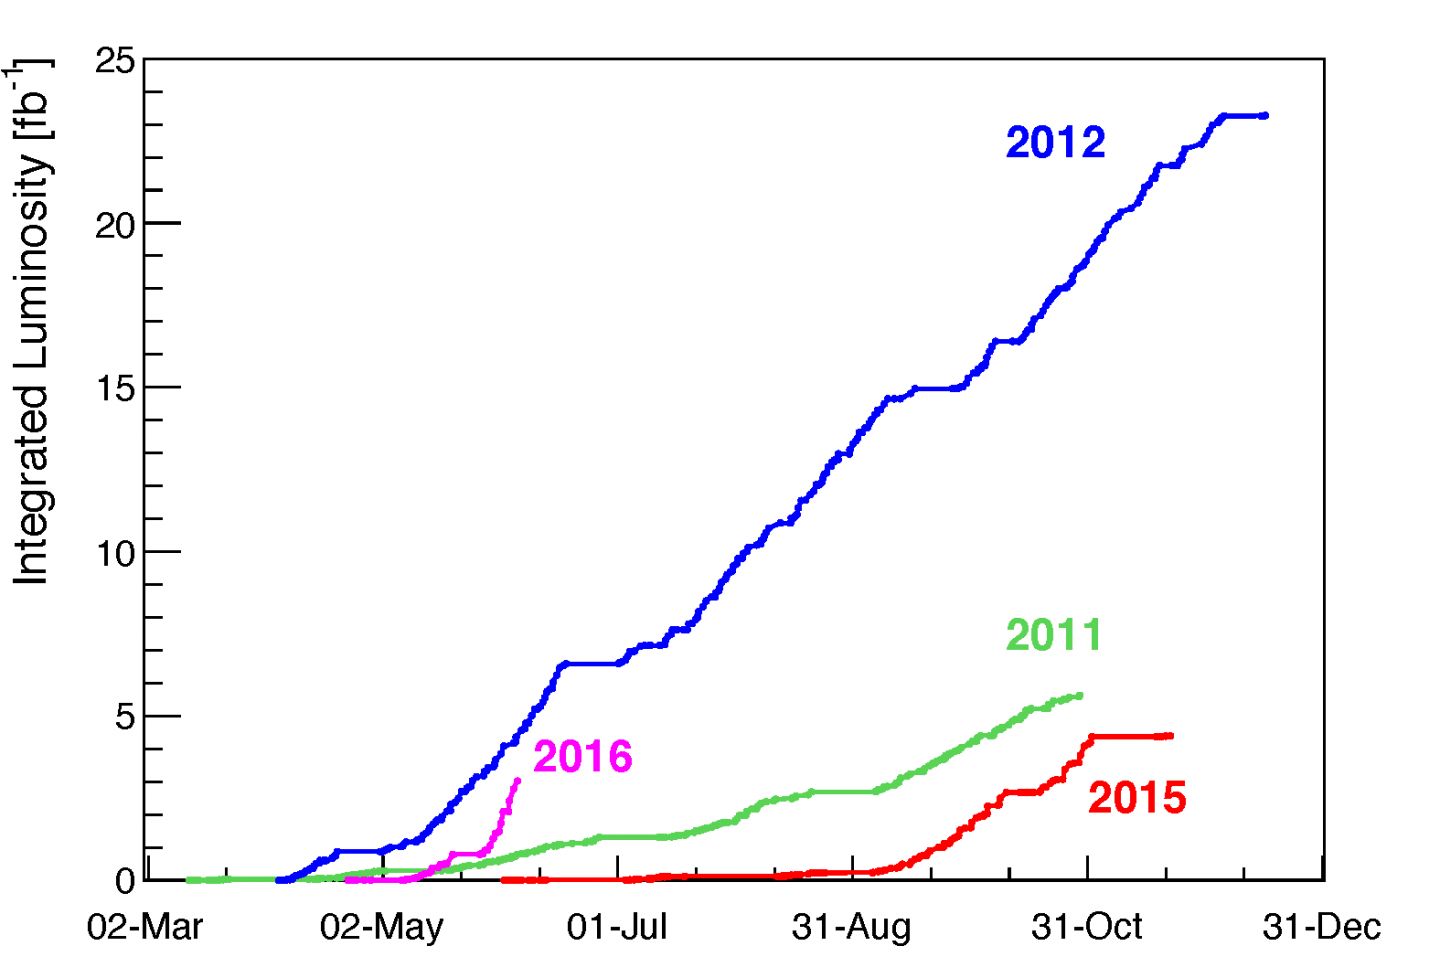
\includegraphics[width=.95\linewidth]{../figs/Exp/LHC_lumi.png}
%  \caption{LHC integrated luminosity by year. Source of the figure: \cite{ref_fig_LHClumi}.}
%  \label{fig:LHClumi}
%\end{minipage}
%\end{figure}
% end: LHC lumi and LHC sectors

\subsection{Compact Muon Solenoid}
\label{sec:Exp_CMS}
\subsubsection{Introduction}

CMS is a general-purpose detector designed for detecting various particles which are being produced in pp collisions at LHC. Its main feature is a huge magnet to create a magnetic field of 4T to curve charged particles in the tracking system and 2T outside to curve muons in the muon system.\\

CMS detector is a cylindrically symmetric with a colliding beam as a central axis. The detector consists, from inner to outer layer,  of a tracking system, an electromagnetic calorimeter (ECal), a hadronic calorimeter (HCal), a magnet and a muon system. Having the tracking system, ECal and HCal inside of a large solenoid makes the detector "compact". A segment of a CMS slice in $r-\phi$ plane is shown in Fig.~\ref{fig:CMS_slice}.\\

When a heavy particle is produced in a collision, it decays immediately, and we detect its long-living decay products including an electron, a photon, a muon, a neutral hadron or a charged hadron. Depending on the trace left by a particle in different subdetectors we can identify a particle. Electrons and positrons leave curved tracks in the tracking system and then induce showers in the electromagnetic calorimeter (ECal) where they are typically stopped. Photons induce the same electromagnetic showers is ECal however, as neutral particles, they do not leave tracks in the tracking system. Hadrons normally travel through the ECal undisturbed and induce a hadronic shower in the hadronic calorimeter (HCal). Charged and neutral hadrons can be distinguished from each other by checking whether they leave a track in the tracking system or not. Muons are the only particles which are not stopped by the layer of ferrum and leave tracks in the CMS muon system. Neutrinos are not detected by CMS. \\  

\begin{figure}[htb]
  \begin{center}
    {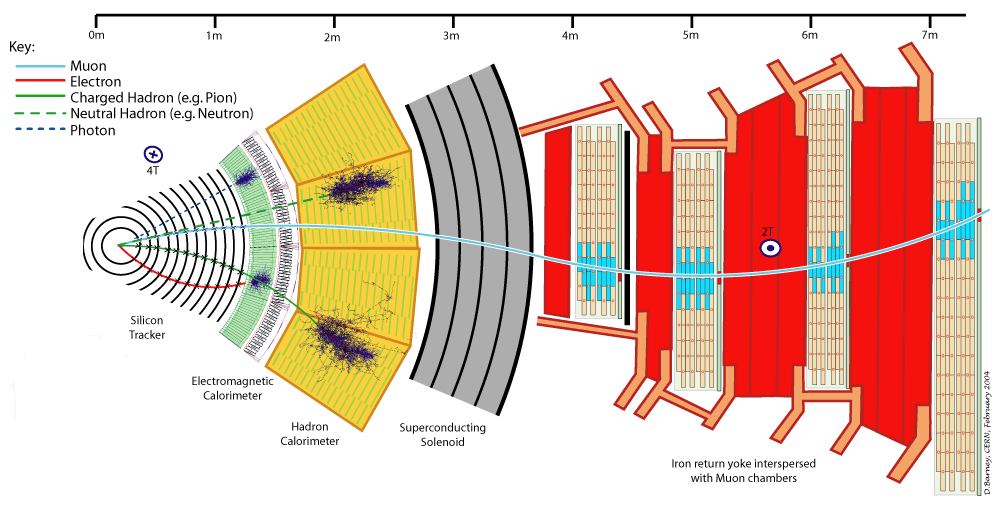
\includegraphics[width=0.98\textwidth]{../figs/Exp/CMS_Slice.png}}
    \caption{CMS slice.}
    \label{fig:CMS_slice}
  \end{center}
\end{figure}

% CMS detector geometry and variables

% In this dissertation...
In $W\gamma$ measurement we have muons and electrons as final state particles. They are both affected by CMS magnetic field allowing the tracking system and the muon system to measure their trajectory parameters and momenta.\\
In this dissertation we use the information of the primary vertex determined by the tracking system to select our events. Also the tracker provide us the information about electrons trajectories and momenta in the electron channel and distinguishes between electrons and photons.\\

\subsubsection{Magnet}

A magnetic field in a particle detector is necessary to measure momenta of charged particles by track curvatures. The higher the momentum is, the less a particles's path is affected by the magnetic field. In CMS it is done in the tracking system for all charged particles and in the muon system for muons.\\

The CMS magnet is placed between layers of HCal and a muon system. It creates a magnetic field of 4T inside the magnet, for the tracking system, and 2T outside the magnet, for the muon system. It is necessary to have stronger field in the tracking system because a density of tracks is much higher there than in the muon system and also the tracking system is much smaller and, therefore, more significant cuvature is necessary to measure the momentum with high precision.\\

The magnet is made of superconducting wires. An electric current flowing in the wires creates a uniform field inside the solenoid and also provides a magnetic filed of a certain configuration outside the solenoid.\\

\subsubsection{Tracking System}

The tracking system measures track geometry including particles trajectories and locations of primary and secondary vertices and momenta of charged particles. It needs to disturb particles as little as possible so that they can pass through. Therefore, just a few measurements must be enough to reconstruct the track. The accuracy of a measurement of each hit is 10~$\mu$m.\\

The tracking system consists of silicon pixels and silicon strips (Fig.~\ref{fig:tracker_slice}). Collision tracks start at the center and then cross the layers of the tracking system. Tracks are straight in $r-z$ plane and curved by the magnetic field in the $r-\phi$ plane. The acceptance of the tracker system in $r-z$ plane is geometrically limited by $\eta=2.5$ ($\eta=-\ln[ {\tan{\theta/2}}]$, where $\theta$ is a polar angle).\\

The pixel tracker is the closest subsystem of CMS to the collision point thus it receives the largest particle flux: at~8~cm from the collision point the flux is about~10~million $1/(cm^2 s)$, and the pixel detector with its~65~millions sensors is capable to reconsruct all these tracks. It consists of three layers of cylinders in the barrel with radii of~4~cm,~7~cm and~11~cm and four disks in the endcap, two disks at each side. The tracker is designed in such a way that a single track hits multiple sensors. Then the trajectory is reconstructed based on how much charge is collected on each sensor. This allows us to reach a spacial resolution of 15-20~$\mu$m which is much smaller than a distance between sensors.\\

The strip tracker is placed right after the pixel tracker and occupies the detector volume up to~130~cm aound the beam axis. The strip tracker consists of four parts: the tracker inner barrel (TIB), the tracker inner disks (TID), the tracker outer barrel (TOB) and the tracker endcap (TEC) as shown in Fig.~\ref{fig:tracker_slice}. In the strip tracker there are over 15,000 sensitive modules with a total number of~10~million strips. Each sensitive module consists of a set of sensors, its support structure and readout elements.\\

%electric charge and amplification

%limitations

\begin{figure}[htb]
  \begin{center}
    {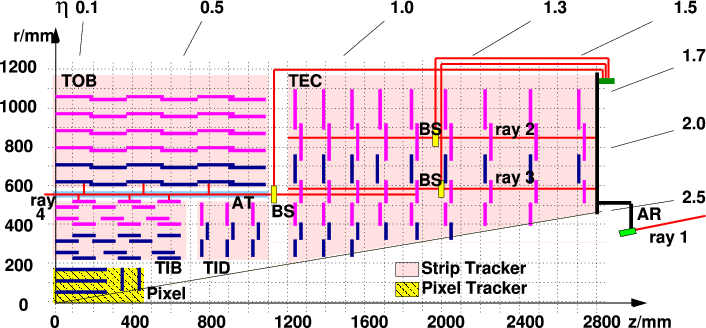
\includegraphics[width=0.8\textwidth]{../figs/Exp/tracker_slice.png}}
    \caption{Slice of the CMS tracking system in $r-z$ plane.}
    \label{fig:tracker_slice}
  \end{center}
\end{figure}

\subsubsection{Electromagnetic Calorimeter}

The ECal measures energy of electrons and photons and also measures geometries of their trajectories. Electrons and photons interact with the ECal substance by inducing electromagnetic showers. Traces left by photons and electrons in the ECal are the same. To distinguish between these two particles, it is necessary to perform matching to the track in the tracking system. If there is a track, then there is an electron (or positron). If there is no track, then the particle is a photon.\\

The Ecal is a layer between the tracking system and the HCal. It is made of high-density lead tungstate crystals arranged in a barrel section and two endcap sections. The crystals work as scintillators. When electrons and photons pass through it, it produces light proportional to the particle's energy. The scintillated light then is amplified by photomultipliers producing signals on sensitive elements.\\

It is important for the Ecal to be able to distinguish between high energetic photons and pairs of lower energetic photons e.g. from a $\pi^0$ decay. It is especially difficult in the endcap sections where angle between two photon trajectories is small. Ecal preshowers located in front of the endcaps which have much smaller granularity provide extra spacial precision. Their strips are~2~mm wide compared to~3~cm wide crystals in the main volume of the ECal.\\

%(Why muons and hadrons don't release their energy here?)
%limitations

\subsubsection{Hadron Calorimeter}

The HCal is placed right after the ECal and is the last subdetector within the magnet. The HCal measures energies of charged and neutral hadrons. In addition, the HCal determines the track parameters. Match to the tracking system has to be done: if a matching track found, then it is a chagred hadron otherwise it is a neutral hadron. \\
%(Why muons don't release their energy here? Would photons and electrons release the energy here?)

The HCal consists of alternate layers of absorbers and scintillators. Hadrons hit brass or steel plate of absorber producing secondary particles. When emerge into the scintillator, the particles induce hadronic and electromagnetic showers and emit blue-violet light which is further shifted to the green region and read out by special boxes within the HCal. The secondary hadrons produced during the interaction with the absorber interact with the next absorber producing more showers in the next layers of scintillators and also affect the total enegry deposit. All hadrons must be stopped inside the layers of the HCal.\\

%HCal Sampling calorimeter (?)
%Hybrid Photodiodes

\subsubsection{Muon System}

Muons pass through the ECal, the HCal and the magnet without interacting. They are the only particles which are registered in the muon system which is placed outside the magnet and which is the largest part of CMS detector.\\

There are four concentric layers of muon detectors (stations) and iron return yoke between them. Muons induce several hits in the muon stations which are later fitted and matched to the tracking system measurements to provide the best possible resolution in the measurements of all parameters of the muon's trajectory and momentum.\\

Overall, there are 1400 muon chambers including 250 drift tubes (DTs), 540 cathode strip chambers (CSCs) and 610 resistive plate chambers (RPCs).\\

The system of DTs measures positions of muons in the barrel. Each DT chamber is about~2~m by~2.5~m in size. It consists of~12~layers of aluminium which are groups by four. There are up to~60~drift tubes in a layer. The middle group of layers measures $z$-coordinate and two other groups determine the perpendicular coordinate.\\

Each drift tube is~4~cm in width, is filled with a gas and has a wire inside. When a charged particle passes through the volume, it ionizes atoms and the wire receives an electric charge.\\

% (how it works? why do we need it?)

% Copypaste: In total there are 1400 muon chambers: 250 drift tubes (DTs) and 540 cathode strip chambers (CSCs) track the particles’ positions and provide a trigger, while 610 resistive plate chambers (RPCs) form a redundant trigger system, which quickly decides to keep the acquired muon data or not. 

cathode strip chambers
resistive plate chambers

\begin{figure}[htb]
  \begin{center}
    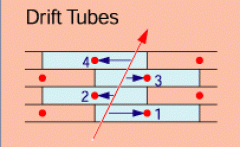
\includegraphics[height=2.5 cm]{../figs/Exp/muonSystem_driftTubes.png}\quad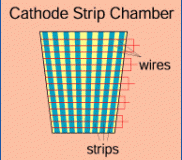
\includegraphics[height=2.5 cm]{../figs/Exp/muonSystem_CSC.png}\quad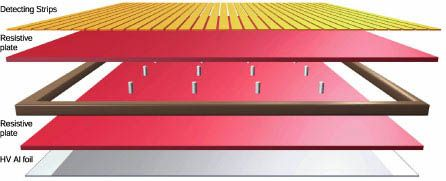
\includegraphics[height=2.5 cm]{../figs/Exp/muonSystem_RPC.png}
    \caption{Components of the CMS muon system. Left to right: drift tubes, cathode strip chambers (CSCs), resistive plate chambers (RPCs).}
    \label{fig:muonSystem}
  \end{center}
\end{figure}


\subsubsection{Triggering and Data Aquisition}
Level-I trigger
High Level Trigger

\subsubsection{Event Reconstruction}
Where to place particle reconstruction, particle flow algorithm and MET? Check other theses

Acceptance: particles which are too collinear and go to pipe; particles which get curved too strongly


\section{CMS Tracker Alignment} % 5-10 pages
\label{sec:alignment}
\section{Approach}
\label{sec:alignmentAlg}
%(mostly along the lines of my presentation for the USCMS workshop because it was time when I was the most active)

%Why align?\\
%How to align?\\
%When align?\\
%How to check that your alignment is good?\\

% DOUBLE CHECK WITH FRANK'S PRESENTATION
% MAKE SURE THERE IS NO PLAGIARISM
The concept of track-based alignment can be illustrated in the example of the alignment of a toy tracker (Fig.~\ref{fig:toyTracker_part1}-\ref{fig:toyTracker_part2}). A charged particle crosses a toy tracker of six flat equidistant modules. Because real geometry of the tracker differs from the ideal one, hits are recorded at the places different from the design ideal places. We record and process a large number of tracks to determine positions and orientations of the modules.

\begin{figure}[htb]
    \begin{center}
        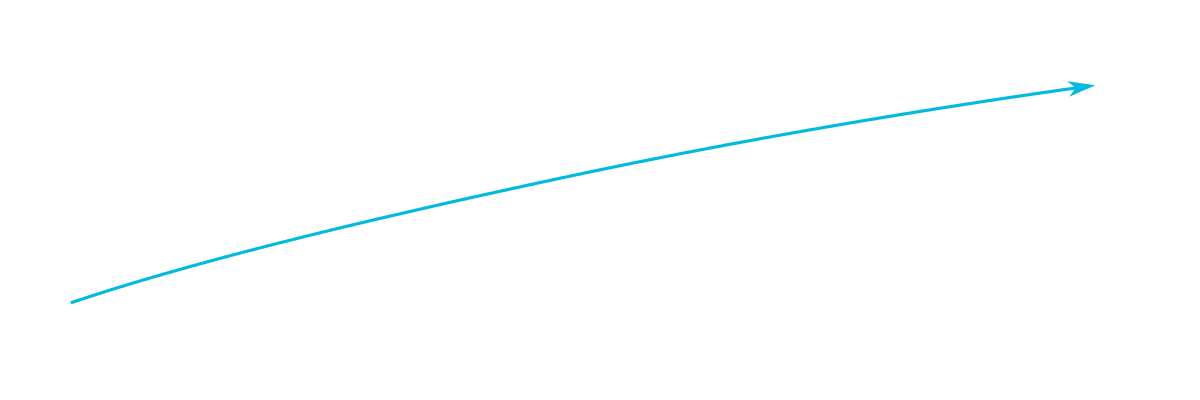
\includegraphics[width=0.45\textwidth]{../figs/Alignment/toyTracker01.png}
        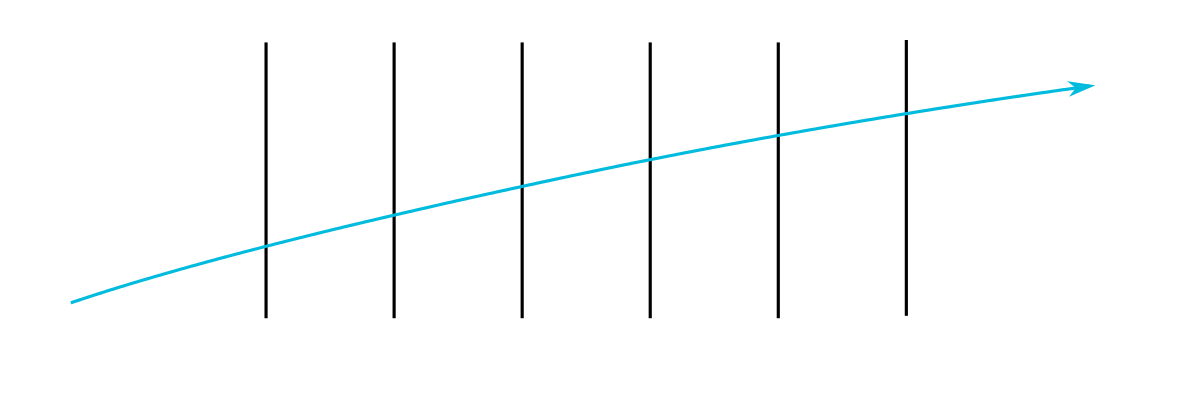
\includegraphics[width=0.45\textwidth]{../figs/Alignment/toyTracker02.png}
        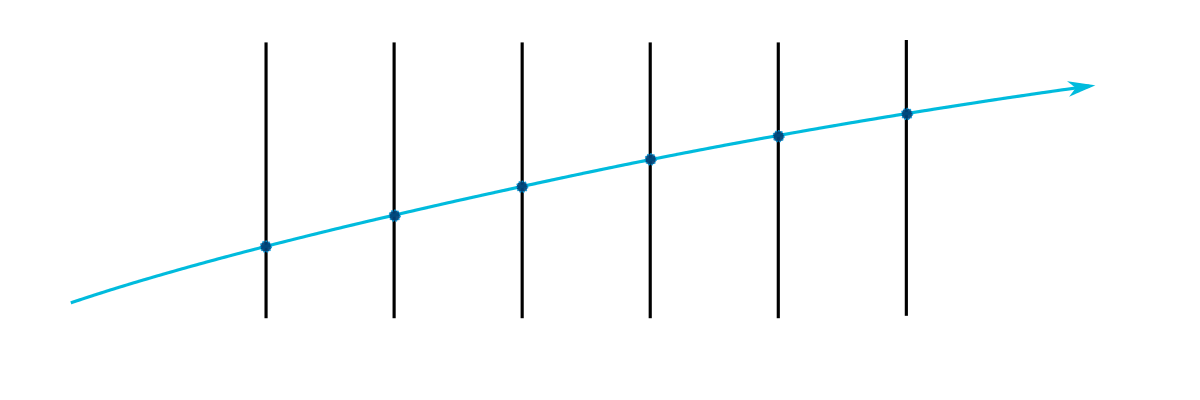
\includegraphics[width=0.45\textwidth]{../figs/Alignment/toyTracker03.png}
        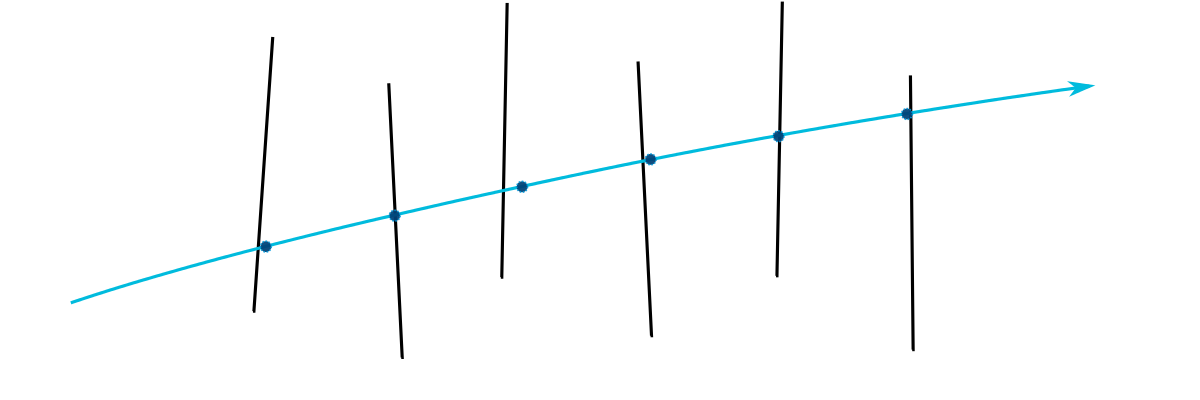
\includegraphics[width=0.45\textwidth]{../figs/Alignment/toyTracker04.png}
        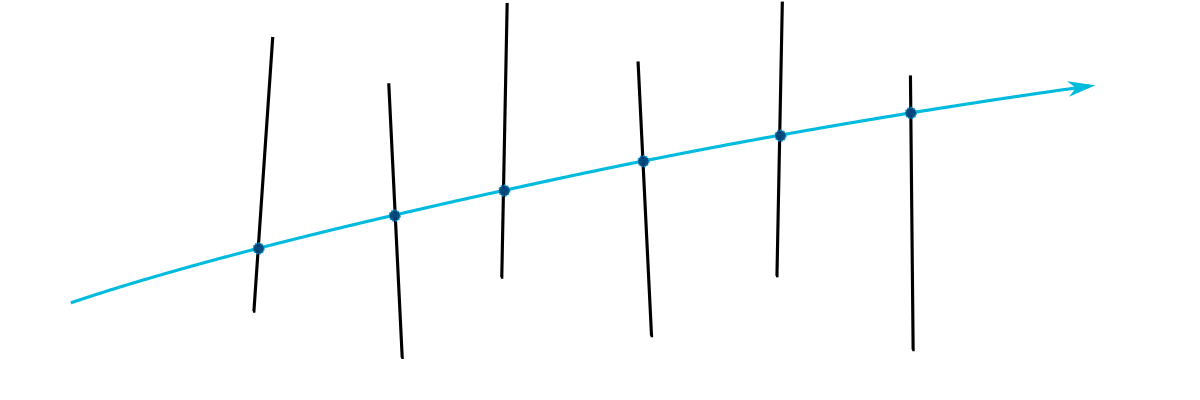
\includegraphics[width=0.45\textwidth]{../figs/Alignment/toyTracker05.png}
        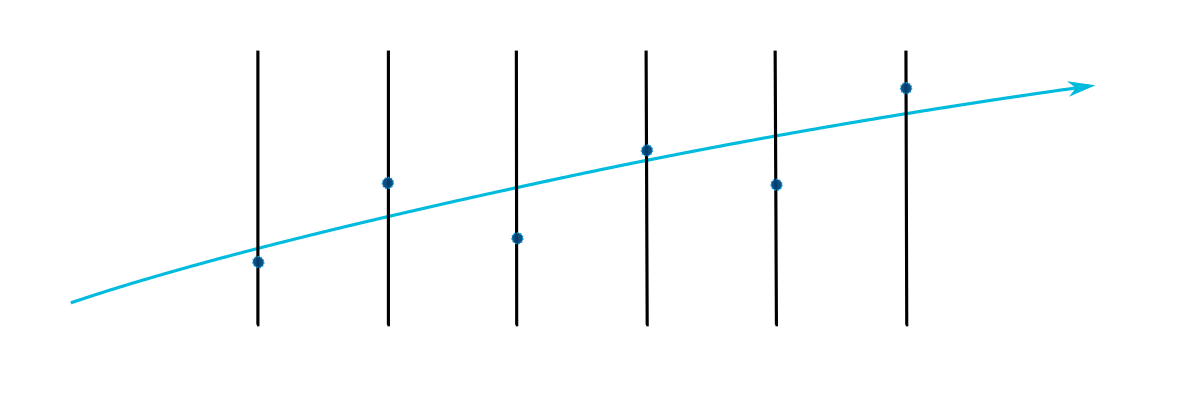
\includegraphics[width=0.45\textwidth]{../figs/Alignment/toyTracker06.png}
    \end{center}
    \caption{The alignment of a toy tracker, part. When a charged particle passing through a detector (top left), it crosses a toy tracker which consists of six flat equidistant modules (top right). If the modules were placed exactly at their designed positions, we would observe the hits exactly at the points where the track crosses modules of ideal geometry (middle left). However, in reality, the positions and tilts of the modules are different from ones suggested by the ideal geometry (middle right). Hits, indeed, are recorded at the places where modules are mounted, not at the design ideal places (bottom left). If we assumed a tracker to be ideal and a track to be smooth, we would see that our hits are off-track (bottom right). Image by Frank Meier.}
    \label{fig:toyTracker_part1}
\end{figure}

\begin{figure}[htb]
    \begin{center}
%        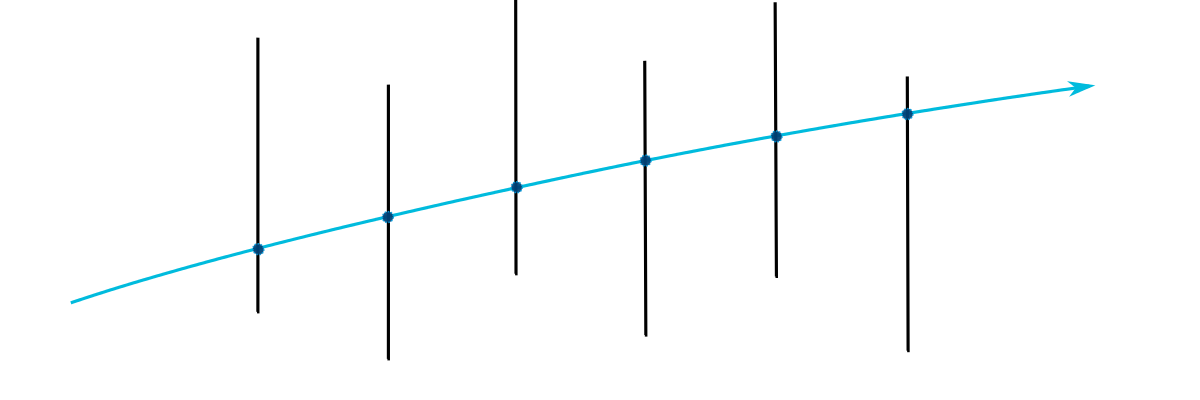
\includegraphics[width=0.45\textwidth]{../figs/Alignment/toyTracker07.png}
%        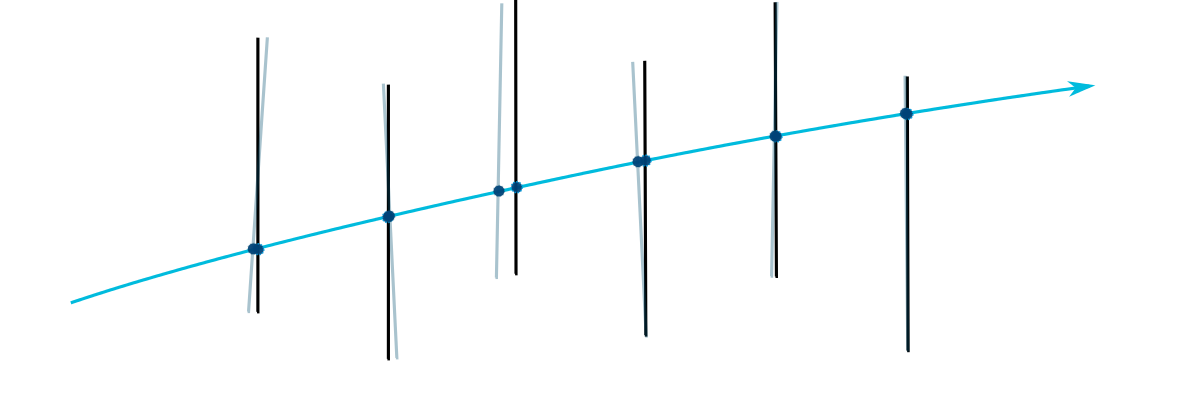
\includegraphics[width=0.45\textwidth]{../figs/Alignment/toyTracker08.png}
%        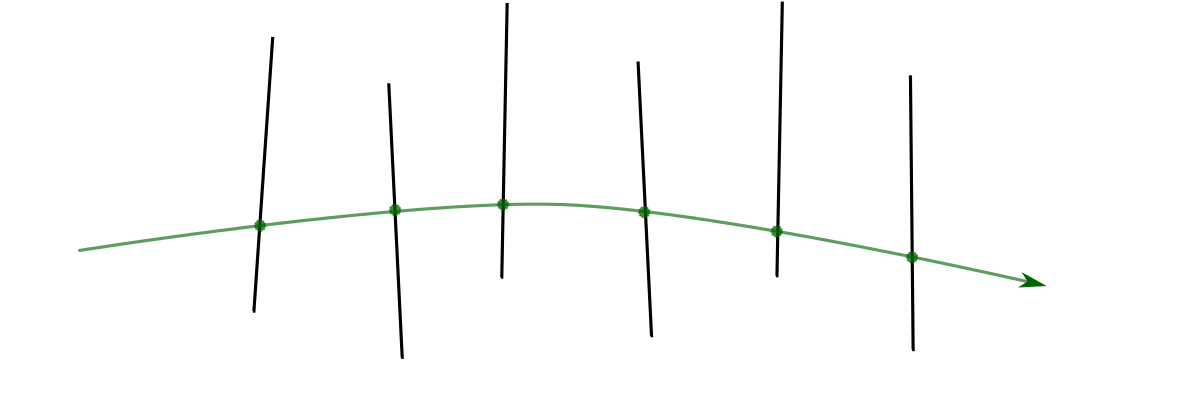
\includegraphics[width=0.45\textwidth]{../figs/Alignment/toyTracker09.png}
%        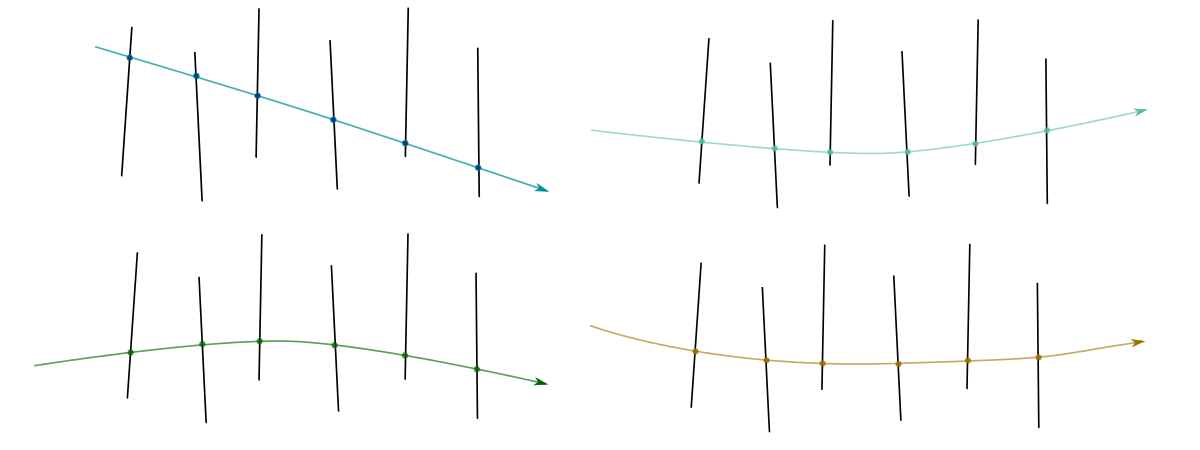
\includegraphics[width=0.45\textwidth]{../figs/Alignment/toyTracker10.png}
        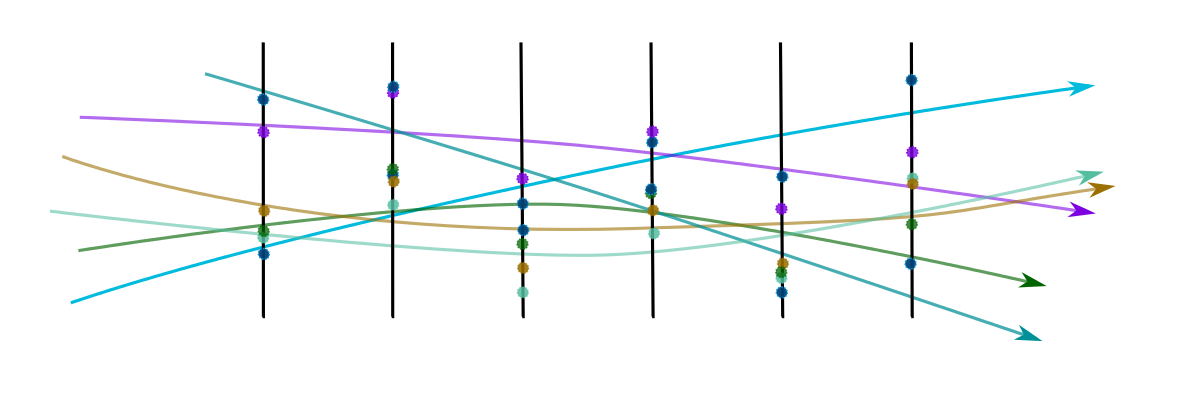
\includegraphics[width=0.45\textwidth]{../figs/Alignment/toyTracker12.png}
        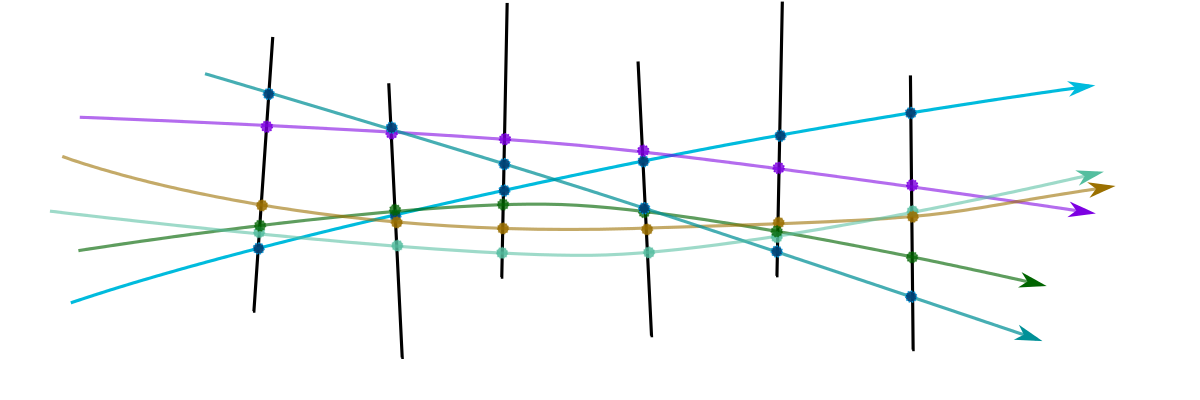
\includegraphics[width=0.45\textwidth]{../figs/Alignment/toyTracker13.png}
    \end{center}
    \caption{The alignment of a toy tracker, part~2. We record a large number of tracks and take into account them all to determine the alignment parameters by minimizing residuals between measured and predicted hits. Image by Frank Meier.}
    \label{fig:toyTracker_part2}
\end{figure}

%The CMS tracker contains 1440 silicon pixel modules in PXB and PXF and 15148 silicon strip modules in TIB, TOB, TID, TEC. 

The tracker alignment problem is a least squares problem. The expression to minimize is the following:

\begin{equation}
  \chi^2(\mathbf{p},\mathbf{q})=\sum_j^{tracks} \sum_i^{hits} \left( {\frac{m_{ij}-f_{ij}(\mathbf{p},\mathbf{q_j})}{\sigma_{ij}}} \right)^2,
\end{equation}

\noindent{where $\mathbf{p}$ are parameters describing the tracker geometry, $\mathbf{q}_j$ are parameters of the $j^{th}$ track, $m_{ij}-f_{ij}$ are distances between the measured hit and a position predicted by the track fit (``residuals''), $\sigma_{ij}$ is the Gaussian error of the measurement.} 

We can align the large substructures with respect to the global CMS coordinate system and individual modules with respect to the coordinate systems of their substructures. The parameters to align large substructures include three coordinates to determine location and three angles to determine orientation of the substracture. At the module level, we align positions and rotations with respect to the positions and angles of the corresponding large structure (Fig.~\ref{fig:alignmentParameters}). Also at the module level, we align for surface deformations which are described by three parameters per sensor (Fig.~\ref{fig:surfaceDeformations}). 

In addition to particles originating from $pp$ collisions of the LHC, CMS also detects muons that originate from interactions of cosmic particles with the Earth's atmosphere. Tracks left by these two types of particles in the tracking system are referred as collision and cosmic tracks respectively. We need both types of tracks for the alignment. %Cosmic tracks pass through the detector vertically and do not allow us to connect different subdetectors to one another. Collision tracks originate from the collision point and go in all directions. However, those tracks which cross TEC are all almost collinear and, therefore, it is difficult to measure $z$-coordinate of TEC modules with collision tracks only.

Two algorithms are used for the alignment of the CMS tracking system: Millepede-II~\cite{ref_MPII_Alg} and HIP~\cite{ref_HIP_Alg}. Millepede-II performs a simultaneous fit of all alignment parameters and all track parameters while HIP performs iterative fits of alignment parameters $\mathbf{p}$ and track parameters $\mathbf{q}_j$.

\begin{figure}[htb]
    \begin{center}
        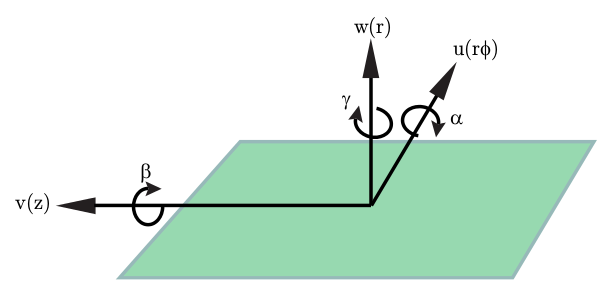
\includegraphics[width=0.70\textwidth]{../figs/Alignment/alignment_strip_coords.png}
    \end{center}
    \caption{Local alignment parameters~\cite{ref_Frank_thesis}.}
    \label{fig:alignmentParameters}
\end{figure}

\begin{figure}[htb]
    \begin{center}
        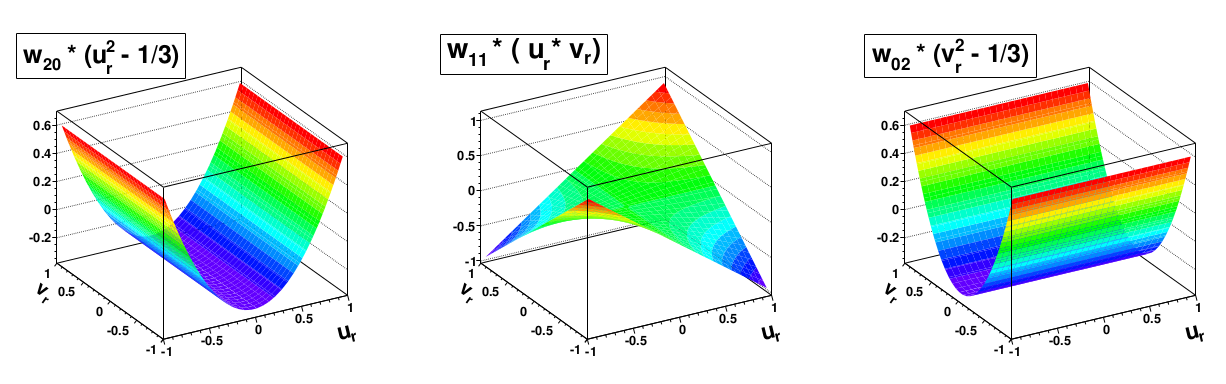
\includegraphics[width=0.90\textwidth]{../figs/Alignment/alignment_surface_deformations.png}
    \end{center}
    \caption{Surface deformations~\cite{ref_Alignment}.}
    \label{fig:surfaceDeformations}
\end{figure}

It is necessary to align a part of the tracking system whenever we suspect a physical change in a location or an orientation of this part. First of all, whenever a part of the CMS tracker is taken out and placed back, we need to realign it. Also whenever a magnet is turned on and off, different parts of the tracking system shift with respect to one another. Pixel half barrels are not screwed firmly, and are moving along each other on rails, therefore, they need to be aligned frequently. Realignment is also necessary when modules are replaced or when the temperature changes. %because it causes the module deformations. 

After the procedure of the tracking system alignment is performed, we validate the results. Chapter~\ref{sec:alignmentResults} discusses various tools of alignment validation using the example of the tracking system alignment based on the~2015 data.   

%\begin{figure}[htb]
%    \begin{center}
%        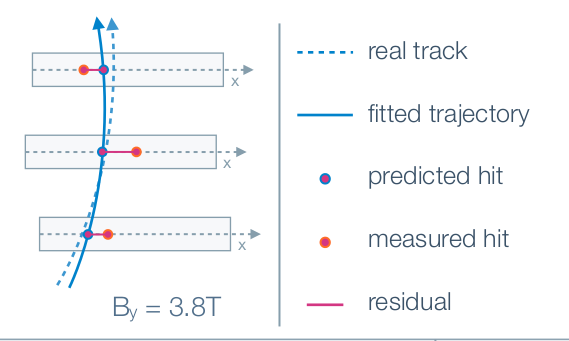
\includegraphics[width=0.70\textwidth]{../figs/Alignment/track.png}
%    \end{center}
%    \caption{Track residuals.}
%    \label{fig:trackAndResiduals}
%\end{figure}

%\begin{figure}[htb]
%  \begin{center}
%    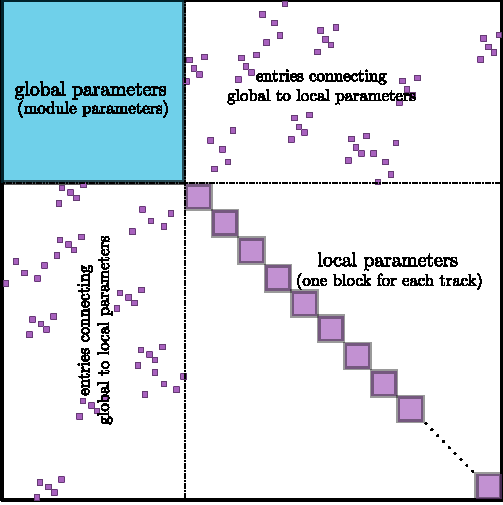
\includegraphics[width=0.70\textwidth]{../figs/Alignment/mpmatrix.pdf}
%  \end{center}
%  \caption{Track residuals.}
%  \label{fig:trackAndResiduals}
%\end{figure}

\section{Selected Results on Alignment of the Tracking System with~2015 Data}
\label{sec:alignmentResults}

Different data-taking periods in 2015 include periods of cosmic ray data-taking with the magnetic field $B=0$T and $B=3.8$T, and periods of collision data-taking at $\sqrt{s}=13$~TeV center-of-mass energy with $B=0$T and $B=3.8$T. Different data-taking periods correspond to different detector geometries particularly due to changes of the magnetic field. 

% (1) MY WORDS:
Alignment constants were derived separately for each of the data-taking periods using the alignment results of the previous period of data-taking as a starting point. Millepede-II and HIP algorithms were run in sequence to perform the alignment, as well as two algorithms, were run independently for cross checking. 

% (2) NO PLAGIARISM 
The first alignment of the tracker corrected for the displacements that took place between the Run~I and Run~II. Cosmic ray data with magnetic field turned on ($B=3.8$T) and off ($B=0$T) were used for this alignment. The modules in certain parts of BPIX were repaired during the shutdown, and all pixel subdetectors were moved within the tracker. 

After the cosmic ray data taking periods, the magnetic field was turned off again, and the first collisions were detected with $B=0$T. This change in the magnetic field caused movements in the tracking system that has the strongest effect in the pixel subdetectors. The alignment performed using~$B=0$T collisions and cosmic ray data recovers the tracker performance in the ability to reconstruct kinematic parameters of charged particles. When the magnetic field was turned back on, the large substructures of BPIX and FPIX have displaced again, and, thus, the tracking system was aligned again to recover these displacements.  

% (3) MY WORDS
Validation of tracking system alignment tools include geometry comparison tool (Ch.~\ref{sec:AlRes_GCP}), validation using distribution of median residuals (Ch.~\ref{sec:AlRes_DMRs}), cosmic track splitting validation (Ch.~\ref{sec:AlRes_trackSplit}), and primary vertex validation (Ch.~\ref{sec:AlRes_PVvalid}). Full results of the first alignment with Run~II data are available at~\cite{ref_AlApproved_twiki}.

\subsection{Geometry Comparison}
\label{sec:AlRes_GCP}

% (4) MY WORDS:
Geometry comparison visualizes differences in positions of modules between two different geometries of the CMS tracking system. Figure~\ref{fig:GCP_FPIX} shows the comparison between positions of the FPIX modules between Run~I and Run~II geometries. Each dot in the figure corresponds to one module. Four clusters of red dots (Fig.~\ref{fig:GCP_FPIX}, left) and shifted parts at ($\phi<-\pi/2$, $\phi>\pi/2$) and ($-\pi/2<\phi<\pi/2$) (Fig.~\ref{fig:GCP_FPIX}, right) represent displacements of four half-disks by~4.5 and~5.5~mm at the $-z$ side of the FPIX. At the $+z$ side of the FPIX small relative movements of individual modules are observed only. For more intuitive visualization, the three-dimensional plot of the pixel detector is produced (Fig.~\ref{fig:GCP_3D}).     

\begin{figure}[htb]
    \begin{center}
        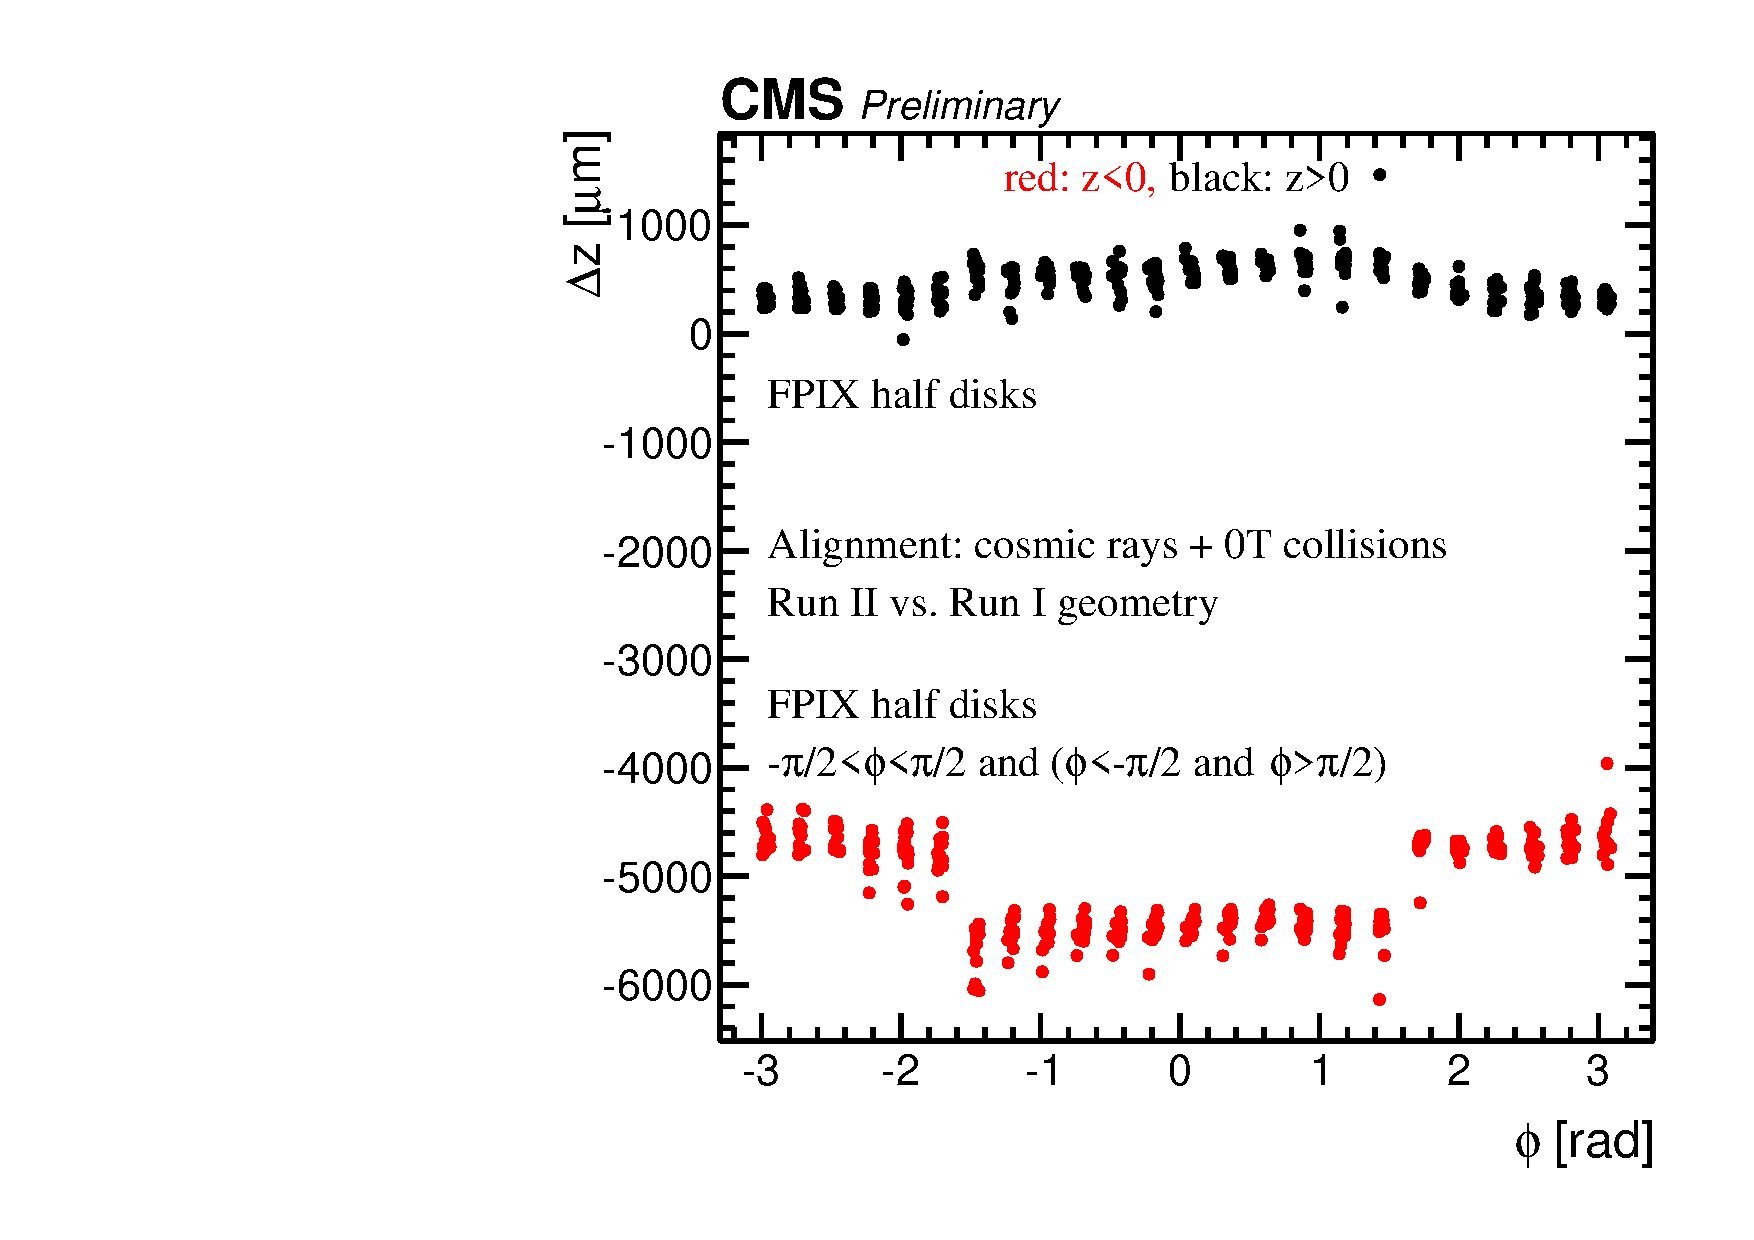
\includegraphics[width=0.45\textwidth]{../figs/Alignment/AlRes_phi_vs_dz_PXF_1.pdf}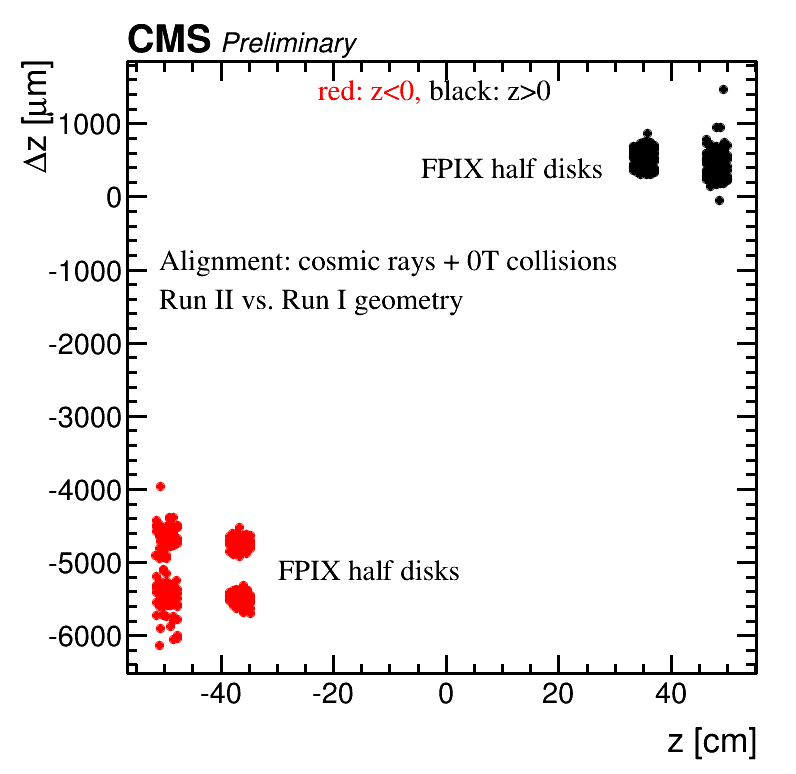
\includegraphics[width=0.45\textwidth]{../figs/Alignment/AlRes_z_vs_dz_PXF_1.png}
    \end{center}
    \caption{Comparison of Run~II and Run~I positions of the modules in the FPIX of the CMS tracking system. Positions are determined with the Millepede-II and HIP algorithms using cosmic ray data collected with the magnetic field of $B=0$T and $B=3.8$T magnetic field in the CMS solenoid. The difference $\Delta z$ (Run~II~-~Run~I) is plotted as a function of $z$ (left) and $\phi$ (right) in global coordinates.}
    \label{fig:GCP_FPIX}
\end{figure}

\begin{figure}[htb]
    \begin{center}
        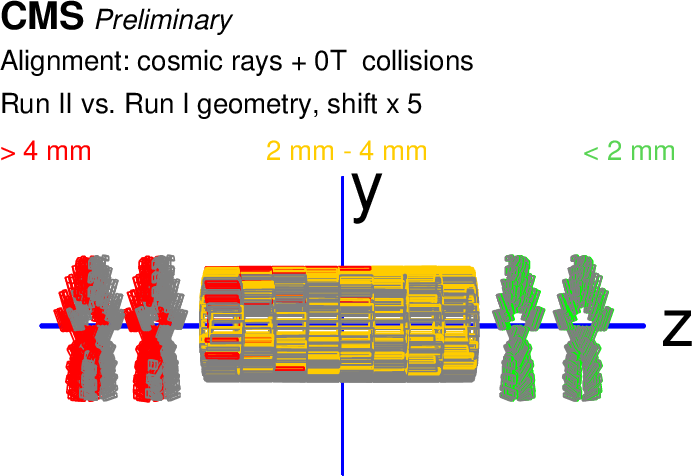
\includegraphics[width=0.95\textwidth]{../figs/Alignment/AlRes_RunIIvsRunI.png}
    \end{center}
    \caption{Three-dimensional geometry comparison of Run~II and Run~I positions in the BPIX and FPIX of the CMS tracking system. Positions are determined with the Millepede-II and HIP algorithms using cosmic ray data collected with the magnetic field of $B=0$T and $B=3.8$T magnetic field in the CMS solenoid and collision data with $B=0$T at $\sqrt{s}=13$~TeV. The positions at the end of Run~I are shown in gray. The module displacements between Run~I and Run~II are magnified by a factor of~5 for visualization purpose. The resulting positions are shown in red, yellow, or green, depending on the displacement magnitude. }
    \label{fig:GCP_3D}
\end{figure}

\subsection{Distributions of Medians of Unbiased Track-Hit Residuals}
\label{sec:AlRes_DMRs}

%(5) ALMOST QUOTE:
% Besides geometry comparison, we also have distributions of medians of unbiased track-hit residuals (DMR) validation tool. Each track is refitted using the alignment constants under consideration, and the hit prediction for each module is obtained from all of the other track hits. The median of the distribution of unbiased hit residuals is then taken for each module and is histogrammed. The width of this DMR is a measure of the statistical precision of alignment results; deviations from zero indicate possible biases. The width also has an intrinsic component due to the limited number of tracks, meaning that distributions can only be compared if they are produced with the same number of tracks, as is the case within each set of plots here. 
% (5) MY WORDS:
Besides geometry comparison, we also have distributions of medians of unbiased track-hit residuals (DMR) validation tool. Each track from a given dataset is refitted using prepared alignment constants, and the hit for each module is predicted from all other hits of the track. After that, DMRs of all modules in a given subdetector are plotted on the same histogram. The width of the prepared DMR is a measure of the statistical precision of the derived alignment results. 

%(6) NO PLAGIARISM DETECTED
%The DMRs in the transverse and longitudinal planes are studied in bins of track azimuth angle $\phi$ and pseudorapidity $\eta$. Random misalignments of the modules affect only the resolution of the unbiased track-vertex residual, increasing the width of the distributions, but without biasing their mean. Systematic movements of the modules will bias the distributions in a way that depends on the nature and size of the misalignment and the and of the selected tracks.

% (7) NO PLAGIARISM DETECTED
The DMRs are plotted for the local $x$- (Fig.~\ref{fig:DMRs}, left) and $y$-directions (Fig.~\ref{fig:DMRs}, right) in the BPIX. The blue line shows the DMR for Run~I while the green line shows the aligned geometry. The RMS values show that performance of the aligned geometry is improved by a factor of~10 over the Run~I geometry.

\begin{figure}[htb]
    \begin{center}
        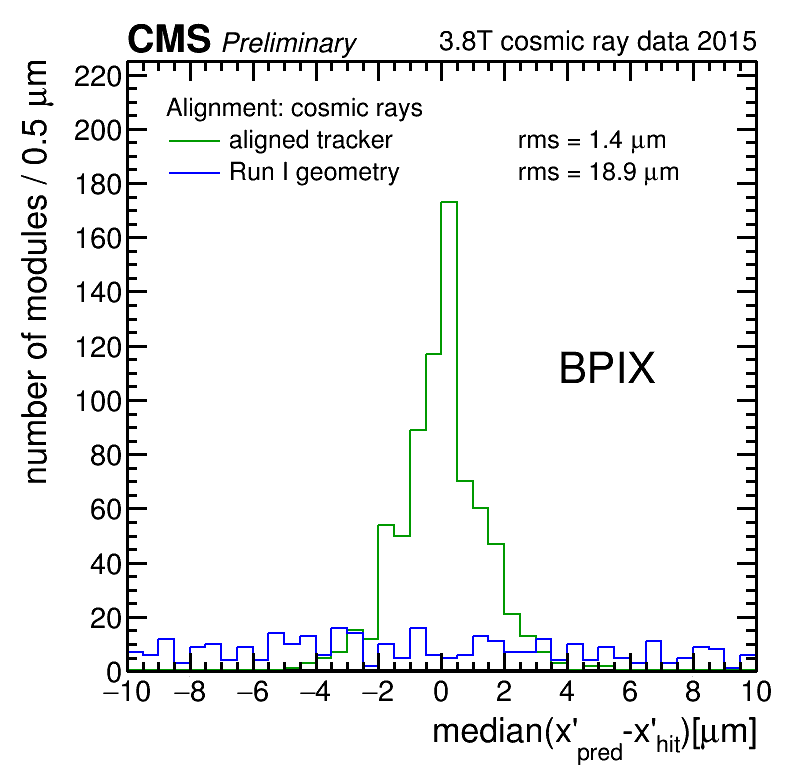
\includegraphics[width=0.45\textwidth]{../figs/Alignment/AlRes_CRAFT_DmedianR_BPIX_plain.png}\includegraphics[width=0.45\textwidth]{../figs/Alignment/AlRes_CRAFT_DmedianYR_BPIX_plain.png}
    \end{center}
    \caption {DMRs for the local $x$-direction (left) and for the local $y$-direction (right) in the BPIX of the CMS tracking system, using~2 million cosmic ray tracks collected with the magnetic field of $B=3.8$T. The blue line shows the Run~I geometry. The green line shows the alignment produced with the Millepede-II and HIP algorithms using cosmic ray data at $B=0$T and $B=3.8$T.}
    \label{fig:DMRs}
\end{figure}

\subsection{Cosmic Track Splitting Validation}
\label{sec:AlRes_trackSplit}

% (8) ALMOST QUOTE
%Cosmic ray tracks are split in half at the hit closest to origin and refitted with the alignment constants under consideration. The differences in various track parameters between the two half-tracks are studied. The width of the distribution measures the achieved alignment precision, while deviations from zero indicate possible biases. 
%Results of the cosmic track splitting validation are shown in Fig.~\ref{fig:trackSplit}. The normalized differences between two halves of a cosmic track, split at the point of closest approach to the interaction region, in $d_{xy}$ (Fig.~\ref{fig:trackSplit}, left), the $xy$ distance between the track and the origin, and in $d_z$ (right), the distance in the $z$ direction between the track and the origin. The observed precision using the aligned geometry (green circles), produced with the Millepede-II and HIP algorithms using cosmic ray data at $B=0$T and $B=3.8$T, is a major improvement over the Run~I geometry (blue empty squares). The precision comes close to that of the ideal Monte Carlo, illustrating that the tracker has almost reached its design spatial resolution.
% (8) MY WORDS:
To perform the cosmic track splitting validation, cosmic tracks are split into two parts at the hit closest to the center of the detector and both parts are reconstructed separately using alignment results. After that, the distributions of the differences in track parameters are prepared. The RMS values of the distributions are measures of the precision of the alignment constants. A deviation of a central value from zero would indicate a bias. The results of this validation for~2015 alignment are shown in Fig.~\ref{fig:trackSplit}.

\begin{figure}[htb]
    \begin{center}
        \includegraphics[width=0.45\textwidth]{../figs/Alignment/AlRes_CRAFT_hist_Delta_dxy.png}\includegraphics[width=0.45\textwidth]{../figs/Alignment/AlRes_CRAFT_hist_Delta_dz.png}
    \end{center}
    \caption{Results of the cosmic track splitting validation. The normalized differences between two parts of a cosmic track in the $xy$ distance between the track and the origin ($d_{xy}$, left), and in the distance in the $z$ direction between the track and the origin ($d_z$, right). Alignment is produced with the Millepede-II and HIP algorithms using cosmic ray data at the magnetic field of $B=0$T and~$B=3.8$T of CMS solenoid. Aligned geometry is shown in green.}
    \label{fig:trackSplit}
\end{figure}

\subsection{Primary Vertex Validation}
\label{sec:AlRes_PVvalid}

% (10) NO PLAGIARISM DETECTED
The resolution of the reconstructed vertex position is driven by the pixel subdetectors as the closest subdetectors to the interaction point which also have the best hit resolution. The primary vertex validation is based on the study the distances between tracks and the reconstructed vertex. 

%(11) NO PLAGIARISM DETECTED
Figure~\ref{fig:PVvalidation} compares the previous alignment to the one of a previous alignment reached during the commissioning phase with cosmic ray tracks at full magnetic field and to a detailed detector simulation with perfect alignment and calibration. The structures of the green curve indicate relative movements of the pixel half-barrels.

\begin{figure}[htb]
    \begin{center}
        \includegraphics[width=0.45\textwidth]{../figs/Alignment/AlRes_dxyPhiBiasCanvas.pdf}\includegraphics[width=0.45\textwidth]{../figs/Alignment/AlRes_dzPhiBiasCanvas.png}
    \end{center}
    \caption{The results of the primary vertex validation. The distance of the track at its closest approach to a refit unbiased primary vertex ($d_{xy}$, left and $d_z$, right) in the transverse plane. The validation is produced with $B=0$T collision data. The alignment is produced with the Millepede-II and HIP algorithms using ~$B=0$T and~$B=3.8$T cosmic ray data and $B=0$T collision data. }
    \label{fig:PVvalidation}
\end{figure}

%\begin{figure}[htb]
%    \begin{center}
%        \includegraphics[width=0.98\textwidth]{../figs/Alignment/global_tracker_2_final.png}
%    \end{center}
%    \caption{Geometry comparison plot of CRUZET 2015 object vs Run I.}
%    \label{fig:trackAndResiduals}
%\end{figure}

%(12) NO PLAGIARISM DETECTED
Given the complexity of the CMS detector, any single measurement based on CMS data requires an excellent understanding of the geometry and response of all systems to particles of all types. The CMS Alignment and Calibration team coordinates hundreds of CMS physicists who are working on various aspects of this. The Chapter~\ref{sec:alignment} of this dissertation presented one aspect of this work that concerns alignment of one system of CMS, the part in which the author of this dissertation played an important role.


\chapter{$W\gamma$ Cross Section Measurement}
\label{sec:AN_WgMeas}

The goal of this research is to measure the total and differential cross section of the $W\gamma$ production in $pp$ collisions as a function of the photon transverse momentum $P_T^\gamma$ at~$\sqrt{s}=8$~TeV center-of-mass collision energy. Decay channels $W\rightarrow\mu\nu$ and $W\rightarrow e\nu$ are considered. The measurement is performed using CMS data collected in~2012.

 % 30 pages
%% Explain analysis outline here
%\section{Data and Simulation Samples}

%\subsection{Object and Event Selection}

%\section{Background Estimation and Subtraction}

%\section{Detector Resolution Unfolding}

%\section{Acceptance and Efficiency}

%\subsection{Systematic Uncertainties}

%\section{Cross Section}


%\chapter{Summary and Conclusions}
\label{sec:Conclusions}

This dissertation reports a measurement of the total and differential cross sections, $\sigma$ and $\frac{d\sigma}{dP_T^{\gamma}}$, of the $W\gamma$ production in the muon and the electron channels using full~2012 dataset of $L=$19.6~fb$^{-1}$ collected by CMS at $\sqrt{s}=$8~TeV. This is the first measurement of the differential cross section of the $W\gamma$ production at the CMS experiment. The results are in agreement between two channels and also agree with the predictions computed at NLO using the MCFM program and the Madgraph~5 Monte Carlo generator. The agreement with theory means agreement with the MC predictions with no clear indication of new physics.

The differential cross section measurement has the special significance because a new physics would be difficult to detect in the total production cross section, however accurate measurement of the differential cross section with respect to an observable kinematic variable of the final state particles, and especially with respect to the $P_T^{\gamma}$, are sensitive probes to BSM models. The results of the differential spectrum measurement could be used to set limits on aTGC constants.

In addition to $W\gamma$ cross section, we also measure $Z\gamma$ cross section and compare results with the published $Z\gamma$ CMS measurement at $\sqrt{s}=$8~TeV. The good agreement between our and published results on $Z\gamma$ cross section validates parts of our $W\gamma$ measurement that are the same between $Z\gamma$ and $W\gamma$ measurements including lepton and photon selection, jets$\rightarrow\gamma$ background estimation, detector resolution unfolding, acceptance and efficiency corrections.

Measurements of $W\gamma$ and the other diboson and triboson productions at higher energies and luminosities will have more opportunities to discover a new physics if it is present. That is one of the reasons why these measurements remain a significant part of CMS physics program for studies at $\sqrt{s}=$13~TeV.

%  \begin{itemize}
%     \item Cross section for muon and electron channels are computed 
%     \item This is the first measurement of the differential $W\gamma$ cross section with CMS
%     \item Results agree with the MC prediction
%     \item Results between the two channels agree
%     \item Relative systematic uncertainties on total cross section are larger than those reported by the CMS 7 TeV measurement
%     \item Good agreement in the $Z\gamma$ check validates most parts of the analysis (those which are the same for the muon and electron channels)
%  \end{itemize}
 % 1-2 pages

\begin{thebibliography}{1}
% Intro
\bibitem{ref_Griffiths} Griffiths textbook
\bibitem{ref_fig_SM} website: http://www.isgtw.org/spotlight/go-particle-quest-first-cern-hackfest
\bibitem{ref_HiggsPaperCMS} CMS Paper about Higgs boson discovery
\bibitem{ref_HiggsPaperATLAS} ATLAS Paper about Higgs boson discovery
\bibitem{ref_fig_PDFs} website: https://mstwpdf.hepforge.org/
% WgAbout
\bibitem{ref_PDG} PDG
% LHC/CMS

% Alignment

% AN

\end{thebibliography}


% Appendices



\end{document}

